\documentclass[review]{elsarticle}

\usepackage{lineno,hyperref}
\usepackage{helvet}
\usepackage{courier}
\usepackage[T1]{fontenc}
\usepackage{ae,aecompl}
\usepackage{amsmath,amsfonts,amsthm,amssymb}
\usepackage{url}
\usepackage[usenames]{color}

\usepackage{bbm}
\usepackage[usenames]{color}
\usepackage{wrapfig}
\usepackage{booktabs}
\usepackage[usenames,dvipsnames]{xcolor}
\usepackage[ruled,vlined,linesnumbered]{algorithm2e}
\usepackage{graphicx}
\usepackage{xspace}
\xspaceaddexceptions{]\})(}
\usepackage[usenames]{color}
\usepackage{comment}


\newtheorem{definition}{Definition}
\newtheorem{theorem}{Theorem}
\newtheorem{corollary}{Corollary}
\newtheorem{lemma}{Lemma}
\newtheorem{example}{Example}


\newcommand{\argmin}{\operatornamewithlimits{argmin}}
\newcommand{\argmax}{\operatornamewithlimits{argmax}}

\newcommand{\tuple}[1]{\ensuremath{\left \langle #1 \right \rangle }}
\newcommand{\mddr}{\ensuremath{MDD_R}\xspace}
\newcommand{\mddrs}{\ensuremath{MDD_R}s\xspace}
\newcommand{\implicitct}{\textit{ImplicitCT}\xspace}
\usepackage{amsmath}
\usepackage{amsthm}
\usepackage{amssymb}
\usepackage{color, colortbl}
\definecolor{LightCyan}{rgb}{0.88,1,1}


\usepackage[usenames,dvipsnames]{xcolor}
\usepackage[ruled,vlined,linesnumbered]{algorithm2e}

\usepackage{pifont}% http://ctan.org/pkg/pifont
\newcommand{\cmark}{\ding{51}}%
\newcommand{\xmark}{\ding{55}}%

\usepackage{rotating}
\usepackage{multirow}
\usepackage{subfigure}
%\usepackage{subcaption} \roni{This causes a compilation error}

\newcommand{\commentout}[1]{ }

\newcommand{\history}{past-conflicts\xspace}

\newcommand{\target}{\ensuremath{G}\xspace}
\newcommand{\cost}{\textit{cost}}
\newcommand{\source}{\ensuremath{S}\xspace}
\newcommand{\graph}{\ensuremath{\mathcal{G}}\xspace}
\newcommand{\fromv}{\ensuremath{\mathit{from}}\xspace}
\newcommand{\tov}{\ensuremath{\mathit{to}}\xspace}
\newcommand{\decidet}{\ensuremath{\mathit{DECIDE_T}}\xspace}
\newcommand{\decidemapfr}{\ensuremath{\mathit{DECIDE_{MAPF_R}}}\xspace}
\newcommand{\decidemapf}{\ensuremath{\mathit{DECIDE_{MAPF}}}\xspace}



%
% Add comments in the text
%
\newboolean{showcomments}
\setboolean{showcomments}{true}
%\setboolean{showcomments}{false}

\ifthenelse{\boolean{showcomments}}
  {\newcommand{\nb}[3]{
  {\color{#2}\small\fbox{\bfseries\sffamily\scriptsize#1}}
  {\color{#2}\sffamily\small$\triangleright~$\textit{\small #3}$~\triangleleft$}
  }
  }
  {\newcommand{\nb}[3]{}
  }

\newcommand\konstantin[1]{\nb{\textbf{Konstantin:}}{red}{#1}}
\newcommand\anton[1]{\nb{\textbf{Anton:}}{cyan}{#1}}
\newcommand\roni[1]{\nb{\textbf{Roni:}}{green}{#1}}
\newcommand\pavel[1]{\nb{\textbf{Pavel:}}{blue}{#1}}
\newcommand\dor[1]{\nb{\textbf{Dor:}}{Fuchsia}{#1}}


% \theoremstyle{definition}
% \newtheorem{example}{Example}[section]

%\usepackage[smaller]{acronym}
\usepackage{acronym}
\acrodef{SOC}{sum of costs}
\acrodef{SIPP}{Safe Interval Path Planning}
\acrodef{CSIPP}{Constrained Safe Interval Path Planning}
\acrodef{CBS}{Conflict-Based Search}
\acrodef{CCBS}{Continuous-time Conflict-Based Search}
\acrodef{MAPF}{Multi-Agent Pathfinding}
\acrodef{ICTS}{Increasing Cost Tree Search}
\acrodef{MCCBS}{Multi-Constraint CBS}
\acrodef{CT}{Constraint Tree}
\acrodef{SMT}{SAT Modulo Theory}
\acrodef{PS}{Propositional Skeleton}

\newcommand{\smt}{\ac{SMT}\xspace}
\newcommand{\ccbs}{\ac{CCBS}\xspace}
\newcommand{\cbs}{\ac{CBS}\xspace}
\newcommand{\ct}{\ac{CT}\xspace}
\newcommand{\sipp}{\ac{SIPP}\xspace}
\newcommand{\csipp}{\ac{CSIPP}\xspace}
\newcommand{\ps}{\ac{PS}\xspace}



\newcommand{\astar}{A$^*$\xspace}

\newcommand{\mapfr}{\ac{MAPF}$_R$\xspace}

\newcommand{\mddsat}{MDD-SAT\xspace}

\newcommand{\smtcbsO}{SMT-CBS\xspace} % O like original smt-cbs
%\newcommand{\smtcbs}{SMT-CCBS\xspace} % both smtcbs and smtccbs are the same; for the original smt-cbs use smtcbsO
\newcommand{\smtccbs}{SMT-CCBS\xspace}
\newcommand{\musmtccbs}{\ensuremath{\mu}SMT-CCBS\xspace}


\newcommand{\mapfect}{\mapfr-CT\xspace}

\newcommand{\mapf}{\ac{MAPF}\xspace}
\newcommand{\const}{\textit{const}\xspace}
\newcommand{\safe}{\textit{Safe}\xspace}
\newcommand{\true}{\textit{true}\xspace}
\newcommand{\false}{\textit{false}\xspace}
\newcommand{\timep}{\textit{time}\xspace}

\newcommand{\coord}{\textit{coord}\xspace}
\newcommand{\iscollision}{\textsc{IsCollision}\xspace}
\newcommand{\inconflict}{\textsc{InConflict}\xspace}
\newcommand{\OPEN}{\textsc{Open}\xspace}



\newcommand{\shortcite}{\cite}

\modulolinenumbers[5]

\journal{Artificial Intelligence Journal}

%%%%%%%%%%%%%%%%%%%%%%%
%% Elsevier bibliography styles
%%%%%%%%%%%%%%%%%%%%%%%
%% To change the style, put a % in front of the second line of the current style and
%% remove the % from the second line of the style you would like to use.
%%%%%%%%%%%%%%%%%%%%%%%

%% Numbered
%\bibliographystyle{model1-num-names}

%% Numbered without titles
%\bibliographystyle{model1a-num-names}

%% Harvard
%\bibliographystyle{model2-names.bst}\biboptions{authoryear}

%% Vancouver numbered
%\usepackage{numcompress}\bibliographystyle{model3-num-names}

%% Vancouver name/year
%\usepackage{numcompress}\bibliographystyle{model4-names}\biboptions{authoryear}

%% APA style
%\bibliographystyle{model5-names}\biboptions{authoryear}

%% AMA style
%\usepackage{numcompress}\bibliographystyle{model6-num-names}

%% `Elsevier LaTeX' style
\bibliographystyle{elsarticle-num}
%%%%%%%%%%%%%%%%%%%%%%%

\begin{document}

\begin{frontmatter}

%\title{Conflict-Based Search with Continuous Time and Space}
%\title{Multi-Agent Pathfinding with Continuous Time and Euclidean Space (maybe remove the last 3 words?)}
\title{Multi-Agent Pathfinding with Continuous Time}
%\title{Multi-Agent Pathfinding with Continuous Time}

%\tnotetext[mytitlenote]{Fully documented templates are available in the elsarticle package on \href{http://www.ctan.org/tex-archive/macros/latex/contrib/elsarticle}{CTAN}.}





%% Group authors per affiliation:

%% Group authors per affiliation:
%\author{Elsevier\fnref{myfootnote}}
%\address{Radarweg 29, Amsterdam}
%\fntext[myfootnote]{Since 1880.}

%% or include affiliations in footnotes:
\author[ras,rudn]{Anton Andreychuk}
\author[ras,hse,mipt]{Konstantin Yakovlev\corref{mycorrespondingauthor}}
%\ead{support@elsevier.com}
\author[cvut]{Pavel Surynek}
\author[bgu]{Dor Atzmon}
\author[bgu,parc]{Roni Stern}

\address[ras]{Federal Research Center for Computer Science and Control of Russian Academy of Sciences, Russia}
\address[hse]{National Research University Higher School of Economics, Russia}
\address[mipt]{Moscow Institute of Physics and Technology, Russia}
\address[rudn]{Peoples' Friendship University of Russia (RUDN University), Russia}
\address[bgu]{Software and Information Systems Eng., 
Ben Gurion University of the Negev, Israel}
\address[parc]{System Sciences Laboratory (SSL), Palo Alto Research Center (PARC), USA}
\address[cvut]{Faculty of Information Technology (FIT), Czech Technical University (\v{C}VUT), Czech Republic}



%\author{Konstantin Yakovlev, Anton Andreychuk, Pavel Surynek, Dor Atzom, and Roni Stern}
%\address{The Department of Software and Information Systems Engineering\\ Ben Gurion University of the Negev}

%\author{Elsevier\fnref{myfootnote}}
%\address{Radarweg 29, Amsterdam}
%\fntext[myfootnote]{Since 1880.}

%% or include affiliations in footnotes:
%\author[mymainaddress,mysecondaryaddress]{Elsevier Inc}
%\ead[url]{www.elsevier.com}

%\author[mysecondaryaddress]{Global Customer Service\corref{mycorrespondingauthor}}
%\cortext[mycorrespondingauthor]{Corresponding author}
%\ead{support@elsevier.com}

%\address[mymainaddress]{1600 John F Kennedy Boulevard, Philadelphia}
%\address[mysecondaryaddress]{360 Park Avenue South, New York}


\begin{abstract}

\mapf is the problem of finding paths for multiple agents such that each agent reaches its goal and the agents do not collide. 
In recent years, variants of \mapf have risen in a wide range of real-world applications such as warehouse management and autonomous vehicles.
Optimizing common \mapf objectives, such as minimizing sum-of-costs or makespan is computationally intractable, but state-of-the-art algorithms are able to solve optimally problems with dozens of agents.
However, most \mapf algorithms assume that 
(1) time is discretized into time steps and
(2) the duration of every action is one time step. 
%,  and (3) in every time step each agent occupies exactly a single location.
These simplifying assumptions limit the applicability of \mapf algorithms in real-world application and raise non-trivial questions such as how to discretize time in an effective manner. 
We propose two novel \mapf algorithms, \ccbs and \smtccbs, that do not discretize time and allow arbitrary action duration. 
\ccbs draws on ideas from \sipp, a single-agent pathfinding algorithm designed to cope with dynamic obstacles, and \cbs, a state-of-the-art search-based \mapf algorithm. 
\smtccbs builds on similar ideas, but is based on a different state-of-the-art \mapf algorithm called \smtcbsO, which applied a SAT Modulu Theory (SMT) problem-solving procedure. 
\ccbs guarantees to return solutions that have  minimal sum-of-costs, while \smtccbs guarantees to return solutions that have minimal makespan. 
We implemented \ccbs and \smtccbs and evaluated them on grid-based \mapf problems and general graphs (roadmaps). 
The results show that both algorithms can efficiently solve optimally non-trivial \mapf problems.
\end{abstract}

\begin{keyword}
%\texttt{elsarticle.cls}\sep \LaTeX\sep Elsevier \sep template
Multi-Agent Pathfinding\sep Conflict-Based Search\sep Safe-Interval Path Planning\sep SAT modulo Theory\sep Heuristic Search
%\MSC[2010] 00-01\sep  99-00
\pavel{Why not to add abbreviations Conflict-Based Search (CBS), (SIPP), (SMT), MAPF, \mapfr, ...(add not replace)}
\roni{I think it makes more sense to leave it as is, and not use the abbreviation.}
\end{keyword}

\end{frontmatter}

\linenumbers



\section{Introduction}
%TODO: Roni

% COPY AND PASTE FROM WORKSHOP PAPER

% What is MAPF
\mapf is the problem of finding paths for multiple agents such that each agent reaches its goal and the agents do not collide. \mapf has topical applications in warehouse management~\cite{wurman2008coordinating}, airport towing~\cite{morris2016planning}, autonomous vehicles, robotics~\cite{veloso2015cobots}, and digital entertainment~\cite{ma2017feasibility}.
%Finding a solution to some \mapf problems can be done in polynomial time~\cite{kornhauser1984coordinating}\roni{See the reference I added. This is a new result by Bernhard Nebel. He proved that MAPF for directed graphs is NP Hard. To be honest, I did not read his proof yet, but I know he did it. It is a funny story: in the ICAPS MAPF tutorial Roman et al. and I gave, he asked if we the Kornhauser results holds for directed graphs. I told him I think it does but I'm not sure. So, half a year later, he proved me wrong :)} while for others it is NP hard~\cite{nebel2020computational}. \konstantin{I'm not sure that this phrase is correct as finding a solution for \emph{any} MAPF problem is polynomial as long as we do not care about the optimality of the solution.} 
% MAPF is hard
A common requirement in \mapf applications is to minimize either the \emph{sum-of-costs} (SOC) of the agents' plans 
or their maximum, which is also known as \emph{makespan}. %\konstantin{may be we need to briefly say here what is the makespan? Or it is considered to be evident to any reader?}\roni{Added text to fix this.} 
Finding \mapf solutions that have minimal SOC or minimal makespan are both NP hard problems~\cite{surynek2010optimization,yu2013structure}.  
Nevertheless, AI researchers in the past years have made substantial progress in finding solutions with minimal SOC or minimal makespan for a growing number of \mapf problems, including problems with over one hundred agents~\cite{sharon2015conflict,sharon2013increasing,wagner2015subdimensional,standley2010finding,felner2018adding,ICTAIpicat,yu2013structure}. 


%\konstantin{The planner that we propose can not handle hundreds of agents optimally. May be we should re-phrase this sentence?}\roni{I think it is Ok. We are solving a harder problem, so OK if we solve smaller problems.}


% Prior work assumptions: unit-cost, discrete time, agents without any shape
However, most prior work assumed that 
(1) time is discretized into time steps and
(2) the duration of every action is one time step. 
These simplifying assumptions limit the applicability of \mapf algorithm in real-world applications. Discretizing time raises the challenge of how to choose the granularity of the discretization. Assuming the duration of all actions is identical ignores kinematics and variable speeds. 
Therefore, in this work we do not make any of these simplifying assumptions and address a more general \mapf problem in which time is not discretized, actions can have arbitrary duration, and agents occupy an defined area in a metric space. This problem is called \mapfr~\cite{walker2018extended}.\footnote{We discuss later the relation between Walker et al.'s~\cite{walker2018extended} definition of \mapfr and ours.}


% Our contribution: 
We propose two novel \mapf algorithms for solving \mapfr. 
The first algorithm is called \ccbs. \ccbs builds on two existing algorithms: 
\sipp~\cite{phillips2011sipp} and \cbs~\cite{sharon2015conflict}. 
\sipp is a  single-agent pathfinding algorithm designed to find paths that avoid dynamic obstacles. %\konstantin{SIPP is not about continuous time initially}. \roni{Fixed}
\cbs is a state-of-the-art search-based \mapf algorithm with many extensions and improvements. 
\ccbs follows the same problem-solving framework as \cbs, but uses a novel \sipp to plan paths for the individual agents, and imposes a novel type of constraints to resolve conflicts between the resulting plans. We prove that \ccbs is sound, complete, and returns solutions that have minimal SOC. 
The second algorithm we propose is called \smtccbs. 
\smtccbs resolves conflicts between agents using the same type of constraints as \ccbs. 
However, it does so in the \smt problem solving framework used by the \smtcbsO algorithm~\cite{DBLP:conf/ijcai/Surynek19} to solve \mapf problems. 
%he \mapfr \smtccbs in a way similar to how \ccbs 
%\smtccbs builds on \smtcbsO \cite{DBLP:conf/ijcai/Surynek19}, which is a  state-of-the-art algorithm that applies an \smt problem solving procedure to \mapf. In \smtcbsO, a sequence of Boolean satisfiability (SAT) problems
%compiles \mapf to a sequence of Boolean satisfiability (SAT) problems and solves them with an off-the-shelf SAT solver. 
%\smtccbs works in a similar way, but compiles \mapfr to a sequence of \smt problems, where the underlying \emph{theory} is the movement rules in \mapfr. %We then propese an \smt solver in which a variant of \sipp is used to implement this theory is then applied to solve the formula. [roni: not sufficiently clear]
\smtccbs is sound, complete, and returns solution that have minimal makespan. 
%\roni{Edited the above, please check}\konstantin{I see no problems with the above text. It's good.}GReat!


% Experimental results
We implemented \ccbs and \smtccbs, and evaluated them on standard grid-based \mapf benchmarks as well as generated roadmaps. 
The results show that both algorithms can solve \mapf problems with dozens of agents optimally. 
While we are not not the first to study \mapf beyond its basic setting~\cite{walker2018extended,li2019multi,cohen2019optimal}, to the best of our knowledge we are the first to propose \mapf algorithms that can handle agents with volumes and non-uniform action durations while avoiding any form of time discretization (see Section~\ref{sec:related-work} for a more detailed discussion).  
%\konstantin{may be we better put the cross-reference to the Related Work section here?}Roni: fixed
%~\cite{walker2018extended,li2019multi}.  However, to the best of our knowledge, the algorithms we propose are the first \mapf algorithms that can handle arbitrary directly consider handle non-discretized, i.e. continuous, time, non-grid domains, non-unit actions duration, agents with a volume, and are still optimal and complete. A more detailed discussion is given later in Section~\ref{sec:related-work}. 
All our implementations are publicly available, so future researchers can reproduce our results and build on them. 

%The results also show that using our algorithms enables one to find solutions that cost less than solutions generated by \mapf algorithms that discretize time. \konstantin{Right now we do not have a section in the paper desribinf the latter effect. Although it would be nice to have it as agreed before.} \roni{TODO: Add it}\roni{well, we do have advantage over k=2, but not much. I'll just comment it out.}
%\roni{TODO: Verify ? signs in completeness column}Done!
%Since \ac{CCBS} considers agents' geometric shape and  continuous time, the cost of collision detection in \ac{CCBS} is significantly higher than in \cbs. To mitigate this, we propose a history-based heuristic, that attempts to avoid some collision detection checks by guessing which pair of agents are likely to have a conflict. We discuss the relation between this heuristic and the concept of cardinal conflicts~\cite{boyarski2015icbs}, and propose a simple hybrid heuristic that combines these methods and works well.  
% A bit of related work

%We are not the first to study \mapf beyond its basic setting.  Some addressed agents with %~\cite{walker2018extended,li2019multi}.  However, to the best of our knowledge, the algorithms we propose are the first \mapf algorithms that can handle arbitrary directly consider handle non-discretized, i.e. continuous, time, non-grid domains, non-unit actions duration, agents with a volume, and are still optimal and complete. A more detailed discussion is given later in Section~\ref{sec:related-work}. 
%\konstantin{When I started reading the paper 'from the clean slate' I got puzzled a bit with that table right here. IT seemed a bit out-of-the context to me. Maybe we just skip this phrase?}


A preliminary version of this work was published in two conferences~\cite{andreychuk2019multi,DBLP:conf/socs/Surynek19}.  
%\roni{Pavel, can you add a reference to your preliminary work? } \pavel{Added, bud I suggest: "A preliminary version of CCBS algorithm was published in ... and SMT ...}
The main contribution of this journal paper is to present these works in a unified and coherent manner. In addition, this journal paper extends these works significantly, by providing:
\begin{itemize}
    \item A formal proof of completeness and optimality for \ccbs and \smtccbs.
    %\roni{Ideally we will also have this for \smtccbs . But, I wouldn't delay submission}
    %\konstantin{I agree that ideally we should have this fo \smtccbs as well.}
    \item A detailed explanation of the algorithms and include a running example to illustrate their behavior. 
    \item A detailed description of how one can implement collision and conflict detection, and unsafe interval calculation.
    \item A comprehensive set of experiments, including experiments on roadmaps. 
\end{itemize}

%\roni{Maybe we have more? not critical} \konstantin{May be should say smth. about that in this work we explicitly elaborate on how auxiliary functions like \inconflict might be implemented withtin the suggested framework (this was only briefly mentioned before in the conference papers).}\roni{Done. Maybe we can say more. Not important though.}

This paper is structured as follows. 
Section~\ref{sec:background} provides relevant \mapf definitions and relevant background. 
Section~\ref{sec:problem-statement} formally defines the \mapfr problem we address. 
Section~\ref{sec:ccbs} presents the \ccbs algorithm and Section~\ref{sec:smtccbs} presents \smtccbs. Results of the empirical evaluation of both algorithms are described in Section~\ref{sec:experiments}. 
A detailed discussion of related work is given in Section~\ref{sec:related-work}, 
and Section~\ref{sec:conclusion} concludes with a list of directions for future work. 


\section{Background}
\label{sec:background}

%Classical MAPF
A \emph{classical MAPF} problem~\cite{stern2019mapf} with $k$ agents is defined by 
a tuple $\langle \mathcal{G}, \source,\target \rangle$ 
where $\mathcal{G}=(V,E)$ is an undirected graph, 
$\source:[1,\ldots,k]\rightarrow V$ maps an agent to a start vertex, 
and $\target:[1,\ldots,k]\rightarrow V$ maps an agent to a goal vertex (see Fig.~\ref{fig:classical-mapf}.

% Time and actions
Time is discretized into time steps. 
For every time step $t$, each agent occupies one of the graph vertices, referred to as the \emph{location} of that agent at time $t$.
%\dor{$t$ represents both target vertex and time.} \konstantin{I suggest 'g' for the goal vertices} 
An \emph{action} in classical MAPF is a function $a: V\rightarrow V$ 
such that $a(v)=v'$ means the agent's current location is $v$ and its location in the next time step is $v'$. %\dor{Maybe we should formally mention that there is an edge between v and v'.}
In every time step each agent can choose to perform an action. 
There are two types of actions: a \emph{wait} action, in which the agent stays in its location, and a \emph{move} action, in which the agent moves to one of the vertices adjacent to its current location. 


%\konstantin{I don't like that actions do not have a time dimension as part of the definition, although I understand that for classical MAPF this is not 100\% needed}
%\roni{Good point. but this is how it is usually defined. When we get to our problem def we will add the time aspect.}


% A solution to a MAPF problem
A sequence of actions $\pi_i=(a_1,\ldots,a_n)$ 
is a \emph{single-agent plan} for agent $i$ 
if $a_n(a_{n-1}(\cdots(a_1(\source(i)))\cdots))=\target(i)$, i.e., if it leads the agent from its start to its goal. A \textbf{solution} to a classical MAPF problem is a set of $k$ single-agent plans, one for each agent.  

%We denote by $\pi_r[x]$ the location of agent $r$ after executing the first $x$ actions in $\pi$, starting from the agent's source $s(r)$. 
%\konstantin{Do we actually need $\pi_i[x]$? I also don't like that the agent is a parameter, i.e. $s(i)$, maybe we use superscripts instead like $s^i$ or $s^(i)$}\roni{I understand, both options are Ok. I'm keeping it as is, for now, but in the end, your the lead and I can change to your preference.} 


\begin{figure}
    \centering
    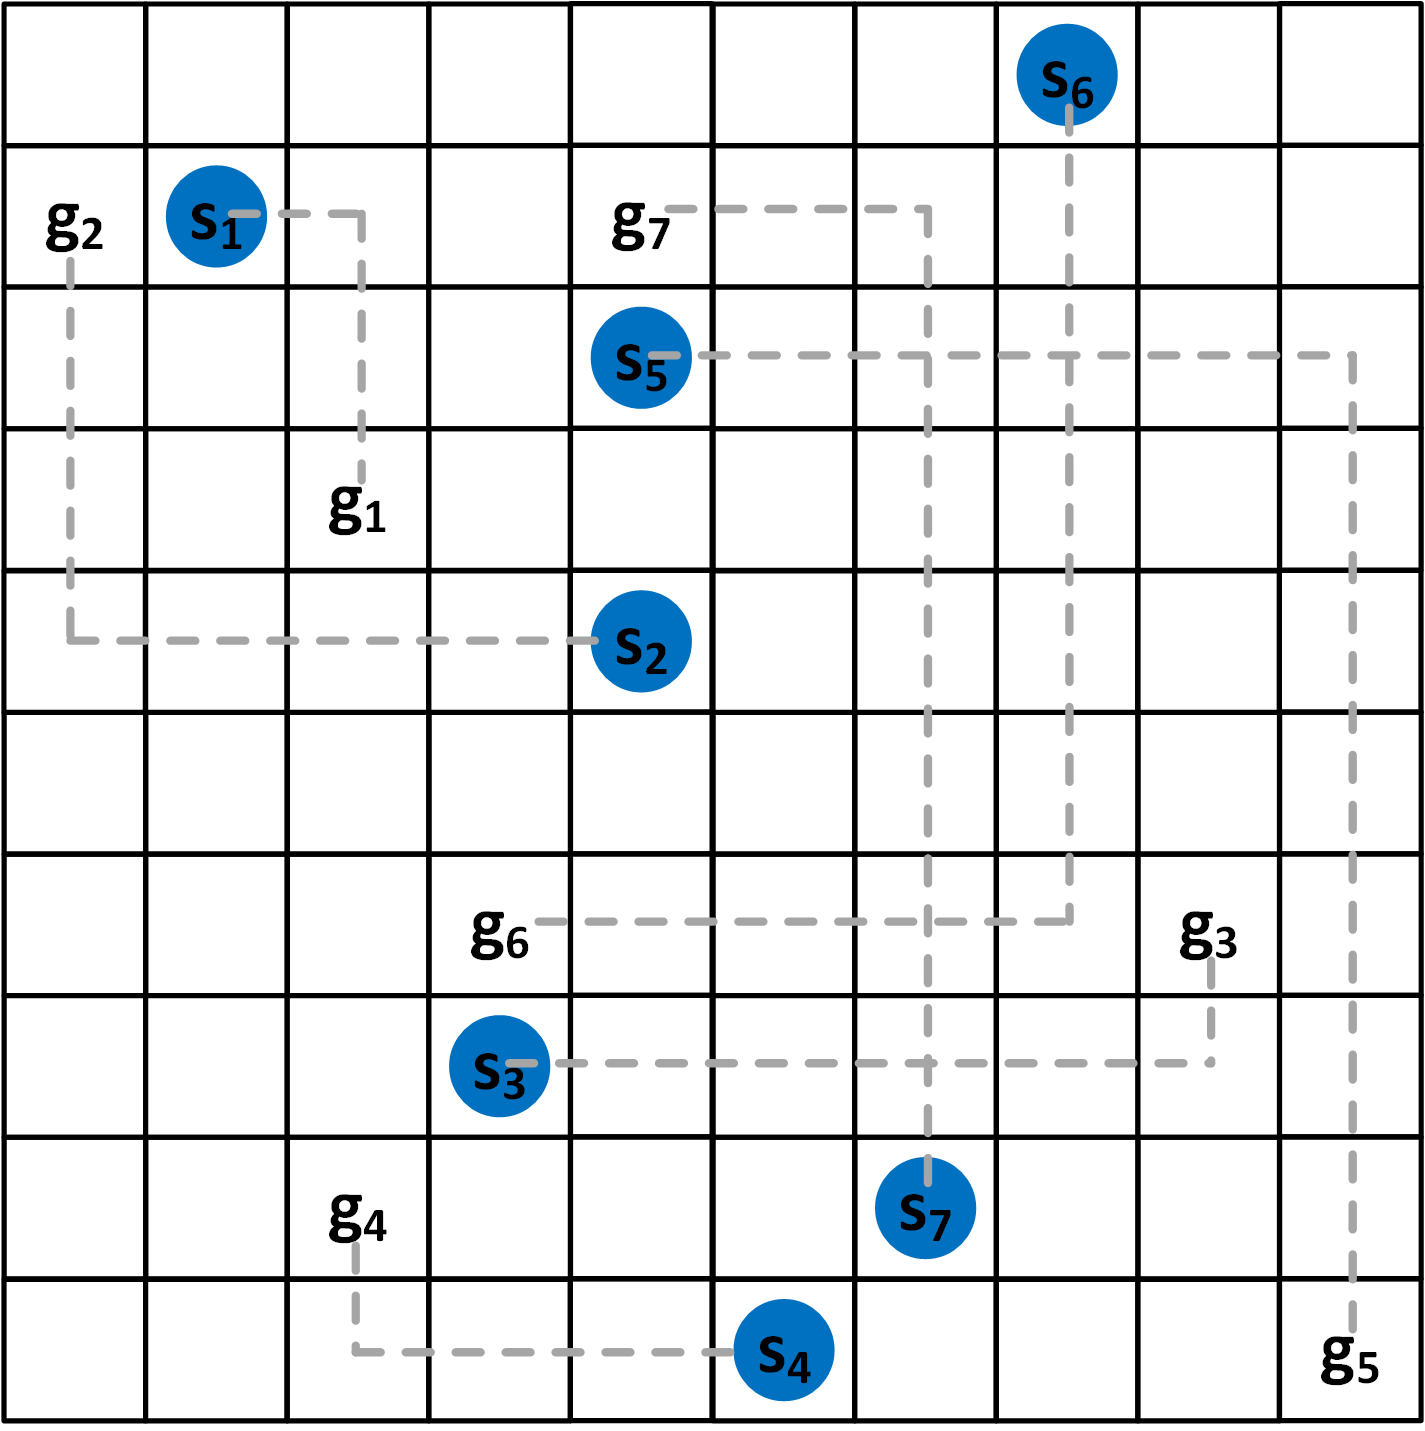
\includegraphics[width=0.5\linewidth]{classical-mapf-grid-example.png}
    \caption{An example of a classical MAPF problem instance on a 4-connected grid.}
    \label{fig:classical-mapf}
\end{figure}

\begin{figure}
    \centering
    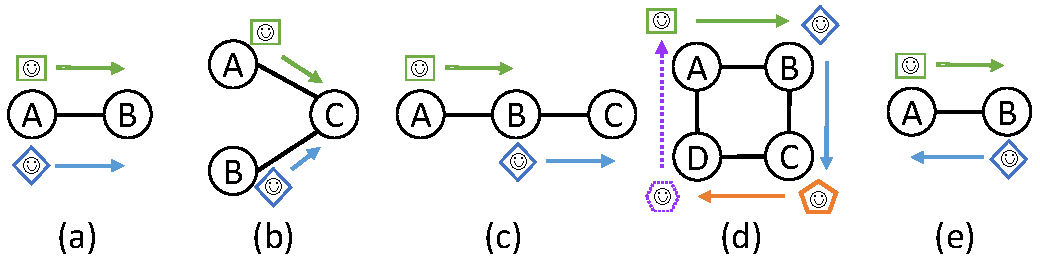
\includegraphics[width=\columnwidth]{types-of-conflicts.pdf}
    \caption{An illustration from~\cite{stern2019mapf} of an edge conflict (a), a vertex conflict (b), a following conflict (c), a cycle conflict (d), and a swapping conflict (e).}
    \label{fig:types-of-conflicts}
\end{figure}

% Conflicts and a valid solution in classical MAPF
A solution to a classical MAPF problem is \emph{valid} if its constituent single-agent plans do not \emph{conflict}. 
There are multiple types of conflicts. 
A \emph{vertex conflict} between single-plan $\pi_i$ for agent $i$ 
and single-plan $\pi_j$ for agent $j$ occurs at location $v$ and time step $t$ iff according to these plans agents $i$ and $j$ plan to occupy $v$ at the same time step $t$. We represent such a conflict by the tuple $\tuple{i,j,v,t}$. 
A \emph{swapping conflict} between single agent plans $\pi_i$ and $\pi_j$ occurs on edge $e$ at time step $t$ iff according to $\pi_i$ and $\pi_j$ both agents plan to traverse the edge $e\in E$ from opposite directions at the same time step $t$. We represent such a conflict by the tuple $\tuple{i,j,e,t}$. 
% An edge conflict between two single-agent plans occurs when the two corresponding agents are planned to perform the same action at the same location at the same time step.  A vertex conflict occurs when two agents are planned to occupy the same location at the same time. A swapping conflict occurs when two agents are planned to swap locations at the same time step. 
Figure~\ref{fig:types-of-conflicts} illustrates these conflicts as well as other types of conflict that arise in classical MAPF. See Stern et al.~\cite{stern2019mapf} for a deeper and more formal discussion of these conflicts. 

%\dor{Why are vertex and swapping conflicts defined between agents and an edge conflict between plans?}\roni{Only edge conflicts are w.r.t plans, and in its text we ``move'' to talking about who is planned to do what. I belive this is clear and easier to read}

% Action cost and objective functions in classical MAPF
In classical MAPF, every action incurs unit cost, 
and the cost of a single-agent plan is the number of its constituent actions. 
\emph{Sum-of-costs} (SOC) and \emph{makespan} are two common ways to define the cost of a set of single-agent plans $\Pi=(\pi_1,\ldots, \pi_k)$. The former is the summation over the costs of the constituent single-agent plans and the latter is their max. A solution to a \mapf problem is called SOC-optimal if it is valid and there is no valid solution that has a smaller SOC. A makespan-optimal solution is defined in a similar way. 
In general, the problem of finding SOC-optimal or makespan-optiaml solutions for a given \mapf problem is known to be NP hard~\cite{yu2013multi,surynek2010optimization}.

%, i.e., the plan's length.
%\konstantin{This definition doesn't look nice to me as 'length' may be understood in different ways. May be we come up with another definition?}\roni{Added to elaborate and better explain.}
%Some \mapf algorithms are guaranteed to return a solution with minimal SOC, while others guarantee makespan optimality. \konstantin{I would substitute the last phrase to 'In general solving classical MAPF optimally under either of those objectives is known to be NP-Hard (Yu and LaValle 2016)'.} \roni{Done}

%\roni{Maybe have here also some background on algorithms?}
%\konstantin{May be we add a section here with the overview of the prior work that deals with classical MAPF?}
%\roni{We have that below}

\subsection{Optimal Algorithms for Classical \mapf}
Several approaches have been proposed to find either SOC-optimal or makespan-optimal solutions for classical \mapf~ 
(e.g., see survey by Felner et al.~\cite{felner2017searchBased}). 
In this work, we build on three specific state-of-the-art classical \mapf solvers: \cbs~\cite{sharon2015conflict},   \mddsat~\cite{DBLP:conf/ecai/SurynekFSB16}, and \smtcbsO~\cite{DBLP:conf/ijcai/Surynek19}. 
For completeness, we provide a brief description of these algorithms here. 

\subsubsection{Conflict Based Search (CBS) for 
Finding SOC-Optimal Solutions}
\label{sec:cbs}

\cbs~\cite{sharon2015conflict} is a complete algorithm for classical \mapf that is guaranteed to return a SOC-optimal solution. 
It solves a given \mapf problem by finding a plan for each agent separately, detecting conflicts between these plans, and resolving them by replanning for the individual agents subject to specific \emph{constraints}. 

The basic \cbs implementation considers two types of conflicts: vertex conflicts and swapping conflicts. 
%A vertex conflict between plans $\pi_i$ and $\pi_j$ is defined by a tuple $\tuple{i,j,v,t}$, indicating that according to these plans agents $i$ and $j$ plan to occupy $v$ at the same time step $t$. A swapping conflict can be defined similarly by a tuple $\tuple{i,j,e,t}$, indicating that according to $\pi_i$ and $\pi_j$ both agents plan to traverse the edge $e\in E$ at the same time step, from opposite directions. 
%\dor{Is it an edge conflict or a swapping conflict?}\roni{Good catch}
Correspondingly, the basic \cbs implementation considers two types of constraints. 
A \cbs vertex-constraint is defined by a tuple $\tuple{i,v,t}$ and means that agent $i$ is prohibited from occupying vertex $v$ at $t$.  
A \cbs edge-constraint is defined similarly by a tuple $\tuple{i,e,t}$, where $e\in E$. To guarantee completeness and optimality, \cbs runs two search algorithms: a low-level search algorithm that finds plans for individual agents subject to a given set of constraints, and a high-level search algorithm that chooses which constraints to add. 
%\dor{I think that if we use "vertex-constraint", we should also use "vertex-conflict" (with hyphens).}
%\roni{It depends on context. It is different from how hyphens are used in Hebrew. We can talk about this. Also note it is a swapping conflict but we resolve it by adding an edge constraint.}


%completeness and optimality, \cbs runs two search algorithms: a low-level search algorithm that finds plans for individual agents subject to a given set of constraints, and a high-level search algorithm that chooses which constraints to add. \dor{I think that if we use "vertex-constraint", we should also use "vertex-conflict" (with hyphens).}

%The basic \cbs implementation considers two types of conflicts: a vertex conflict and an edge conflict. A vertex conflict between plans $\pi_i$ and $\pi_j$ is defined by a tuple $\tuple{i,j,v,t}$ and means that according to these plans agents $i$ and $j$ plan to occupy $v$ at the same time $t$. An edge conflict is defined similarly by a tuple $\tuple{i,j,e,t}$, and means that according to $\pi_i$ and $\pi_j$ both agents plan to traverse the edge $e\in E$ at the same time, from opposite directions. \dor{Is it an edge conflict or a swapping conflict?}


% CBS constraints
%A \cbs vertex-constraint is defined by a tuple $\tuple{i,v,t}$ and means that agent $i$ is prohibited from occupying vertex $v$ at $t$.  A \cbs edge-constraint is defined similarly by a tuple $\tuple{i,e,t}$, where $e\in E$. To guarantee completeness and optimality, \cbs runs two search algorithms: a low-level search algorithm that finds plans for individual agents subject to a given set of constraints, and a high-level search algorithm that chooses which constraints to add. \dor{I think that if we use "vertex-constraint", we should also use "vertex-conflict" (with hyphens).}

\paragraph{\textbf{\cbs: Low-Level Search}}
The task of the low-level search in \cbs is to find an optimal plan for an agent 
that is consistent with a given set of \cbs constraints. 
Any single-agent pathfinding algorithm that can do this can be used as the \cbs low-level search. 
To adapt single-agent pathfinding algorithms, such as \astar{}, to consider \cbs constraints, 
the search space must also consider the time dimension since a \cbs constraint $\tuple{i,v,t}$ 
blocks location $v$ only at a specific time step $t$. 
This means that a state in this single-agent search space is a pair $(v,t)$, representing that the agent is in location $v$ at time step $t$. Expanding such a state generates states 
of the form $(v',t+1)$, where $v'$ is either equal to $v$, representing a wait action, 
or equal to one of the locations adjacent to $v$. States generated by actions that violate the given set of \cbs constraints, are pruned. Running \astar{} on this search space returns the lowest-cost plan to the agent's goal that is consistent with the given set of \cbs constraints, as required. This adaptation of textbook \astar{} is very simple, and indeed most papers on \cbs do not report it and just mention that the low-level search of \cbs is \astar{}. 
%\footnote{\textbf{K: Again "A*" is missing. May be we also should say here that enhanced version of A* are also widely used, i.e. the ones that avoid expanding surplus nodes etc. Or I'm not right here?}}. \roni{I'm not sure thus some else did something more fancy than astar}

\paragraph{\textbf{\cbs: High-Level Search}}
The high-level search algorithm in \cbs works on a \ct, which is a binary tree, in which each node
$N$ is defined by a pair $(N.\const, N.\Pi)$ where 
$N.\const$ represents a set of \cbs constraints imposed on the agents and $N.\Pi$ is a \mapf solution that satisfies these \cbs constraints. A \ct node $N$ is generated by first setting its constraints ($N.\const$) and then 
computing $N.\Pi$ by running the low-level solver, which finds a plan for each agent subject to the constraints relevant to it in $N.\const$. If $N.\Pi$ does not contain any conflict, then $N.\Pi$ is a valid \mapf solution and $N$ is regarded as a goal node. Else, one of the conflicts $\tuple{i,j,x,t}$ (where $x$ is either a vertex or an edge) in $N.\Pi$ is chosen and two new \ct nodes are generated $N_i$ and $N_j$. Both nodes have the same set of constraints as $N$, plus a new constraint, added to resolve the conflict: $N_i$ adds the constraint $\tuple{i,x,t}$
and $N_j$ adds the constraint $\tuple{j,x,t}$. \cbs searches the \ct in a best-first manner, expanding in every iteration the \ct node $N$ with the lowest-cost joint plan. % with the lowest cost.   


\subsubsection{\mddsat for Finding Makespan-Optimal Solutions}
%\konstantin{Maybe we should name the section 'MDD-SAT' (as before we told that we would describe the 'MDD-SAT' algorithm)?}\roni{Ok}


A Boolean Satifiability (SAT) problem is defined by a set of Boolean variables $\{v_1,\ldots v_n\}$ and a Boolean formula $\Phi$ defined over these variables. 
A solution to a SAT problem is an assignment to these variables such that $\Phi$ is satisfied, or UNSAT if there is no assignment of these variables that satisfies $\Phi$. 
Modern SAT solvers are extremely efficient and can scale to SAT problems with over a million variables~\cite{DBLP:conf/sat/AudemardLS13,audemard2018glucose}.
%\konstantin{Maybe add some links to these powerful SAT-solvers here?}\roni{Done}
Thus, a successful approach for solving many combinatorial search problems is to compile them to a SAT problem and solve it with a state-of-the-art SAT solver. This approach has also been applied successfully to classical \mapf~\cite{DBLP:conf/ecai/SurynekFSB16,surynek17expansion}. 
%\konstantin{may be we should add 'that targets makespan-optimal solutions' at the end?}\roni{One of the two references is actually for SOC. I added some text below to smooth this transition}

The SAT-based approach for finding makespan-optimal solutions works by solving a sequence of SAT problems. 
Each of these SAT problem represents the decision problem: ``is there a valid solution to the given classical \mapf problem within a makespan of at most $\mu$?'' where $\mu$ is a parameter. 
We call this decision problem the \emph{bounded-cost \mapf problem}.
\pavel{We speak about makespan-optimal and then switch to bounded-cost. Okay if cost = makespan. Bounded-makespan sounds worse but maybe we should consider it.}
%$\mu$ is initially set to one, and afterwards incremented one by one until the minimal $\mu$ for which the answer to the corresponding bounded-cost \mapf problem is ``yes'', is found.\foornote{It is also possible to initialize $\mu$ with any other lower bound on the optimal solution cost.}[roni: you repeat this later]

%\pavel{$T$ here looks like a theory, let us change it to some $t^+$ or something.}\roni{Let's choose today the notation for max time}\roni{Changing to tmax}
Each bounded-cost \mapf problem is encoded as a SAT problem by defining two types of Boolean variables. The first type, denoted
$\mathcal{X}_{v}^{t}(i)$, is defined 
for every discrete time step $t=\{0,\ldots, \mu\}$, 
agent $i$, 
and vertex $v$ the agent may occupy at time step $t$. 
The second type of variables, denoted $\mathcal{E}_{u,v}^{t}(i)$, is defined 
for every time step $t$, agent $i$, 
and edge $(u,v)$ the agent may start traversing at time step $t$. 
%uses the following decision variables $\mathcal{X}_{v}^{t}(a_i)$ and $\mathcal{E}_{u,v}^{t}(a_i)$ for discrete time-steps $t \in \{0,1,2, ...\}$ describing occurrence of agent $a_i$ in $v$ or the traversal of edge $\{u,v\}$ by $a_i$ at time-step $t$. 
\mapf movement rules and collision avoidance constraints are encoded on top of these variables as simple local constraints. 
The resulting Boolean formulae is given to a SAT solver, which returns either a satisfying assignment or UNSAT. A satisfying assignment to the decision variables specifies a valid solution for the given \mapf problem. An UNSAT indicates no valid solution exists with makespan smaller than or equal to $\mu$. 
In this case, $\mu$ is increased by one. This process continues until the minimal $\mu$ for which a solution exists is found. This $\mu$ is guaranteed to be makespan optimal. 
The SATPlan algorithm  \cite{DBLP:conf/ecai/KautzS92,DBLP:conf/ijcai/KautzS99} followed a similar approach for classical planning. 
While this SAT-based approach for classical \mapf returns makespan-optimal solutions, it is also possible, with some additional bookkeeping, to use it to return SOC-optimal solutions~\cite{DBLP:conf/ecai/SurynekFSB16}. 


% MDD SAT
As expected, the size of the generated Boolean formulas has a great impact on the overall runtime. To reduce this size, Surynek et al.~\cite{DBLP:conf/ecai/KautzS92} proposed to introduce the $\mathcal{X}_{v}^{t}(i)$ and $\mathcal{E}_{u,v}^{t}(i)$ variables only for reachable vertices and edges at given time step $t$. This reachability analysis can be done by constructing a 
{\em Multi-Value Decision Diagram}  (MDD)~\cite{srinivasan1990algorithms}  that defines for each agent the set of vertices and edges it might reach in any single-agent plan up to some fixed length. Vertices and edges that do not belong to such a single-agent plan are not represented in the MDD. 
The construction of $\Phi$ then relies on MDDs rather than on the original graph. 
This algorithm is known as \mddsat. 
%\konstantin{I think, we should explicitly say here that such an algorithm is attributed as MDD-SAT.}
%\roni{The problem is \mddsat is actually defined for SOC and not for 
%MDDs are used in a similar manner in the Increasing Cost Tree Search \mapf algorithm~\cite{sharon2013increasing}. \konstantin{The last phrase seemed somewhat out-of-the context to me -- maybe move it to the footnote?}


%\roni{Greatly modified the above two subsubsections. This is to make it more coherent: where sat-mdd starts, where smt-cbs, and where smt-ccbs. Please read.}
%\konstantin{done. Left a few minor comments -- see above.}



\subsubsection{An \smt Approach to Classical \mapf}


\smtcbsO~\cite{DBLP:conf/ijcai/Surynek19} is a recently introduce \mapf algorithm that integrates ideas from \cbs and SAT-based \mapf algorithms. 
Like SAT-based \mapf algorithm, \smtcbsO finds an optimal solution to the given \mapf problem by solving a sequence of bounded-cost \mapf problems. However, \smtcbsO solves each of these bounded-cost problems using a SAT Modulo Theory (SMT)~\cite{DBLP:journals/jacm/NieuwenhuisOT06,DBLP:journals/constraints/BofillPSV12,DBLP:conf/cp/Nieuwenhuis10} 
problem-solving framework. For completeness, we provide a brief brackground on \smt. 


% Minimal background on SMT
\smt is a problem-solving framework 
designed to leverage the power of modern SAT solvers while applying them to a larger set of problems. 
The basic use of \smt divides a given decision problem $\Gamma$ into two parts. The first, called the \ps, is an abstraction of $\Gamma$ that keeps only its Boolean structure. The second, called \decidet, is a decision procedure that accepts an assignment that satisfies the \ps and outputs \true if this assignment corresponds to a solution of the original problem $\Gamma$. 
If \decidet returns \false, i.e., if it is given a solution to the \ps that cannot be mapped to a solution for $\Gamma$, then \decidet returns also a \emph{conflict}  (often called a {\em lemma}) that explains why the solution to the \ps is not valid. 

% More background on SMT
The standard \smt solving procedure is iterative. First, find a satisfying assignment of the \ps. 
Then, call \decidet with this assignment. If \decidet returns \true, the satisfying assignment is returned and the \smt solving procedure is finished. 
Otherwise, the \ps is extended with new constraints designed to resolve the conflict returned by \decidet. 
In more general cases, not only new constraints are added to resolve a conflict but also new propositional variables. \ref{sec:smt-example} lists a simple example of this problem-solving procedure. 


\smtcbsO follows the same \smt solving procedure for solving bounded-cost \mapf. The \ps initially created in \smtcbsO is the same as the SAT problem created by SAT-based \mapf algorithms, except that it does not encode constraints to avoid conflicts between the agents' plans. 
Instead, these conflicts are detected after a solution to this \ps is found, in a \mapf-specific \decidet procedure that we denote by \decidemapf. 
That is, whenever the SAT solver outputs a solution, this solution is checked for conflicts. If no conflicts exists, the solution is returned. Otherwise, additional constraints are added to all subsequent \ps to ensure that every previously detected conflict will not occur again. These constraints are exactly the constraints \cbs would impose to resolve the found conflicts.
\pavel{Theoretically SMT-CBS can converge to the same formula as MDD-SAT but it often finishes with a smaller formula due to the iterative/lazy construction.}
A similar approach has been used in the Lazy CBS algorithm~\cite{gange2019lazy}. 
\smtcbsO showed impressive performance on standard \mapf benchmark. 
%\roni{Added this subsection, to better connect to \smtcbsO. Please read}



%\roni{Above subsubsection is new} \konstantin{and it's good! :)}

\subsection{Limitations of Classical MAPF and Prior Work on General MAPF}
\label{sec:limitations}
%\konstantin{I think that may be we should alter the text about the assumptions below. Better to discuss it in person via Skype.}
%\roni{OK, but I'm afraid we're re-iterating past discussions, and perhaps worthwhile to focus on other parts} \konstantin{agree.}

%Typically the \ac{MAPF} problem is formulated as a graph search problem, i.e. all agents are confined to the graph $G=(V, E)$, which vertices correspond to the locations in the environment and the edges -- to the feasible transitions between the locations. The time is discretized into the timesteps and it is assumed that at each time step an agent can either wait at the vertex or move from this vertex to some of its neighbors, following a certain edge. The path for an agent is formally a mapping from the timesteps to the graph vertices: $\pi = T \rightarrow V$, where $T=[0, 1, 2, ...]$, s.t. each two consecutive timesteps are mapped either to the same vertex (the agent is waiting) or to the two adjacent vertices (the agent is moving). Because the time is discretized an agent can be though of as teleporting from one vertex to the other (or to the same vertex, in case of the wait action).
%In case only one agent is present in the environment (on the graph), each its path is feasible, i.e. no collision occurs while agent is following it. This is due to the assumption that each edge resembles a collision-free transition between the neighboring vertices. In the multi-agent setting, obviously, collisions might occur between two (or more) agents' paths and one need to define them appropriately. In \cite{} the most common definitions of the conflicts for time-discretized graph-based MAPF are given: vertex conflict, edge conflict, following conflict, cycle conflict and swapping conflict. It is important to note that all of them are tied to the exact discrete timestep and to the graph edge or vertex. E.g. a swapping conflict occurs if there exist a timestep $t$: $\pi_1(t)=\pi_2(t+1)$ and $\pi_2(t)=\pi_1(t+1)$.

%\textbf{K: Maybe a picture from SoCS'19 paper showing all classical conflicts here?}\roni{Done}
%Having the notion of the individual path and the conflict the (time-discretized) MAPF problem can be stated as the problem of finding a set of individual paths (from predefined start locations to the predefined goal locations) such that each pair of them is conflict-free. The objective is, commonly, to minimize either the \textit{makespan}, i.e. the time when the last agent reaches its goal\footnote{by saying ``reach the goal'' we mean that the agent comes to the goal vertex and does not move out of it in any further timestep.}, or the \textit{sum-of-costs}, i.e. the sum of timesteps each agent has spent on reaching its goal across all the agents. It is known that solving MAPF optimally under both objectives is NP-hard \cite{}.


%While much work has been done on classical \mapf, an important question is how well it relates to real-world \mapf applications, e.g. in a robotics setup when a group of mobile robots have to safely navigate in the shared environment. In particular, consider the following intrinsic simplifying assumptions of classical \mapf and their implications. 
%Moving mobile robots is commonly assumed motivation for work on \mapf

Moving a group of mobile robots safely in a shared environment is commonly considered as a primary application for a \mapf research. An important question is therefore how the definition of a classical \mapf problem relates to real-world \mapf applications in robotics. In particular, consider the following intrinsic simplifying assumptions of classical \mapf and their implications in robotics. 
%Moving mobile robots is commonly assumed motivation for work on \mapf


\begin{itemize}
    \item \textbf{A1. The duration of every move action is one time step.} 
    This means either all agents move in exactly the same speed and graph edges represent transitions of the same length,
    or that graph edges represent transitions of different lengths and the agents adapt their velocity and acceleration profile so that all moves take one time step. 
    %\dor{We need to use either "time-step", "time step", "time", or "timestep".}\roni{Time step. Note that in some cases we do need to add the hyphen}
    %    Also, wait actions are     4-connected grids are the most suitable models aligned with the discussed assumption. No wonder, the majority of the priory introduced MAPF planners were evaluated on them. The planners that go beyond this setting and can work on the graphs with the edges of non-uniform duration are also    so that the agents  following them accomplish the move in the same time (equal to 1 timestep); or the graph edges can be of different lengths but the agents have an embedded mechanism of choosing the correct velocity/acceleration profile to perform a move within 1 timestep. 4-connected grids are the most suitable models aligned with the discussed assumption. No wonder, the majority of the priory introduced MAPF planners were evaluated on them. The planners that go beyond this setting and can work on the graphs with the edges of non-uniform duration are also known ???????????????????
    \item \textbf{A2. The duration of a wait action is one time step.} 
    This means an agent may wait any discrete number of time steps, as oppose to any real valued duration. 
    %Allowing wait actions with arbitrary duration is challenging as it means there exist an infinite number of wait actions in each location. \roni{Out of context now.}
    %This poses a problem if one wants to apply a conventional heuristic search algorithm that relies on generating (or at least enumerating) all the successors of any search state. Luckily, there exist a technique that can be adopted to reason about the actions of arbitrary duration -- Safe Interval Path Planning (SIPP) \cite{}. It has already been used in the MAPF domain \cite{}, but only within a prioritized approach, that is known to be incomplete in general. 

%    \item \textbf{A3. All agents use the same graph ($G$).}      All agents move along the same edges and can stop in the same predefined locations (vertices).      This implies that in the real-world they should have (roughly) the same size and shape, and adhere to the same kinodynamic constraints.      Otherwise, some move actions may be feasible for some agents (e.g., small agents) and lead to collisions with static obstacles for other agents (e.g., large agents).    
\end{itemize}
%\roni{I swapped the order, since we mostly talk about the first two}
%\roni{I wonder if we want to say something here about agent sizes and shapes}
%Agents also should adhere to the same kinodynamic constraints to perform vertex to vertex transitions in the same manner, so the assumption that there exist a single edge between the pair of adjacent graph vertices holds true.
%In this work we lift all three assumptions. For ease of exposition we first restrict our discussion to lifting the first two assumptions, and assume all agents are of the same shape and size. We discuss later how to lift these two assumption (A3 and same-shape).
%For ease of exposition we first restrict our discussion to lifting the first two assumptions, and assume all agents are of the same shape and size. We discuss later how to lift these two assumption (A3 and same-shape). 


%subsection{Prior Work on General MAPF}

In this work we lift these assumptions. 
Since we are not the first to do this, we first discuss prior works and the relation between them. 
% MAPFR
%Others have also considered lifting these specific simplifying assumptions. 
Walker et al.~\cite{walker2018extended} introduced the \mapfr problem, which lifts the first classical \mapf assumption (AS1). 
In \mapfr, every edge $e=(v,v')$ in the underlying graph $\mathcal{G}$ is associated with a positive weight $w(e)\in \mathbb{R}_{>0}$ that represents the duration it takes an agent to move from $v$ to $v'$. 
Every location $v\in V$ is associated with a unique coordinate in a metric space, denoted $\coord(v)$. 
An agent is a circle with a non-zero volume. 
When the location of an agent is $v$, it means the center of the agent is located at $\coord(v)$. 
When an agent moves along an edge $(v,v')$, it means
its center moves along a straight line from $\coord(v)$ to $\coord(v')$ in a constant velocity motion. 
There is a conflict between two single-agent plans iff the volumes of two or more agents ``overlap at the same instant in time''~\cite{walker2018extended}. This can be detected using standard collision-detection techniques~\cite{guy2015,jimenez20013d}.


% Limitation of MAPFR
To solve \mapfr, however, Walker et al.~\cite{walker2018extended} proposed the Extended Increasing Cost Tree Search (E-ICTS) algorithm, which can guaranteed  optimal or  bounded-suboptimal solutions. 
The definition of \mapfr does not specify the duration of wait actions. 
Thus, it is not clear whether \mapfr also lifts the second assumption (A2) by allowing arbitrary wait actions. The E-ICTS algorithm, however, requires accepting the duration of wait actions as a parameter. 



% Multi-agent motion planning
Cohen et al.~\cite{cohen2019optimal} proposed a relevant extension of classical \mapf that they called \emph{multi-agent motion planning} (MAMP).  In MAMP, each agent is associated with a graph $\mathcal{G}_r=(V_r,E_r)$. 
A vertex in $V_i$ represents a possible \emph{state} of agent $r$, where a state of an agent represents its location as well as other relevant features such as orientation and steering angle. 
An edge $e_r=(v,v')\in E_r$ represents a kinodymaically feasible motion of agent $r$ from state $v$ to state $v'$, 
and the weight of an edge is the duration of performing this motion.
%Importantly, the sets of cells associates with states of different agents may intersect, thereby indicating a potential conflict. 
The agents in MAMP move in an \emph{environment} represented by a list of cells $\mathcal{C}$. 
Every state $v\in V_r$ of an agent $i$ is associated with a set of cells in $\mathcal{C}$, representing the cells occupied by that agent when in state $v$. 
Every edge $e_r=(v,v')\in E_i$ is associated with a multiset of cells in $\mathcal{C}$. 
Each cell in this multiset is associated with a time interval indicating the time interval in which this cell is occupied when agent $r$ moves from $v$ to $v'$.

% Limitation of MAMP
Cohen et al.~\cite{cohen2019optimal} proposed an optimal and a bounded-suboptimal algorithm for solving MAMP problems, based on Conflict-Based Search (CBS)~\cite{sharon2015conflict}. Their algorithm, called CBS-CT, is designed to lift the second classical \mapf assumption (AS2), allowing arbitrary duration for wait actions. 
However, it relies on the discretized representation of the environment into a set of cells ($\mathcal{C}$). Thus, while it allows move actions with non-unit duration (addressing AS1), its efficiency and relation to the real-world depend on this discretization of the environment. \pavel{Here starts a claim based on previous. I would start here a separate paragraph.} Every such discretization introduces inaccuracy and potential for incompleteness: an optimal solution for one discretization may not be optimal for another, and a problem may be solvable under one discretization and unsolvable under other discretization.  
The algorithms we propose are fundamentally different in that they do not require a discretization of the environment into grid cells.  Thus, they require a different problem definition than MAMP. 


\section{Problem Statement}
\label{sec:problem-statement}
The \mapf problem we address in this work can be viewed as \mapfr, but where wait actions can have an arbitrary duration.  
We define a \mapfr problem by the tuple $\langle \mathcal{G}, \mathcal{M}, \source, \target, \coord, \mathcal{A}\rangle$ 
where $\mathcal{G}=(V,E)$ is a graph, 
$\mathcal{M}$ is a metric space, 
%\konstantin{maybe we change M to $\mathcal{M}$?}, roni:odne
$\source$ and $\target$ are the start and goal functions, 
$\coord$ maps every vertex in $\mathcal{G}$ to a coordinate in $\mathcal{M}$, 
and $\mathcal{A}$ is a finite set of possible \emph{move actions}.



%A \emph{collision} occurs when agents' shapes overlap.  To detect such an overlap, we assume a \emph{collision-detection} method $\iscollision:\{1,\ldots,k\}\times \{1,\ldots,k\}
%\times \mathcal{M}\times \mathcal{M}
%\rightarrow \{\true,\false\}$ 
%is available where \iscollision($i,j,m_i,m_j$)=$\true$ iff when agents $i$ and $j$ occupy locations $m_i$ and $m_j$, respectively, then their shapes overlap. 
%For example, if the agents are disk-shaped with a radius of $r$, then conflict occurs between two single-agent plans if there exists a point in time for which the distance between the coordinates associated with the agents following these plans are less than $2r$ distance apart. 
%That is, in this setting, 
%\begin{equation}
%\iscollision(i,j, m_i,m_j)=
%\begin{cases}
%\true & ||m_i-m_j||_2\leq 2r \\
%\false & \text{Otherwise}
%\end{cases}
%\end{equation}
%Note that our problem definition and the algorithms we propose later are not restricted to disk-shaped agents and this particular type of \iscollision implementation. 





Every action $a$ in \mapfr is defined by a duration $a_D$ and a \emph{motion function} $a_\varphi$. 
A motion function $a_\varphi$ is a function $a_\varphi:[0,a_D]\rightarrow \mathcal{M}$, that maps time to metric space. Here $a_\varphi(t)$ is the coordinate of an agent (in $\mathcal{M}$) at the time $t$ while executing an action $a$. 

%in $M$ an agent reaches $t$ time after starting to perform $a$. 
There are two types of actions in \mapfr: move actions and wait actions. 
For a move action $a\in \mathcal{A}$, we restrict $a_\varphi$ so that it starts in some vertex $v$, 
ends in some other vertex $v'$, and $(v,v')$ is an edge in $E$. 
That is, there exists $v$ and $v'$ such that $a_\varphi(0)=\coord(v)$, $a_\varphi(a_D)=\coord(v')$, and $(v,v')\in E$.
We denote these vertices by $\fromv(a)$ and $\tov(a)$.  

%\dor{Maybe we should define the location of the agent on the edge between these two times.}\roni{We already say this above when we define the motion function}
A \emph{wait action} $a$ is an action for which there exists a vertex $v\in V$ such that for every $t\in [0,a_D]$ 
we have that $a_\varphi(t)=\coord(v)$. 
For completeness, we define $\fromv(a)$ and $\tov(a)$ for wait actions to be this vertex. 
Note that while the set of move actions is given as input ($\mathcal{A}$), 
the set of wait actions is implicitly defined for every vertex $v\in V$ and \emph{any} positive real number $a_D$. 
Thus, the set of wait actions is infinitely large.
In \mapfr, when an agent is at a vertex $v$ it can choose to perform any action -- move or wait -- that starts at $v$, i.e., $\fromv(a)=v$. 

A \emph{collision} between the agents occur if their shapes overlap. To detect such an overlap, we assume a \emph{collision-detection} method $\iscollision:\{1,\ldots,k\}\times \{1,\ldots,k\}
\times \mathcal{M}\times \mathcal{M}
\rightarrow \{\true,\false\}$ 
is available where \iscollision($i,j,m_i,m_j$)=$\true$ iff when agents $i$ and $j$ occupy locations $m_i$ and $m_j$, respectively, then their shapes overlap. For example, if the agents are 2D disk-shaped with a radius of $r$, then a collision occurs if the distance between the centers of the agents is less than $2r$. That is, in this setting, 
\begin{equation}
\iscollision(i,j, m_i,m_j)=
\begin{cases}
\true & ||m_i-m_j||_2 < 2r \\
\false & \text{Otherwise}
\end{cases}
\end{equation}
Note that our problem definition and the algorithms we propose later are not restricted to disk-shaped agents and this particular type of \iscollision implementation. 


% Sequences of actions
For a sequence of actions $\pi=(a_1,\ldots, a_n)$, 
we denote by $\pi[:j]$ the prefix of the first $j$ actions, i.e., 
$\pi[:j]=(a_1,\ldots a_j)$. The duration and motion function of $\pi$, denoted 
$\pi_D$ and $\pi_\varphi$, respectively, are defined as follows: 
\begin{equation}
    \pi_D=\sum_{a\in\pi} a_D
\end{equation}
\begin{equation}
    \pi_\varphi(t)=
    \begin{cases}
        {a_1}_\varphi(t)  & t\leq {a_1}_D \\
        \cdots & \cdots  \\
        {a_j}_\varphi(t-(\pi[:j-1])_D) & (\pi[:j-1])_D < t \leq (\pi[:j])_D \\
        \cdots & \cdots  \\
%        {a_n}_\varphi(t-\pi[:n-1]_D) & \pi[:n-1]_D < t \leq \pi_D \\
        {a_n}_\varphi(t-(\pi[:n-1])_D) & (\pi[:n-1])_D < t \leq (\pi[:n])_D \\
        {a_n}_\varphi({a_n}_D) & (\pi[:n])_D < t \\
        
    \end{cases}
    \label{eq:motion}
\end{equation}

%\roni{There is some ugliness in that the last range is unbounded. This is intentional as I need it later}
%\konstantin{Does this equation (correctly) describe the location of an agent after the plan is executed?}.
%\roni{ Location after plan is done - depends on our assumption: if the agent stays there then yes (I think we want this for later, let's discuss)}
%\konstantin{I still think that the last line of the eq. is formally incorrect. E.g. the duration of the plan is 20 and the plan itself is a sequence of two actions whose durations are 10. Assume now that $t=25$. 25 is greater than 20, so the last line holds. So now I apply the motion function that describes the last action with the argument 25-10, which is 15. But the last action is not defined for the $t=15$ as its duration is 10.}
%\roni{Got it, added another line to define that after the plan ends, the agent is assumed to stay in its last location.}

Te explain Equation~\ref{eq:motion}, which computes the location at each time moment while executing $\pi$, observe that the motion functions are not defined with respect to when their respective actions are applied. For instance, for any action $a$ that moves the agent from $v$ to $v'$, by definition $a_\varphi(0)=v$ and $a_\varphi(a_D)=v'$.
%\konstantin{should not it be $a_\varphi(a_D)=v'$?}\roni{Fixed}
Therefore, to compute $\pi_\varphi(t)$ we need to first identify the action planned to be executed at time $t$. 
This can be computed by observing that the $i^{th}$ action in $\pi$ starts at time $(\pi[:i-1])_D$ and ends at time $(\pi[:i])_D$ for every $i>1$. 
Then, we ``correct'' $t$ by the starting time of that action, to obtain the location of the agent during the execution of that action. 
The last line in Equation~\ref{eq:motion} defines that the agent is assumed to stay in its last location after the plan ends. 


% Collision detection
%\konstantin{May be we shift 'collision detection' part up, e.g. after the 2nd paragraph of Problem Statement. The reason is that Collision detection somehow 'cuts' the narration concerning plans and conflicts between the plans.}\roni{Fixed}


% Connecting single agent plans and collisions gets a  conflict.

As in classical \mapf, we define a single-agent plan for an agent $i$ to be a sequence of actions $\pi_i=(a_1,\ldots, a_n)$ 
such that executing it moves agent $i$ from $\source(i)$ to $\target(i)$. 
A \emph{conflict} between two single-agent plans is naturally defined as the case where if they agents execute their respective plans starting at the same time then there exists a point in time in which a collision occurs. 

\begin{definition}[Conflict in \mapfr]
Two single-agent plans $\pi_i$ and $\pi_j$ have a conflict iff 
\begin{equation}
    \exists t\in [0, \max({\pi_i}_D,{\pi_j}_D)] 
        ~~ \iscollision\big(i,j,{\pi_i}_\varphi(t), {\pi_j}_\varphi(t)\big)
\end{equation}
\label{def:conflict-mapfr}
\end{definition}


%the shapes of agents $i$ and $j$ overlap if $i$ is at $m_i$ and $j$ is at $m_j$ at the same time. 
%\konstantin{Why there is a 'conflict' in the name of 'collision' detection function. I suggest renaming to InCollision}\roni{I changed the isconflict macro so that it outputs iscollision as you suggested.}
%\konstantin{Why do mention time? InCollision does not dependent on time according to the definition}
%\roni{Fixed}

%\konstantin{Intuitively, this is understandable. Formally it's not defined so far what is 'point in time' when we are speaking about the plans}
%\konstantin{May be we need here something here that will tie together 'collision detection' which is not dependent on time and 'agent exetuing a plan' which is strongly dependent on time. I mean: Ok, we have two plans and a collision-detection function. How to apply this function in order to claim that these two plans do conflict with each other.}
%\roni{I liked this idea and did it. Let me know if it works}


A solution to a \mapfr is valid if all its constituent single-agent plans do not conflict. The cost of a single-agent plan is its duration. Like in classical \mapf, the sum-of-costs of a solution is the sum-of-costs (SOC) of its constituent single-agent plans, and the makespan of a solution is the maximum over these costs. 
Correspondingly, we define two problems: 
the problem of finding a SOC-optimal solution to a \mapfr problem and the problem of finding a makespan optimal solution to a \mapfr problem. In this work, we 
consider both problems and propose algorithms for solving them. 


%the two corresponding problems: the problem of finding a SOC-optimal solution to a given \mapfr problem and the problem of finding a makespan-optimal solution. We propose algorithms for both problems.

%Overall, the problem we are interested in this work can now be formulated as follows. Given a \mapfr problem $\langle \mathcal{G}, \mathcal{M}, \source, \target, \coord, \mathcal{A}\rangle$ find a valid solution that having an optimal cost. 
%Different objective functions for \mapfr may also be proposed, e.g., makespan, which is the maximum over the duration of all the plans comprising solution.

%Overall, the problem we are interested in this work can now be formulated as follows. Given a \mapfr problem istance $\langle \mathcal{G}, \mathcal{M}, \source, \target, \coord, \mathcal{A}\rangle$ find a valid solution that is sum-of-costs and/or makespan optimal.

%\konstantin{I added the above paragraph because before it was not said explicitly what kind of solutions are we striving for.}

\begin{figure}
    \centering
    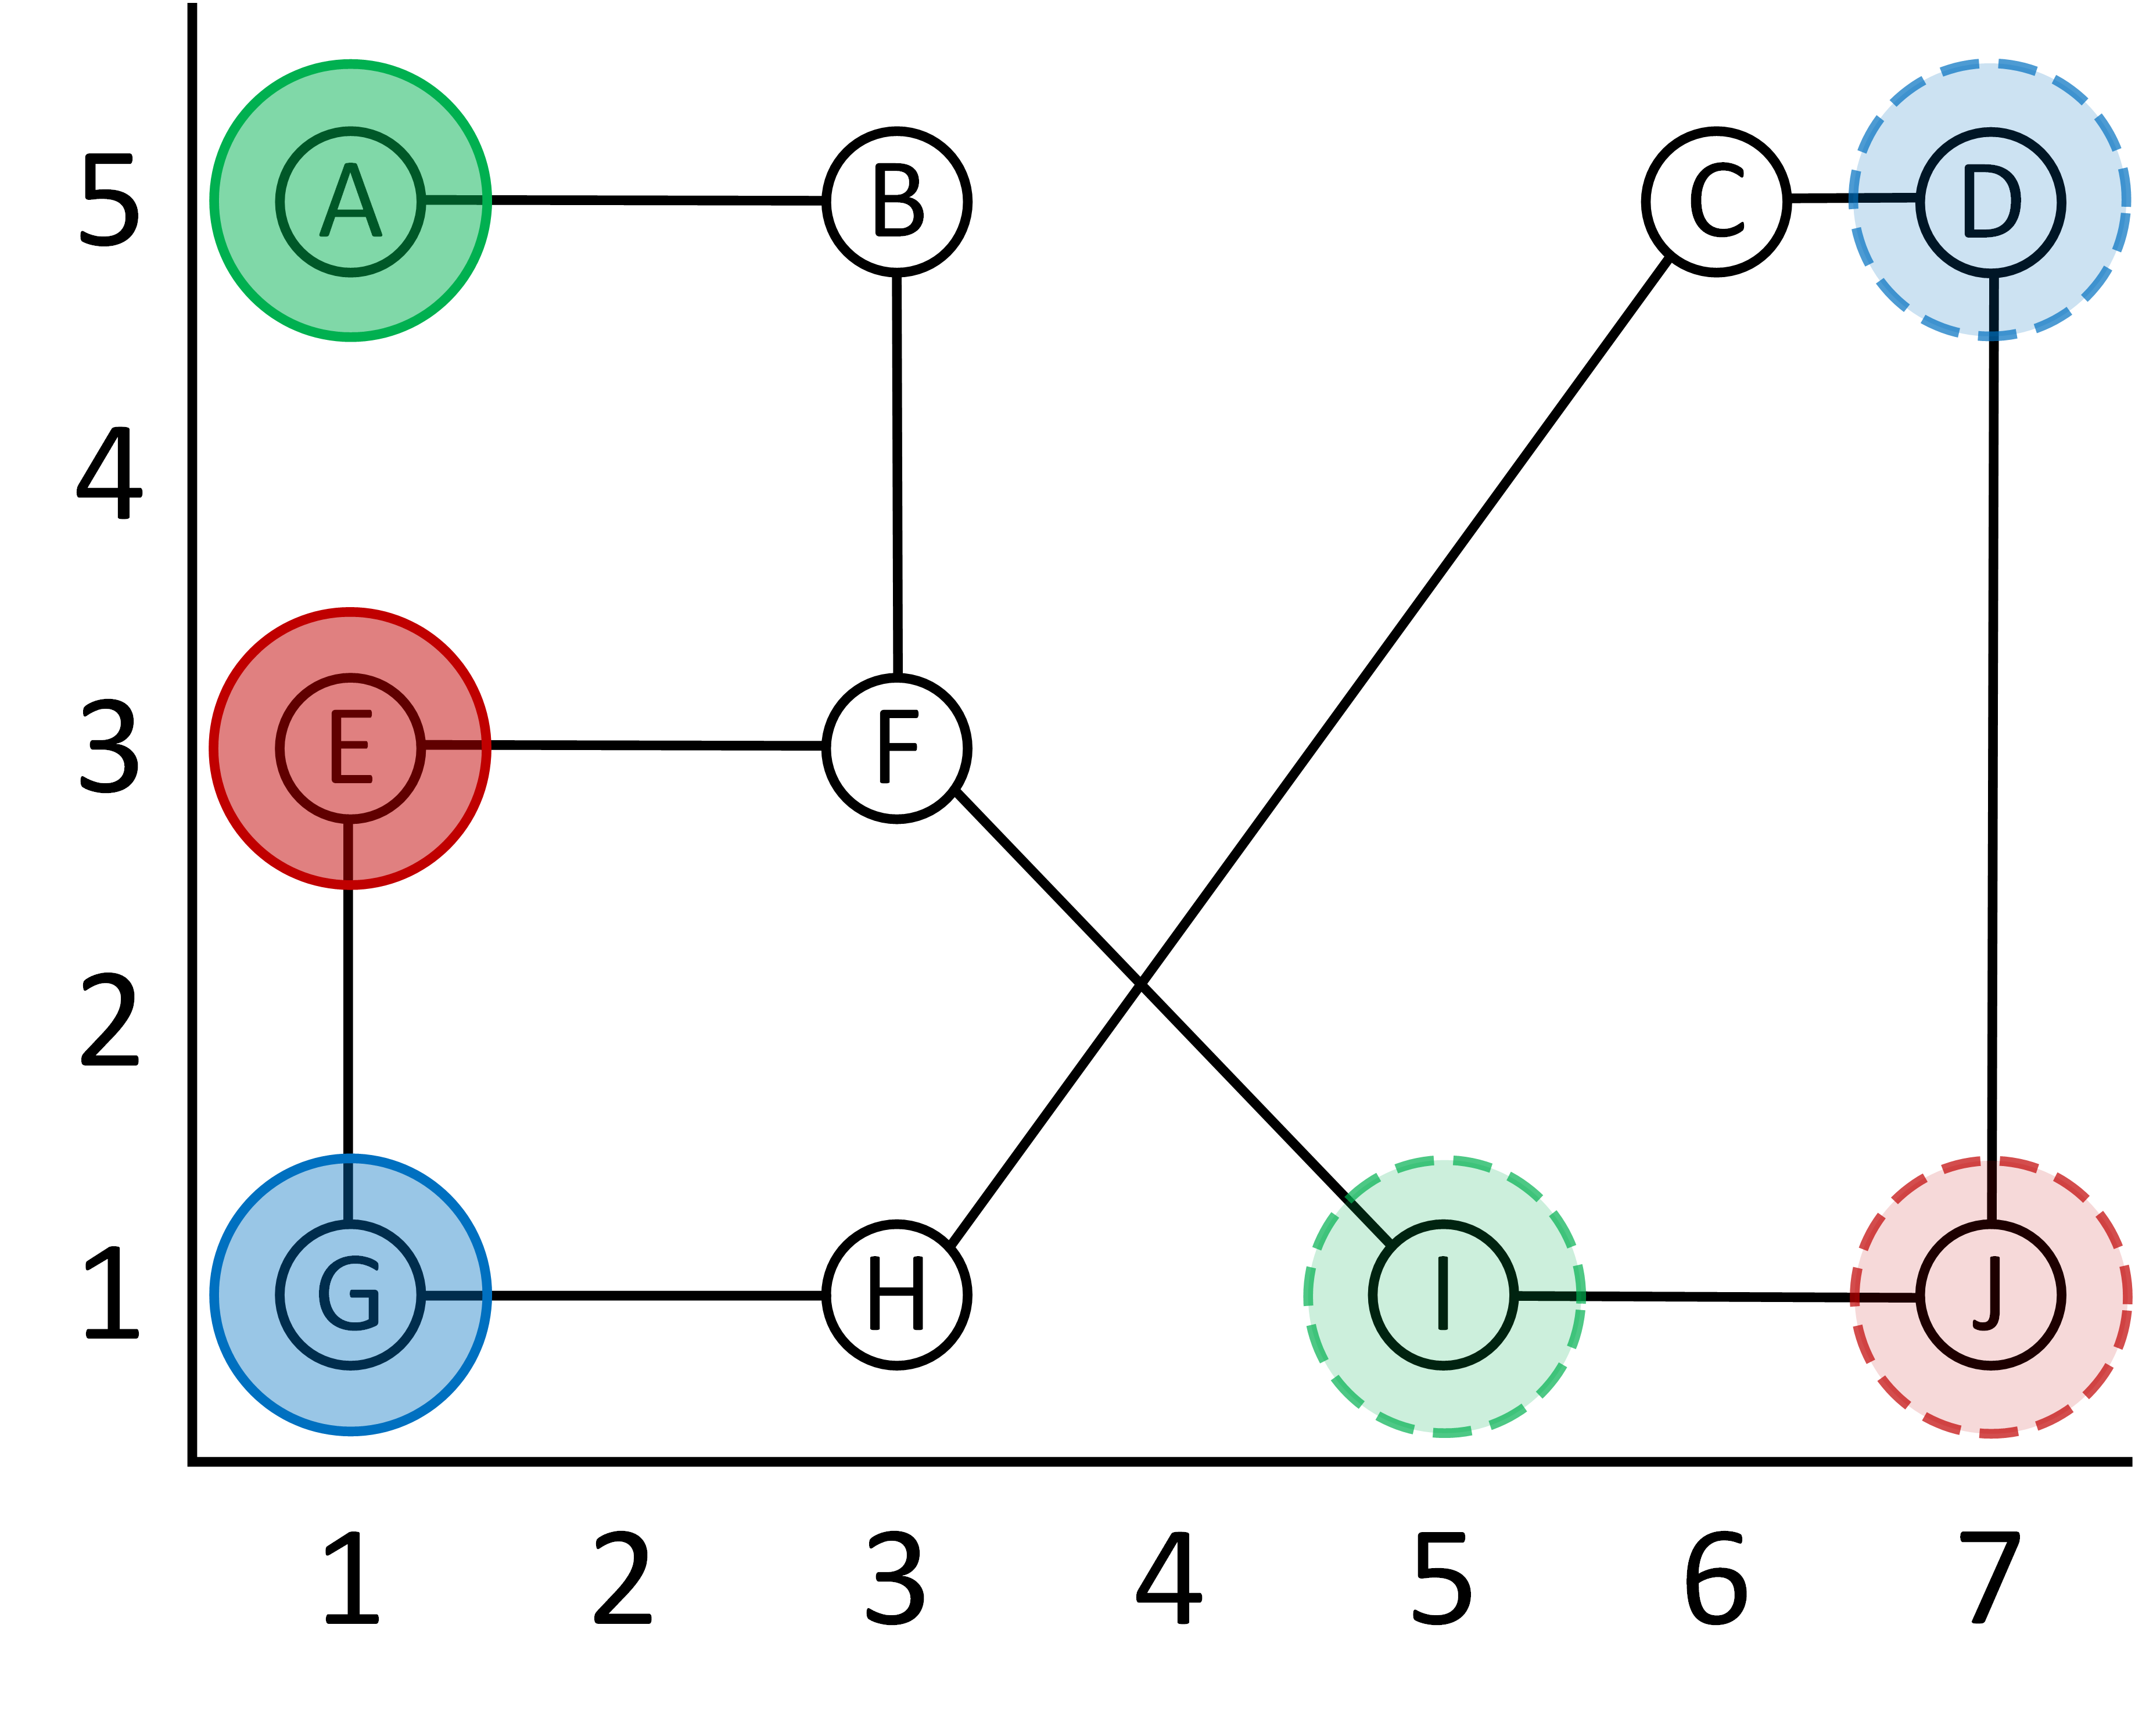
\includegraphics[width=0.6\columnwidth]{running_example.png}
    \caption{A \mapfr problem with 3 agents. The dashed circle mark the goal location of each agent.}
    \label{fig:example}
\end{figure}

\begin{figure}
    \centering
    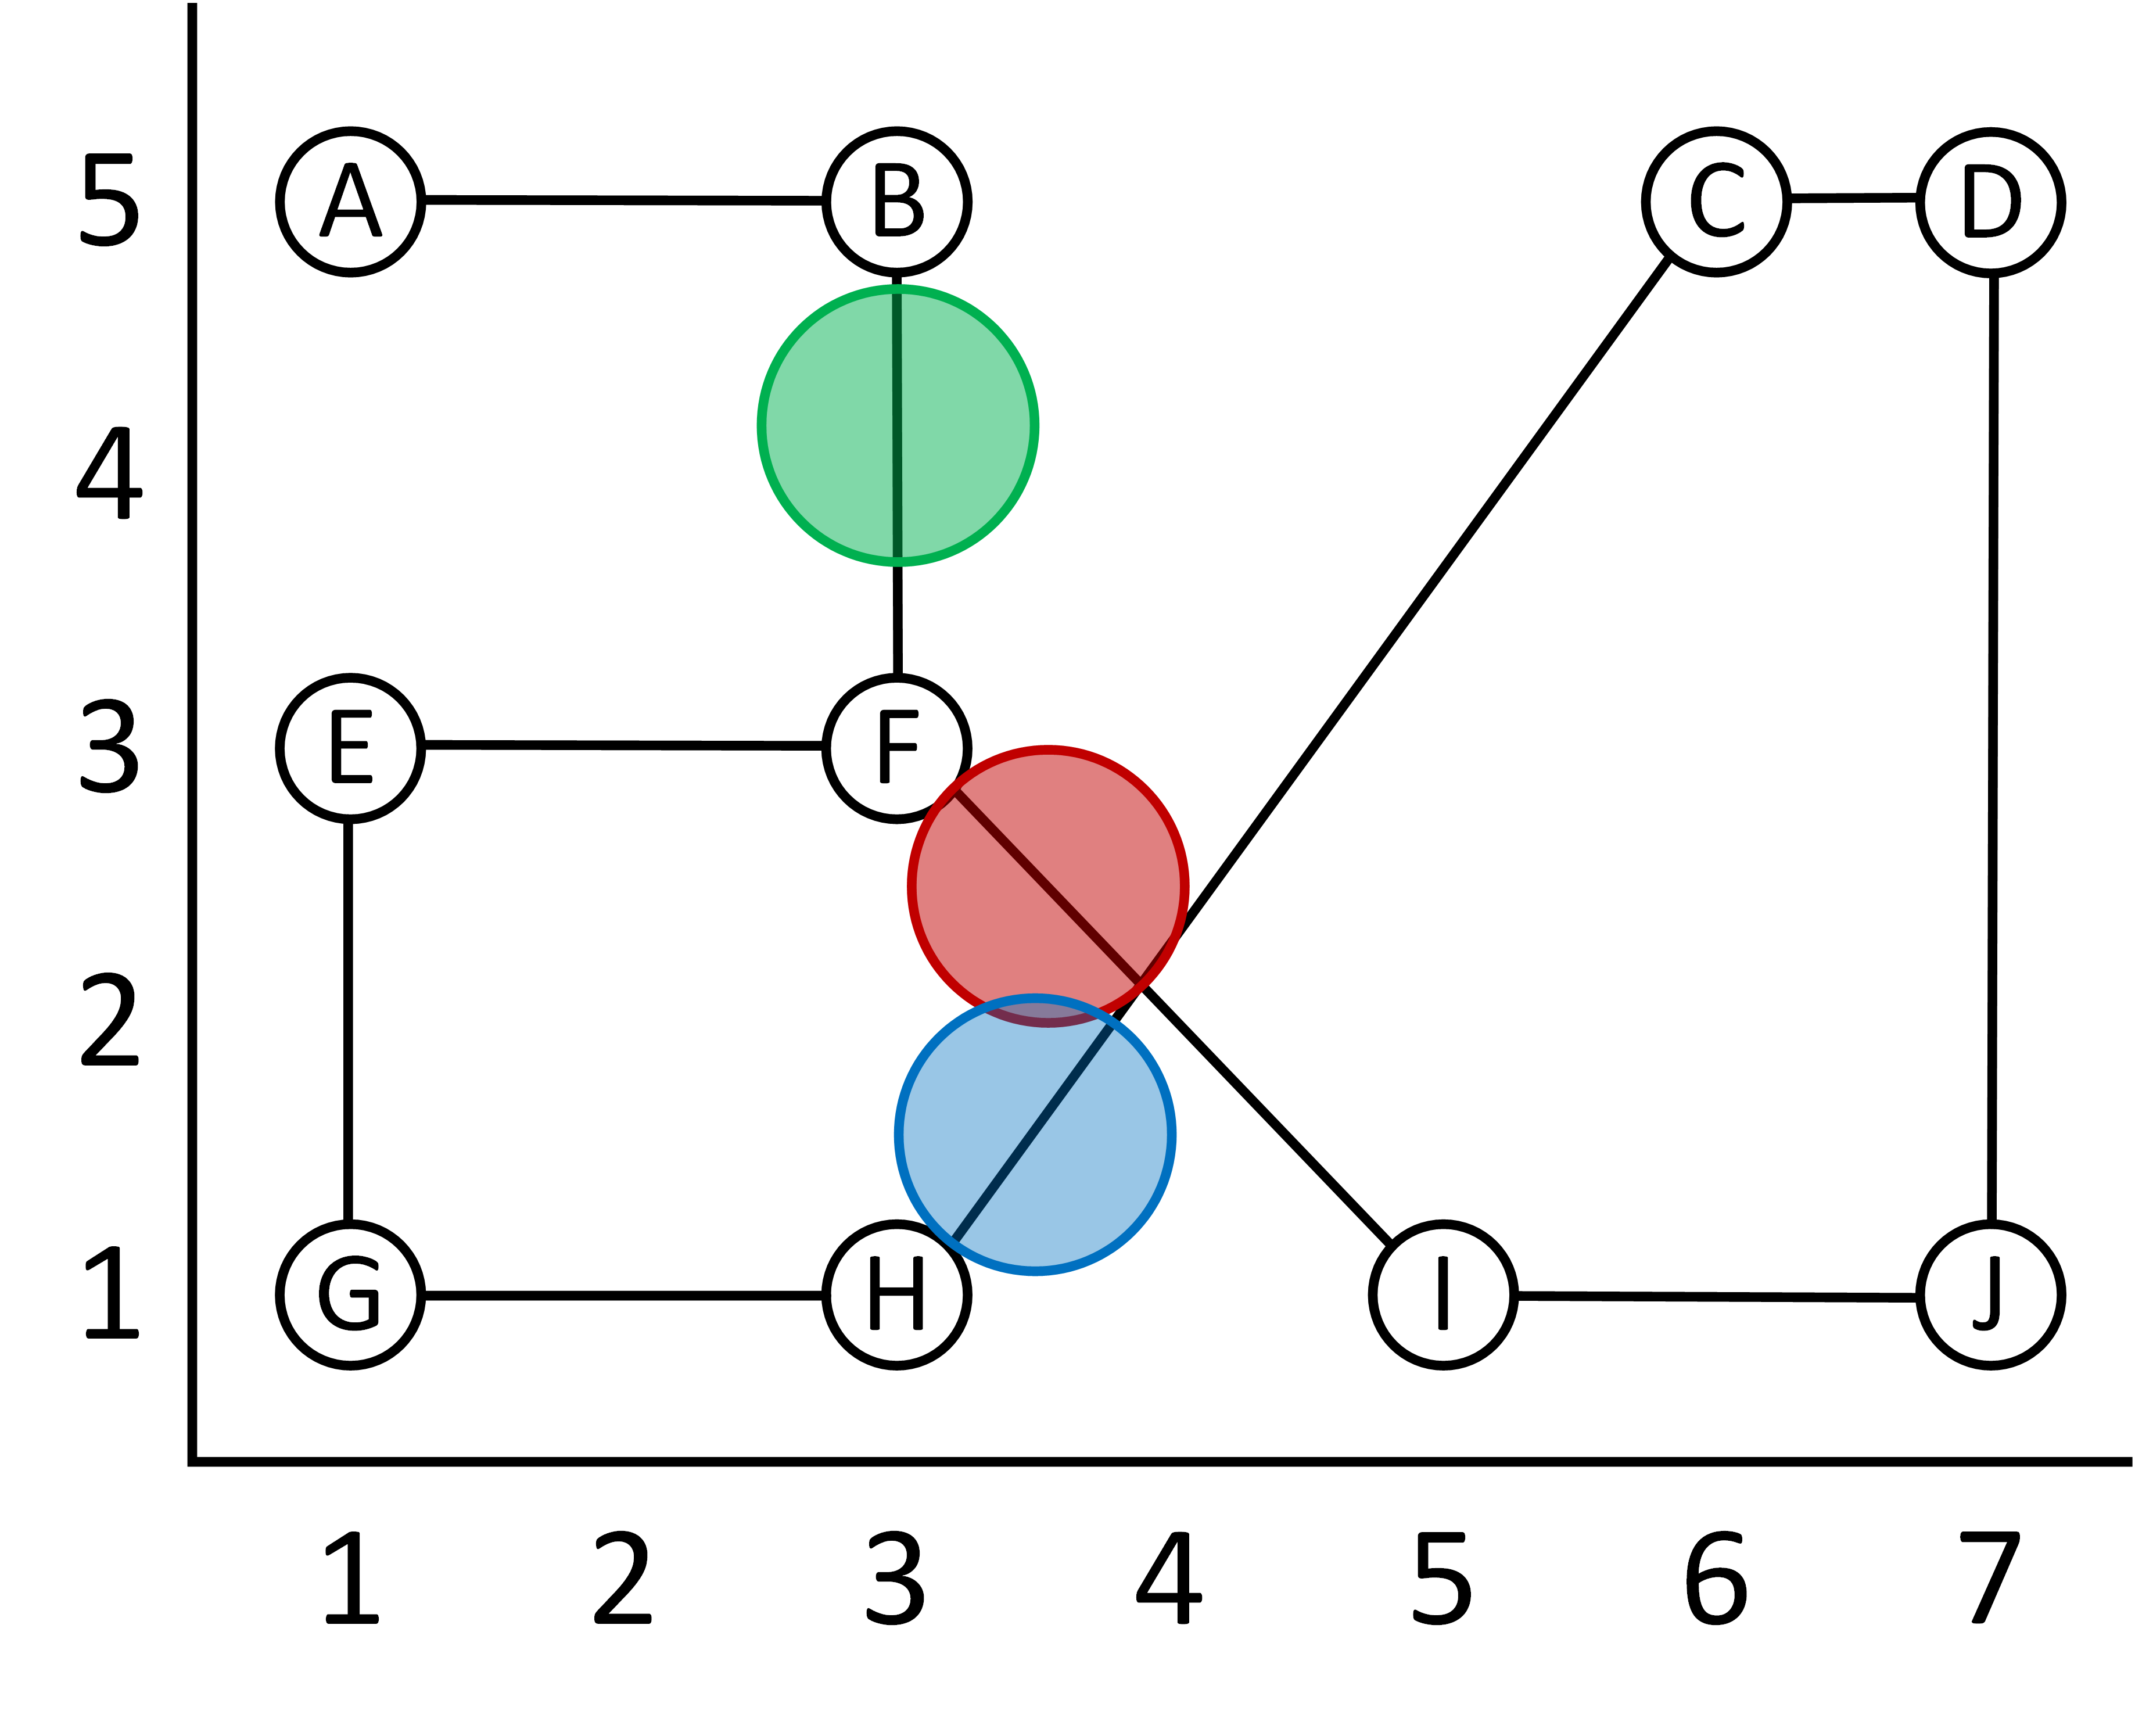
\includegraphics[width=0.6\columnwidth]{running_example_t2-8.png}
    \caption{The positions of the agents at time moment $t=2.8$ when following their individual plans. Red and blue agents are in a collision.}
    \label{fig:example-t-2-8}
\end{figure}

\subsection{\mapfr Example}
Figure \ref{fig:example} shows an example of \mapfr problem. 
Small circles with the letters inside them denote graph vertices, e.g. vertex $A$ corresponds to a point with the coordinates $(1, 5)$, straight line segments between vertices depict edges. %, e.g. vertex $C$ is reachable from $H$ by following the segment that starts at $(3, 1)$ and ends at $(6,5)$. 
Agents are shown as colored circles. Each agent is a disk with a radius of 0.5. Initially the green agent occupies vertex $A$, the red agent -- vertex $E$, and the blue agent -- vertex $G$. Their respective goals are $I$ (green agent), $J$ (red agent), and $D$ (blue agent).

20 move actions, corresponding to 10 undirected graph edges are present in this setting. Assume the agents' moving speed is one; they start and stop instantaneously; and move from one vertex to the other following the straight line segment connecting them. Thus, the duration of every action equals the distance between the vertices that define that move action. E.g. the duration of the action ``move from $A$ to $B$'', denoted as $A \rightarrow B$, is 2. The motion function that describes this action is: $(A \rightarrow B)_\varphi(t) = \overrightarrow{OA} + {1\over{||AB||}} \cdot \overrightarrow{AB} \cdot t$.

The least-cost individual plans to the agents' respective goals are: $\pi_{green}=\{A \rightarrow B, B \rightarrow F, F \rightarrow I\}$ for the green agent; $\pi_{red}=\{E \rightarrow F, F \rightarrow I, I \rightarrow J\}$ for the red agent; $\pi_{blue}=\{G \rightarrow H, H \rightarrow C, C \rightarrow D\}$ for the blue one. If the agents start executing them simultaneously, then at $t=2.8$ their positions will be $(3, 4.2)$, $(3+0.4\cdot \sqrt{2}, 3-0.4\cdot \sqrt{2})$, $(3.48, 1.64)$  respectively (see Figure \ref{fig:example-t-2-8}). The distance between the positions of red and blue agents is less that the sum of their radii, thus, they are colliding and their plans are in conflict. 

%Our aim is to avoid collisions between the agents by finding plans that are conflict-free. In this work we strive for sum-of-costs (or makespan) optimal solutions.
%[[Roni: removed this following our discussion]] \konstantin{Need to check the last sentence in the paragraph above after we finalize problem statement.}\roni{The above part repeats what was said. This is an exmaple, not a problem definition. We have the problem definition above. 


%The least-cost individual plans to the agents' respective goals are: $\pi_{green}=\{(A \rightarrow B, 0), (B \rightarrow F, 2), (F \rightarrow I, 4)\}$ for the green agent; $\pi_{red}=\{(E \rightarrow F, 0), (F \rightarrow I, 2), (I \rightarrow J, 2+2\sqrt{2})\}$ for the red agent; $\pi_{blue}=\{(G \rightarrow H, 0), (H \rightarrow C, 2), (C \rightarrow D, 7\}$ for the blue one. If the agents start executing them simultaneously, then at $t=XXX$ their positions will be $(X, Y)$, $(X, Y)$, $(X, Y)$  respectively (see \ref{fig:example-t-X}). The distance between the positions of $X$ and $Y$ is less that the sum of their radii, thus, they are colliding, thus their plans are in conflict. Our aim is to avoid collisions of the agents by finding plans that are conflict-free. In this work we strive for sum-of-costs (or makespan) optimal solutions.



%\roni{The above: we need to change $G$ in the figure to avoid confusion with the goal function.}
%\konstantin{I think this will ruin some figures Pavel already made. We also have a figure (see. '$running\_example\_tree$' that is dependent on the graph vertex 'G'. May be we keep it as is for now (at least for the initial submission)? }
%\roni{Yes, not important.}


\section{Conflict-Based Search with Continuous Time}
\label{sec:ccbs}
% COPY AND PASTE FROM WORKSHOP PAPER
In this section, we introduce \ccbs{} -- an algorithm that finds SOC-optimal solutions to  \mapfr. 
It is based on two algorithms: \cbs~\cite{sharon2015conflict} and \sipp~\cite{phillips2011sipp}. 
For completeness, we provide a brief relevant background on \sipp before introducing \ccbs. 
%\konstantin{Didn't we want to give a background on CBS as well? I think we had such text at some stage. Why did we marked it out?}\roni{It was moved to the background section.}


\subsection{\sipp}
\sipp~\cite{phillips2011sipp} is a powerful algorithm for building a plan for a single agent moving among static and dynamic obstacles~\cite{phillips2011sipp}. 
It has also been used within prioritized \mapf solvers \cite{yakovlev2017anyAngle} and for solving multi-agent pickup and delivery (MAPD) problems \cite{ma2019lifelong}. 
%and later enhanced in the works \cite{}, \cite{}. 
%In this work we use SIPP as a single-agent planner inside the CBS framework, however it can also be used within prioritized MAPF solvers \cite{yakovlev2017anyAngle}, for solving Multi-agent Pickup and Delivery problems \cite{ma2019lifelong}, etc.
\sipp accepts as input a graph, a start and goal vertices in that graph, and trajectories specifying the motion of the dynamic obstacles over time. 
The algorithm pre-processes these trajectories to compute \emph{safe intervals} for each vertex in the graph. 
A safe interval is a contiguous period of time for a vertex, during which if the agent occupies that vertex then it will not collide with any dynamic obstacle. 
Safe intervals are assumed to be maximal, i.e. extending a safe interval is not possible.

For example, consider a case where only one dynamic obstacle is present and both an agent and the obstacle are disks of radius $r$.
Now, consider a vertex $v$ such that the distance between this obstacle and $v$ is less than $2r$ between time moments $t_1$ and $t_2$. The corresponding safe intervals for $v$ are $[0, t_1]$ and $[t_2, +\infty)$.
Note that in this example, we assume that (1) a collision happens only when the distance between two disks is less than the sum of their radii, when the distance is equal to it -- no collision happens; and (2) the collision does not occur at the specific point $t_1$ and $t_2$.

A vertex may have multiple, non-overlapping, safe intervals. 
In general the number of safe intervals is proportional to the number of the obstacles that pass nearby the vertex. The chronologically last safe interval for a vertex might not end with $\infty$. For example, an obstacle may come to that vertex and stay in it. The safe interval might be an $\emptyset$ as well -- consider e.g. an obstacle that constantly moves back-and-forth in the vicinity of the vertex. 



\sipp performs an \astar-like search over the search space in which each node is a pair of graph vertex and one of its safe intervals. This means there may be multiple search nodes for the same vertex but with different safe time intervals. In the example above, nodes
%$n_1=\langle v, [0, t_1] \rangle$ and $n_2=\langle v, [t_2, +\infty) \rangle$ 
$n_1=(v, [0, t_1])$ and $n_2=(v, [t_2, +\infty) )$ 
correspond to the same vertex $v$, but have different safe intervals.
Guided by a consistent heuristic, \sipp is guaranteed to return optimal solutions. 
Sub-optimal and anytime variations of the algorithm are also known \cite{narayanan2012anytime,yakovlev2020revisiting}. %, but in this work we use the basic, optimal, \sipp. 

%Next we describe the main ideas of SIPP. Without the loss of generality we will consider both the agent and the obstacles to be disks of the same size (radius equals $r$).
%The crux of the method is the notion of the safe interval for a graph vertex~\cite{phillips2011sipp}. The latter \dor{Out of whom?} is a contiguous period of time for a vertex, during which no collision happens with the dynamic obstacles if an agent occupies the vertex. Safe intervals are opposed to collision intervals, and are assumed to be maximal, i.e. extending a safe interval is not possible.


%For each node in its search space, \sipp maintains a $g$-value -- the cost of the best-known plan that ends at this vertex, an $h$-value -- a heuristic estimate of the cost to the goal, $parent$ -- the predecessor node in the search-tree, and the earliest possible time within the safe interval the node can be reach from $parent$. In the considered domain, $g(n)$ and $EAT(n)$ are equivalent as the cost of a plan is the time the agent needs to execute it. Earliest possible arrival time for a node is computed when its predecessor is expanded. Being a planning algorithm, \sipp assumes that the exact procedure of computing this time moment is available.\roni{What is this time moment? not clear} 



\subsection{From \cbs to \ccbs}

\pavel{Why we do not have original CBS pseudo-code to see the difference of CCBS and CBS? I know that I often go back to this question. Not extremely important. We can see difference of CBS and CCBS then.}

\ccbs follows the \cbs framework. %: it has a low-level search algorithm that finds plans for individual agents, and a high-level search algorithm that imposes constraints on the low-level search.
The main differences between \ccbs and \cbs are:
\begin{itemize}
    \item To detect conflicts, \ccbs uses the given conflict detection mechanism $\inconflict$, which, in turn, uses the given geometry-aware collision detection mechanism $\iscollision$. 
    
    %To detect conflicts, \ccbs uses the given, geometry-aware conflict detection mechanism $\iscollision$. \konstantin{Well. Now we have both 'isCollision' and 'inCoflict'. It looks like the later is more suitable here. My version: To detect conflicts, \ccbs uses the given conflict detection mechanism $\inconflict$ (which, in turn, uses the given geometry-aware collision detection mechanism $\iscollision$}
    
    \item To resolve conflicts, \ccbs uses a geometry-aware \emph{unsafe-interval detection mechanism}.
    %\item Conflict detection in \cbs, being trivial, is considered to be part of the algorithm, while conflict detection in \ccbs is considered to be performed by the auxiliary procedure that takes the agents shapes, sizes, kinematics etc. into account. In the considered case of translating disks \ccbs relies on a geometry-aware collision detection procedure.   \roni{This is a too-long discussion at this point.}
    \item \ccbs adds constraints over pairs of actions and time ranges, instead of location-time pairs.
    \item For the low-level search, \ccbs uses a version of \sipp adapted to handle \ccbs constraints. %its unique form of constraints. %a pathfinding algorithm is used that considers continuous time and agents' shape. 
    
%    Instead of imposing constraints over location-time pairs, \ccbs imposes    collision detection mechanism. 
%    \item To resolve conflicts, \ccbs imposes constraints over action-time pairs instead of location-time pairs.
\end{itemize}
\noindent Next, we explain these differences in details. 



\subsubsection{Conflict Detection in \ccbs}

\ccbs is designed for \mapfr, where agents can have any geometric shape, agents' actions can have any duration, and agents move continuously in time following some motion function.
Thus, conflicts can occur between agents traversing different edges, 
as well as between agents where one is traversing an edge and the other is waiting at a vertex~\cite{li2019multi}. 
Also, an action $a$ initiated at some time $t$ may conflict with an action $a'$ initiated at some other time $t'$, as long as there is some overlap in their execution time, i.e., as long as 
$[t,t+a_D]\cap [t',t'+a'_D]\neq\emptyset$. To this end, we define a \ccbs conflict with respect to a pair of \emph{timed actions}.

A timed action is a pair $(a,t)$ where $a$ is an action and $t$ is a point in time. 
To execute a timed action $(a,t)$ means to execute action $a$ starting from time $t$. 
% What is a CCBS conflict 
A \ccbs conflict is a tuple $\tuple{i,j, (a_i, t_i), (a_j, t_j)}$, representing that if agent $i$ executes the timed action $(a_i,t_i)$ and agent $j$ executes the timed action $(a_j,t_j)$ then they will collide. Formally:
\begin{definition}[\ccbs Conflict]
$\tuple{i,j, (a_i, t_i), (a_j, t_j)}$ is a \ccbs conflict, denoted 
$\inconflict \Big(i,j, (a_i,t_i), (a_j,t_j)\Big)$,
iff 
\begin{equation}
\exists t\in [t_i,t_i+{a_i}_D]\cap [t_j,t_j+{a_j}_D]: 
    \iscollision(i,j,{a_i}_\varphi(t-t_i), 
                        {a_j}_\varphi(t-t_j))
\label{eq:inconflict}
\end{equation}
\label{def:ccbs-conflict}
\end{definition}
%We say that $\inconflict \Big(i,j, (a_i,t_i), (a_j,t_j)\Big)$ is true iff Equation~\ref{eq:inconflict} holds. 
Whenever $i$ and $j$ are clear from the context, we omit them and use $\iscollision(m_i,m_j)$ and $\inconflict((a_i,t_i), (a_j,t_j))$. 
Observe that 
a \ccbs conflict is agnostic to the absolute time the actions are performed, and only considers their relative time, that is, for any $\Delta>0$, 
\begin{equation}
    \inconflict((a_i,t_i)(a_j,t_j))\rightarrow
    \inconflict((a_i,t_i+\Delta)(a_j,t_j+\Delta))
    \label{eq:delta-invariance}
\end{equation}


The complexity of computing \inconflict depends on the shapes of the agents $i$ and $j$ and the motion functions of the actions $a_i$ and $a_j$. For the setting used in our experiments -- disk-shaped agents moving in constant speed on straight lines -- we used a fast closed-loop collision detection mechanism~\cite{guy2015} that runs in $O(1)$. 
%\roni{Konstantin, is this correct?} \konstantin{Yes}
In general, computing \inconflict for arbitrary agents' shapes and motion functions translates to the task of collision detection for arbitrary-shaped moving objects, which is a non-trivial problem extensively studied in computer graphics, computational geometry, and robotics~\cite{jimenez20013d}. 


% CCBS conflicts between plans
Any single-agent plan $\pi = (a_1,\ldots, a_n)$ can also be viewed as a set of timed actions $\big\{ (a_1,t_1),\ldots,(a_n,t_n) ,(a_{n+1},t_{n+1}) \big\}$, where $t_i$ is the time in which $a_i$ is planned to be executed according to $\pi$. 
$t_1$ is equal to zero, and for all other values of $i=2,\ldots, n$ it is the duration of the plan up to action $i$, that is, $t_i=(\pi[:(i-1)])_D$. 
The last timed action $(a_{n+1}, t_{n+1})$ is a ``dummy'' wait action whose duration is infinite. The purpose of this last timed action is to detect conflicts between an agent that finished its plan and other agents. 
%\roni{I think this is now correct}
In \ccbs, we say that single-agent plans $\pi_i$ and $\pi_j$ for agents $i$ and $j$ have a \ccbs  conflict if there exists a pair of timed actions $(a_i,t_i)\in \pi_i$ and $(a_j,t_j)\in \pi_j$ such that $\inconflict \Big((a_i,t_i), (a_j,t_j)\Big)$ is true. 
It is straightforward to see that a pair of single-agent plans 
have a conflict, as defined in Definition~\ref{def:conflict-mapfr},
if they have a \ccbs conflict.


In our running from Figure~\ref{fig:example}, consider the following single-agent plans for the green, red, and blue agents, represented as sequences of timed actions:  $\pi_{green}=\{(A \rightarrow B, 0), (B \rightarrow F, 2), (F \rightarrow I, 4)\}$, $\pi_{red}=\{(E \rightarrow F, 0), (F \rightarrow I, 2), (I \rightarrow J, 2+2\sqrt{2})\}$, $\pi_{blue}=\{(G \rightarrow H, 0), (H \rightarrow C, 2), (C \rightarrow D, 7\}$. The plans of the red and blue agents do, indeed, conflict (as was shown on Figure~\ref{fig:example-t-2-8}. \ccbs conflict here is: $\tuple{red, blue, (F \rightarrow I, 2), (H \rightarrow C, 2)}$.  


%\begin{lemma} A pair of single-agent plans $\pi_i$ and $\pi_j$ for agents $i$ and $j$ have a conflict (as defined in Definition~\ref{def:conflict-mapfr}) iff there exists a pair of timed actions $(a_i,t_i)\in \pi_i$ and $(a_j,t_j)\in \pi_j$ such that $\inconflict \Big(i,j, (a_i,t_i), (a_j,t_j)\Big)$ is true.  \label{lem:timedConflicts} \end{lemma}




%To define a \ccbs conflict in a more formal way, assume without loss of generality that $t_i\leq t_j$ and let $\Delta_T=t_j-t_i$. Note that the overlap in time of the timed actions $(a_i, t_i)$ and $(a_j,t_j)$ is the time range $[t_j, t_j+\min({a_i}_D-\Delta_T, {a_j}_D)]$. A pair of timed actions $(a_i, t_i)$ $(a_j, t_j)$ performed by agents $i$ and $j$ has a conflict iff there exists $t$ in the time range $[0, \min({a_i}_D-\Delta_T, {a_j}_D)]$  such that $\iscollision(i,j, {a_i}_\varphi(t+\Delta_T), {a_j}_\varphi(t))$ is true. 
%We overload the \isconflict notation to apply also for timed actions, i.e., $\isconflict \Big(i,j, (a_i,t_i), (a_j,t_j)\Big)$ is true iff the corresponding timed actions of agents $i$ and $j$ have a conflict. 
%\konstantin{I think its a tricky moment: collision detection between shapes at some locations and collision detection between shapes following some motion function is two different things. The latter is more complex than the former.} 
%\roni{Changed the term and a bunch of text to clarify distinction and overall improve }
%\konstantin{I think its def. much better now}



%Regardless, \ccbs as a MAPF algorithm is agnostic to the exact collision detection procedure used. %which should be chosen appropriately taking into account agents shapes and assumptions on kinematics and dynamics. For the considered case of translating circular agents we chose one of the best-known collision detection procedures as described later in Section 4.

%Collision detection for arbitrary-shaped moving objects is a standalone, non-trivial problem extensively studied in computer graphics, computational geometry and robotics. \ccbs as a MAPF algorithm is agnostic to the exact collision detection procedure which should be chosen appropriately taking into account agents shapes and assumptions on kinematics and dynamics. For the considered case of translating circular agents we chose one of the best-known collision detection procedures as described later in Section 4.



%[[Roni: they already did this in MCCBS, so we can't claim novelty on this]]
%\begin{definition}[\ccbs Conflict] A \ccbs conflict w.r.t. a pair of plans $\pi_i$ and $\pi_j$ is defined by a tuple $\tuple{a_i, t_i, a_j, t_j}$,  representing that if agent $i$ executes $a_i$ at time $t_i$  and agent $j$ executes $a_j$ at time $t_j$ then they will collide.  \label{def:ccbs-conflict} \end{definition}

%\roni{Maybe to add that Li et al. also defined a vertex conflict, but it is subsumed by only looking at action conflicts}
%This means that agents may conflict even if they do not occupy the same vertex/edge at the same time. For example, consider the graph depicted in Figure~\ref{fig:conflict}. Agents $i$ and $j$ occupy locations $A$ and $C$. If at the same time $i$ moves along the edge $AD$  and $j$ moves along the edge $CB$, then a collision will occur. Such a ``criss-cross'' conflict is not considered in standard \cbs.

%Since actions in standard \cbs implementation have unit duration, identifying conflicts is relatively straightforward: iterate over every time step $t$ and check if there is a vertex (or an edge) that more than one agent is planning to occupy in time $t$. By contrast, in \ccbs actions can have any duration and thus iterating over time steps in meaningless. 

% KONSTANTIN LOOK HERE
%Also, \ccbs considers the shape agents. This means that agents may conflict even if they do not occupy the same vertex/edge at the same time. For example, consider the graph depicted in Figure~\ref{fig:conflict}. Agents $i$ and $j$ occupy locations $A$ and $C$. If at the same time $i$ moves along the edge $AD$  and $j$ moves along the edge $CB$, then a collision will occur. Such a ``criss-cross'' conflict is not considered in standard \cbs.  


%. There are standard methods to do this by  analyzing the geometric properties of the agents' movement and shape~\cite{guy2015}. %, while others apply  techniques based on time discretization~\cite{todo}.\roni{@Konstantin: maybe you can fill some references for the above?}  
%\ccbs is agnostic to the particular collision detection mechanism that is used. 
%\begin{figure}
%    \centering
%    \includegraphics[width=0.6\columnwidth]{criss-cross.PNG}
%    \caption{An example of a conflict between different edges.}
%    \label{fig:conflict}
%\end{figure}
%\subsubsection{Imposing Constraints to Resolve Conflicts in \ccbs}

\subsubsection{Resolving Conflicts in \ccbs}
% Unsafe intervals
The high-level search in \ccbs runs a best-first search like  \cbs for classical \mapf. In every iteration, a leaf node $N$ in the \ct is selected that has the solution with the smallest cost. 
The $\inconflict$ function is used to check if $N.\Pi$ has a \ccbs conflict. If no \ccbs conflicts were found, $N$ is declared a goal node and the search halts. Otherwise, the high-level search expands $N$ by choosing one of the \ccbs conflicts 
detected in $N.\Pi$. 
Let $\tuple{(a_i, t_i), (a_j, t_j)}$ be that chosen \ccbs conflict. 
\ccbs resolves this conflict by generating two new \ct nodes, $N_i$ and $N_j$. 
To compute the constraints to add to $N_i$ and $N_j$, \ccbs computes for each timed action its \emph{unsafe intervals} w.r.t the other timed action. 
The unsafe interval of $(a_i,t_i)$ w.r.t. $(a_j,t_j)$ is the maximal contiguous time interval starting from $t_i$ in which if agent $i$ will perform $a_i$ then it will conflict with the timed action $(a_j,t_j)$.  
Formally:
\begin{definition}[\ccbs Unsafe Interval]
$[t_i, t^u_i)$ is the unsafe interval for $(a_i,t_i)$ with respect to $(a_j,t_j)$, where
\begin{equation}
    t^u_i = 
    \argmin _{t\in [t_i, t_j + {a_j}_D]}
    \{ \inconflict ((a_i,t),
        (a_j,t_j)) = \false\}
        \label{eq:unsafei}
\end{equation}

and $[t_j, t^u_j)$ is the unsafe interval for 
$(a_j,t_j)$ with respect to $(a_i,t_i)$, where
\begin{equation}
    t^u_j = 
    \argmin _{t\in [t_j, t_i + {a_i}_D]}
    \{ \inconflict ((a_i,t_i),
        (a_j,t)) = \false\}
        \label{eq:unsafej}
\end{equation}

\label{def:unsafe-interval}
\end{definition}


%the unsafe interval for $(a_i,t_i)$ with respect to $(a_j,t_j)$ is $[t_i, t^u_i)$ where
%\begin{equation}
%    t^u_i = 
%    \argmin _{t\in [t_i, t_j + {a_j}_D]}
%    \{ \inconflict ((a_i,t),
%        (a_j,t_j)) = \false\}
%        \label{eq:unsafei}
%\end{equation}

%and the unsafe interval for 
%$(a_j,t_j)$ with respect to $(a_i,t_i)$ is $[t_j, t^u_j)$ where
%\begin{equation}
%    t^u_j = 
%    \argmin _{t\in [t_j, t_i + {a_i}_D]}
%    \{ \inconflict ((a_i,t_i),
%        (a_j,t)) = \false\}
%        \label{eq:unsafej}
%\end{equation}

%\konstantin{Anton pointed out an issue with the above definition of the unsafe interval. Consider that we are talking about unsafe interval of the action $a_i$ w.r.t $a_j$. Now there might not exist a time moment $t$ in $[t_i, t_j + {a_j}_D]$ that \inconflict is $false$, i.e. it is always $true$ in that interval. Conceptually, this means that even if $i$ postpones action $a_i$ for ${a_j}_D$ the actions will still be in conflict. One way of modifying the formula is explicitly adding the case when $\inconflict ((a_i,t_i),(a_j,t))$ is always $true$ in the interval $[t_i, t_j + {a_j}_D]$. In this case $t^u_i = t_j + {a_j}_D$.}
%\konstantin{UPD: After elaboration on that with Anton we agreed that there is no mistake in formulas, defining the endpoints of un-safe interval. The only thing - may be we should mention in text that it might happen that in certain case the endpoint of unsafe interval for $(a_i, t_i)$ w.r.t. $(a_j, t_j)$ is not defined and in this case we need to take action $a_{j+1}$ to define the endpoint.}
%\roni{I think you are referring to the case where the sets in (7) and (8) are empty, and so argmin is not defined. Right? If so, the meaning of this is that there the entire safe interval is unsafe. This means these actions cannot both be performed in their states. That is, the constraints are $\tuple{i, a_i, t_i, t_j+{a_j}_D}$, $\tuple{j, a_j, t_j, t_i+{a_i}_D}$. In some cases, the resulting plans may also have a conflict, but that would be a a conflict with the next action. I add text here below to address this}
If there is no time $t\in[t_i,t_j+{a_j}_D]$ for which $\inconflict((a_i,t),(a_j,t_j))=\false$ then $t_i^u$ is not defined mathematically. 
For such cases, we set $t_i^u$ to be $t_j+{a_j}_D$, indicating that $a_i$ must start after $a_j$ has already finished. Similarly, 
$t_j^u$ can be undefined 
when there is no 
$t\in[t_j,t_i+{a_i}_D]$ for which $\inconflict((a_i,t_i),(a_j,t))=\false$, 
and we set $t_j^u$ to $t_i+{a_i}_D$ in such cases. 

A constraint in \ccbs is of the form $\tuple{i, a_i, [t_i, t^u_i)}$, saying that agent $i$ cannot perform $a_i$ in the range $[t_i,t^u_i)$. When the agent's index is clear from the context, we omit it from the definition of the constraint, i.e., just write $\tuple{a, [t,t^u)}$. 
For a \ccbs conflict $\tuple{(a_i, t_i), (a_j, t_j)}$, \ccbs adds to $N_i$ the constraint $\tuple{i, a_i, [t_i,t^u_i)}$ and adds to $N_j$ the constraint $\tuple{j, a_j, [t_j,t^u_j)}$. 
Section~\ref{sec:conflict-and-unsafe-detection} discusses methods for computing the unsafe intervals. 
%\konstantin{No elaboration on how to compute unsafe intervals is given at this point. This seems strange.}\roni{I think in the current writing it is Ok to leave this for the subsection about this later on.}\konstantin{OK}\roni{Also I say this now explicitly in the text}

% Example
%For example, assume that we are running \ccbs and the high-level search chooses to expand a \ct node in which agent $i$ plans to move along edge $e_i$ at time 5, agent $j$ plans to move along edge $e_j$ at time 5.5, and there is a conflict between these actions, i.e., $\tuple{e_i,5, e_j, 5.5}$ is a conflict. Assume that the duration required to traverse $e_i$ and to traverse $e_j$ is the same. Therefore, the unsafe interval of agent $j$ is smaller than that of agent $i$, because agent $i$ starts earlier and their respective move actions have the same duration. For our example, assume that the unsafe interval for $i$ is $[5,8)$ and for $j$ is $[5.5, 7.5)$.  \ccbs will generate two new \ct nodes: one with the additional constraint $\tuple{i, e_i, [5,8)}$ the other with the additional constraint $\tuple{j, e_j, [5.5,7.5)}$. 

For example, assume that we are running \ccbs over the \mapfr problem depicted in Figure \ref{fig:example}. The high-level search expands a root \ct node that contains individual plans of the agents that were planned agnostic to each other. As mentioned above, the plans of the red and blue agents conflict. This \ccbs conflict is $\tuple{red, blue, (F \rightarrow I, 2), (H \rightarrow C, 2)}$. The unsafe interval of the action $(F \rightarrow I, 2)$ w.r.t. action $(H \rightarrow C, 2)$ is $[2.000,3.743)$, i.e. the first moment of time the red agent might safely start moving from $F$ to $I$ after time $2$ is $3.743$. The unsafe interval of the action $(H \rightarrow C, 2)$ w.r.t. action $(F \rightarrow I, 2)$ is $[2.000,3.310)$.

%\konstantin{Pavel, is it possible for you to compute the exact endpoints of the intervals using the closed-loop formula from your code and present them in the form of $x+y\cdot \sqrt{z}$? In our implementation of CCBS we rely on approximation and can only report approximate endpoints (3.7427 and 3.3099 are, indeed, approximations).}


\subsubsection{\sipp for the \ccbs Low-Level}
The low-level solver of \ccbs is based on \sipp~\cite{phillips2011sipp}. 
Originally, \sipp uses the trajectories of the dynamic obstacles to compute the safe intervals of the graph vertices. In our cases, we do not have dynamic obstacles. Instead, the safe intervals for every vertex is computed by reasoning over the \ccbs constraints passed to \sipp, as follows. A \ccbs constraint $\tuple{i, a_i, [t_i, t^u_i)}$ imposed over a wait action $a_i$ translates to two safe intervals: one that ends at $t_i$ and another that starts at $t^u_i$. 



Consider the following example: two \ccbs constraints imposed over the wait actions associated with the same graph vertex $v$ are passed to \sipp: $\tuple{i, a_1, [t_1, t^u_1)}$ and $\tuple{i, a_2, [t_2, t^u_2)}$ ($t_1 < t^u_1 < t_2 < t^u_2$). Then, the safe intervals for $v$ are the following: $[0; t_1]$, $[t^u_1; t_2]$, $[t_u^2, +\infty)$.\footnote{Note that the safe intervals include the boundary time moments $t_1$, $t_2$. The rationale behind this is the following. \ccbs constrains wait actions that have certain durations, that is -- no wait action is possible that starts at $t_1$ or $t_2$. However, the agent can start moving at $t_1$ (or $t_2$) and thus leave the vertex immediately after that time moment, without violating the \ccbs constraint.}

\ccbs constraints imposed over move actions are incorporated into \sipp in a different way. Let $\tuple{i, a_i, [t_i, t^u_i)}$ be a \ccbs constraint imposed over a move action that is defined by the graph edge $(v, v')$ and a \sipp search node associated with the vertex $v$. 
%$n=\langle v, [t_1, t_2] \rangle$. 
For this search node, we replace the action $a_i$ 
with action $a_i'$ that starts by waiting in $v$ for duration $t^u_i-t_i$ before moving to $v'$.
Formally, $a_i'$ is defined by a duration ${a_i}'_D={a_i}_D+t^u_i-t_i$ and a motion function
\begin{equation}
{a_i}'_\varphi(t)=
\begin{cases}
    \coord(v) & t\leq t^u_i\\
    {a_i}_\varphi(t+t^u_i) & t>t^u_i
\end{cases}
\end{equation}
%\roni{Konstantin, I modified the above. Please check if you like or not}\konstantin{It seems OK. The only thing -- do we need to mention SIPPs interval in text explicitly? It has noting to do with the definition of $a'$ action. May be just say 'and a SIPP search node associated with the vertex $v$?}\roni{I don't fully understand this comment. Go ahead and changea as you see fit, and I'll re-read. } \konstantin{done}

We denote this version of \sipp, which accepts a set of \ccbs constraints, as \csipp. \csipp is similar to Soft Conflict Interval Path Planning (SCIPP) by Cohen et al.~\cite{cohen2019optimal}, which is also a variant of \sipp designed to be a low-level search for \cbs.
%\konstantin{Similar in what sense? That both low-level planners are modifications of SIPP? Well, yes. But conceptually they are different as Liron's SCIPP (as I remember now) imposes constraints not on graph vertexes but rather on cells that are somehow associated with the given MAMP graph. Moreover they somehow impose 'point' constraints. If we want to keep this paragraph, I believe, we should better stress the differences between SCIPP and CSIPP. It might be not an easy task to do :)}
%\roni{I don't see a real problem here. We need to be nice here. I needed a name for our SIPP. They already had a name for their SIPP. Ignoring it is not nice. We don't need to overthink this one. Anyhow, I added a bit more below on the difference}
\csipp and SCIPP are fundamentally different in several aspects. First, SCIPP is designed for the multi-agent motion planning (MAMP) problem addressed by Cohen et al, which is different from \mapfr as explained in Section~\ref{sec:limitations}. 
Second, SCIPP considers constraints over points in time, while CSIPP considers constraints of time intervals. 
Third, SCIPP is designed to consider soft-constraints so as to allow bounded-suboptimal solutions, while \csipp is currently designed to return optimal solutions. 

%whose $g$-value lies in a range $[t_i, t^u_i)$. This corresponds to agent arriving to $v$ in the time range $[t_i, t^u_i)$. Now, when expanding this state and generating the successor, corresponding to moving from $v$ to $v'$, we explicitly prohibit such a move at any time before $t^u_i$, i.e. the minimal $g$-value of the successor might be $t^u_i+a_D$ not $g(n)+a_D$. This corresponds to prohibiting an agent to perform a move action that violates the \ccbs constraint, but rather allowing an agent to wait in $v$ before $t^u_i$ and only then start moving (so no violation of the \ccbs constraint occurs).




%below is the copypaste from the IJCAI'19 paper
%To adapt \sipp to be used as a low-level solver of \ccbs, we modify it so actions that violate the constraints are prohibited. 
%Let $\tuple{i, a_i, [t_i, t^u_i)}$ be a \ccbs constraint imposed over agent $i$. To adapt \sipp to plan for agent $i$ subject to this constraint, we distinguish between two cases: where $a_i$ is a move action and where $a_i$ is a wait action. 

%\noindent \textbf{Move actions.} 
%Let $v$ and $v'$ be the target and destination of $a_i$. 
%If the agent arrives to $v$ in the time range $[t_i, t^u_i)$ then we forbid it from directly moving to $v'$, and add an action that represents waiting at $v$ until $t^u_i$ and then moving to $v'$.  \dor{We already use the term "target". Maybe we should use -- departure and arrival locations.}

%\noindent \textbf{Wait actions.} 
%Let $v$ be the vertex in which the agent is waiting in $a_i$. We forbid the agent from waiting at $v$ in the range $[t_i, t^u_i)$ by splitting the safe intervals of $v$ accordingly. For example, if $v$ is associated with a single safe interval: $[0,\infty)$, then splitting it to two intervals $[0, t_i)$ and $[t^u_i,\infty)$. 

\begin{algorithm}
	\SetKwInOut{Input}{input}
	\Input{$\mathcal{G}=(V,E)$, \source, \target)}
	\ForEach{agent $i$}{
        $\pi_i\gets$\astar$\big(\mathcal{G},\source(i),\target(i)\big)$ \nllabel{line:sipp} \\
        \pavel{Big seems to be something wrong.}
    }
    $N\gets \Big(\emptyset,(\pi_1,\ldots,\pi_k)\Big)$\\
    Create \OPEN; Add $N$ to \OPEN\\
    \While{\OPEN is not empty}{
        $N\gets$ pop $N$ from \OPEN such that
        $\cost(N.\Pi)=\min\limits_{N'\in \OPEN}\cost(N'.\Pi)$ \nllabel{line:pop} \\
        \If{$N.\Pi$ has no conflicts}{
            \Return $N.\Pi$
        }
        $\tuple{i,j, (a_i, t_i), (a_j,t_j)}\gets$ FindConflict($N.\Pi$) \nllabel{line:findconflicts}\\
        \For{$l\in\{i,j\}$ \nllabel{line:ccbs:start-expand}}{
            $[t_l,t^u_l)\gets $ compute unsafe interval for agent $l$ \nllabel{line:unsafe} \\
            $\const \gets N.\const\cup \{
            \tuple{l, a_l, [t_l, t^u_l)} \}$ \nllabel{line:ccbsconstraints}\\ 
           $\pi_l'\gets 
            \csipp\big(\mathcal{G},\source(l),\target(l), \const \big)$\\
            $\Pi'\gets (N.\Pi\setminus \{N.\pi_l\}) \cup \{\pi'_l\}$ \\
            $N_l\gets (\const, \Pi')$\\ 
            Add $N_l$ to \OPEN \nllabel{line:ccbs:end-expand}
        }
    }

\caption{\ccbs pseudo code.}
\label{alg:ccbs}
\end{algorithm}


\subsubsection{\ccbs Pseudo-code}
Algorithm~\ref{alg:ccbs} lists the complete pseudo-code of \ccbs. First, a simple \astar search is used to find a single-agent plan for each agent ignoring all other agents (line~\ref{line:sipp}). Note that \sipp is not needed as this stage, because the optimal plan for each agent at this stage includes only move actions. %\konstantin{I think that in our implementation we use A* for the first pass. There is no point in running SIPP as for every vertex there exist only one maximal safe interval $[0, +\infty)$ at first}\roni{Ok, fixed} 
This set of single-agent plans is used to create the root of the \ct, which is added to the open list (\OPEN). 
Then, in every iteration of the algorithm we extract the node $N$ from \OPEN that has represents a solution with a minimal cost, compared to solutions in the other nodes in \OPEN (line~\ref{line:pop}). 
If $N$ has no \ccbs conflicts, we return $N.\Pi$. 
Otherwise, we choose one of the \ccbs conflicts $C=\tuple{i,j, (a_i,t_i), (a_j,t_j)}$ detected for $N.\Pi$. 
For each agent in the conflict, i.e., $i$ and $j$, we compute the unsafe interval for its action (line~\ref{line:unsafe}), and create a new \ct node with the corresponding constraint and a new single-agent plan for that agent. 
%The corresponding constraints for agent $i$ and $j$ are $\tuple{i,[t_i,t_i^u)}$ and$\tuple{j,[t_j,t_j^u)}$, denoted $C_i$ and $C_j$, respectively.  
Note that in the pseudo-code we use $N.\pi_l$ to refer to the single-agent plan of agent $l$ in $N.\Pi$. This \ct node is added to \OPEN, so that it may be chosen for expansion in future iterations. 


\subsection{Theoretical Properties}

%TODO: Roni


Next, we prove that \ccbs is sound, complete, and optimal. Our analysis is based on the notion of a \emph{sound} pair of constraints, established by Atzmon et al.~\shortcite{atzmon2018robust}. 
%\roni{Dor, you can replace this reference with your newly published JAIR paper!}\dor{Done. :)}

\begin{definition}[Sound Pair of Constraints]
For a given \mapfr problem, a pair of constraints is sound iff in every optimal valid solution it holds that at least one of these constraints hold. 
\label{def:sound}
\end{definition}
 
\begin{lemma}
For any \ccbs conflict $\tuple{(a_i, t_i), (a_j, t_j)}$ 
and corresponding unsafe intervals $[t_i,t^u_i)$
and $[t_j,t^u_j)$, 
the pair of \ccbs constraints 
$\tuple{i,a_i,[t_i,t^u_i)}$ and
$\tuple{j,a_j,[t_j,t^u_j)}$ 
is a sound pair of constraints.
\label{lem:sound}
\end{lemma}
\begin{proof}
By contradiction, assume that there exists a valid solution to the corresponding \mapfr problem 
in which action $a_i$ is performed at time $t_i+\Delta_i\in [t_i,t^u_i)$
and action $a_j$ is performed at time $t_j+\Delta_j\in [t_j,t^u_j)$. This means that
\begin{equation}
    \inconflict((a_i,t_i+\Delta_i),(a_j,t_j+\Delta_j))=\false
    \label{eq:false-assumption}
\end{equation}

\textbf{Case \#1: $\Delta_i>\Delta_j$.} 
By definition, $t_i+\Delta_i-\Delta_j$ is in the unsafe interval $[t_i,t_i^u)$ and therefore:
\begin{equation}
    \inconflict((a_i, t_i+\Delta_i-\Delta_j), (a_j,t_j))
\end{equation}
Due to Equation~\ref{eq:delta-invariance}, this means
$\inconflict((a_i, t_i+\Delta_i),(a_j,t_j+\Delta_j))$, contradicting Equation~\ref{eq:false-assumption}.\\ 

\textbf{Case \#2: $\Delta_j\geq\Delta_i$.}
Similarly, $t_j+\Delta_j-\Delta_i$ is in the unsafe interval $[t_j, t_j+t_j^u)$ in this case, and thus 
\begin{equation}
    \inconflict((a_i, t_i), (a_j,t_j+\Delta_j-\Delta_i))
\end{equation}
Again, using Equation~\ref{eq:delta-invariance} results in 
$\inconflict((a_i, t_i+\Delta_i),(a_j,t_j+\Delta_j))$ which contradicts Equation~\ref{eq:false-assumption}. 
\end{proof}

\begin{theorem}
\ccbs sound, complete, and is guaranteed to return an optimal solution. 
\label{the:optimal}
\end{theorem}
\begin{proof}
Soundness follows from the fact that \ccbs stops only when the $N.\Pi$ has no conflicts. 
Completeness and optimality proof is similar to the completeness and optimality proof for $k$-robust \cbs~\shortcite{atzmon2018robust}, as follows. 

For a CT node $N$, let $\pi(N)$ be all valid \mapfr{} solutions that satisfy $N.constraints$, and let $N_1$, and $N_2$ be the children of $N$. For any $N$ that is not a goal node, the following two conditions hold.
\begin{enumerate}
    \item $\pi(N)=\pi(N_1)\cup\pi(N_2)$
    \item $\cost(N)\leq \min(\cost(N_1.\Pi), \cost(N_2,\Pi))$
\end{enumerate}
The first condition holds because $N_1$ and $N_2$ are constrained by a sound pair of constraints (Lemma~\ref{lem:sound} and Definition~\ref{def:sound}). 
The second condition holds because $N.\Pi$ by construction is the lowest cost solution that satisfies the constraints in $N$, and the constraints in $N_1$ and $N_2$ are a superset of $N.constraints$. 


Now let $N$ be the root of the CT. 
$\pi(N)$ is the set of all valid solutions, 
and thus any valid solution will be either in $\pi(N_1)$ or $\pi(N_2)$. Applying this reasoning recursively yields that every valid solutions is always reachable via one of the un-expanded CT nodes. 
By performing a best-first search over the CT, exploring CT nodes with minimal cost first, \ccbs{} is guaranteed to find an optimal  \mapfr{} solution. 
\end{proof}

%\konstantin{May be we still put the proof here to make the paper self-contained?}
%\roni{Good idea. Dor, can you do this please?}
%\dor{I added a proof, what do you think?}
%\konstantin{My thoughts: 1) I didn't manage to follow the proof of soundness. 2) It looks like only a 'semi-completeness' is proved. I.e. a case when a valid solution to \mapfr does not exist is not considered. Btw, will \ccbs appropriately report 'solution not found' in that case? 3) Do I understand right that this proof says that CCBS is agnostic to objective (SOC or makespan). It will just return an optimal solution in any case?}
%\roni{Re-worded some of the proof. 1) Fixed now. (2) yes, this is correct, added text below (3) yes, pretty cool.}


Note that \ccbs, like \cbs, is complete in a weak way. That is, if a valid solution exists, \ccbs will find it, but if a valid solution does not exists then \ccbs will not detect this. 

% END COPY AND PASTE FROM WORKSHOP PAPER



\subsection{Conflict and Unsafe Interval Detection Methods}
\label{sec:conflict-and-unsafe-detection}


The soundness, completeness, and optimality of \ccbs rely on having accurate collision detection, conflict detection, and unsafe interval detection mechanisms. That is, we require (1) the collision detection mechanism (\iscollision) to detect a collision iff one exists, (2) the conflict detection mechanism to detect a conflict iff one exists (\inconflict), (3) and the unsafe interval detection mechanism returns the maximal unsafe interval for every given pair of actions. 
Constructing such accurate mechanisms for agents with arbitrary shapes and arbitrary motion-functions is not trivial, however for many individual cases there exist fast and exact solutions.

\subsubsection{Implementing Collision Detection}
If the agents are modelled as spheres (or disks in 2D), \iscollision is trivially implemented in $O(1)$ by computing the distance between the centers of the agents and comparing this distance to the sum of their radii. When the agents are convex polyhedrons, \iscollision can be implemented in $O(\log(n) \log(m))$, where $m$, $n$ is the number of vertices comprising the polyhedrons~\cite{dobkin1990determining}. General polyhedra are more difficult to handle. In this case the agents regions or their surfaces are typically decomposed into convex parts and then collision detection is applied to these parts in a systematic fashion, see~\cite{gottschalk1996obbtree} for example.

\subsubsection{Implementing Conflict Detection}
%To implement a conflict detection mechanism, we need to reason about motion over time. 
A general approach to detect conflicts is to sample the agents' motion functions and to apply \iscollision to the sampled positions of the agents. This approach is widespread in robotics, see~\cite{cameron1985study} for example. However, this approach may result in missing conflicts due to inappropriate sampling strategy. To mitigate this issue, more advanced approaches to conflict detection have been proposed -- see Jim{\'e}nez et al.~\shortcite{jimenez20013d} for an overview. 
Tang et al.~\cite{tang2014fast} proposed a particular mechanism that accurately solves conflict-detection queries when the agents are represented as triangle meshes (i.e. their bounding surfaces are composed of triangles whose coordinates are known). These \inconflict detectors are non-trivial to implement and computationally expensive. Fortunately, in a number of cases exact and fast \inconflict implementations can be proposed. For example, when agents are represented as disks that move along straight lines with constant speed, conflict detection can be done in $O(1)$ using a closed-loop formula~\cite{guy2015}. 
Walker and Sturtevant~\cite{walker2019collision} proposed an extension of this formula that is able to handle accelerated movements. 



%There are various ways to detect collisions between agents with volume in a continuous space, including closed-loop geometric computations as well as sampling-based approaches. See Jim{\'e}nez et al.~\shortcite{jimenez20013d} for an overview and \cite{tang2014fast} for an example of particular collision detection procedure. For the constant velocity disk-shaped agents we used in our experiments, there exists a closed-loop accurate collision detection mechanism described in \cite{guy2015}. 

\subsubsection{Implementing Unsafe Interval Detection}

% Computing unsafe intervals
Computing the unsafe interval of an action w.r.t another action also requires analyzing the kinematics and geometry of the agents. However, unlike collision and conflict detection, which have been studied for many years and can be computed with closed-loop formulas in some settings, the problem of computing an unsafe interval is less investigated.  %(presumably, due to the fact that it arises only in limited number of cases, path planning including). \roni{Not sure if this helps}
A na\"ive general method for computing the unsafe interval for an action $a_i$ is to apply the conflict detection mechanism multiple times, starting from $t=t_i$ and incrementing $t$ by some small $\Delta>0$ until  \inconflict returns $false$, meaning the unsafe interval is done. This approach is limited in that the resulting unsafe interval may be larger than the real one. One can extend this approach to get a more accurate solution, as follows. Suppose that \inconflict returns $true$ when the start moment of the action $a_i$ is $t_i + (k-1)\Delta$ and returns $false$ if it is $t_i + k\Delta$. Obviously, the true endpoint of the unsafe interval lies in $(t_i + (k-1)\Delta, t_i + k\Delta]$. One can now apply binary search over this interval to identify the unsafe interval endpoint. Theoretically, this search may not converge due to unlimited number of time moments comprising the interval. However, in practice these moments are represented as the floating-point approximations thus the search will, indeed, converge. Moreover the resultant endpoint will be exact in the sense that a computer program is not able to present this endpoint with more accuracy. Finally, a recent investigation of Walker and Sturtevant~\cite{walker2019collision} describes an approach to compute the ``exact minimum delay for collision avoidance" in case agents are discs moving with constant velocities. This can be straightforwardly transformed to exact computation of the \ccbs unsafe intervals.

Overall, when agents are represented as disks that move from one location to the other with constant velocities along the straight lines, there exist fast and exact mechanisms to implement \iscollision, \inconflict, and to compute the endpoints of unsafe intervals. 


%\roni{Konstantin: are the subsequent paragraphs still relevant?} \konstantin{No. After a number of tests we came to an implementation that is i) as good in terms of success rate as the best implementation from IJCAI-19 (in some settings current version is slightly better (1-3\%), in others - IJCAI-19 one, sometimes they are on par.) ii) is more 'universal' in a sense that we can implement FOCAL-search over the CT-tree with the current implementation. I can describe it, if needed.}
%\roni{OK, commenting them out. Worthwhile, perhaps at the future work section, to mention that one may consider smart conflict heuristics, but our prior work on it did not yield significant gains.}

%\subsubsection{Conflict Detection and Selection Heuristics} As noted above, conflict detection in \ccbs is more complex than in regular \cbs. Indeed, in our experiments we observed that conflict detection took a significant portion of time. To speedup the conflict detection, we only checked conflicts between actions that overlap in time and may overlap geometrically. %In addition, we implemented two heuristics for speeding up the detection process. We emphasize that these heuristics do not compromise our guarantee for soundness, completeness, and optimality. 
%The first heuristic we used, which we refer to as the \emph{\history heuristic}, keeps track of the number of times conflicts have been found between agents $i$ and $j$, for every pair of agents $(i,j)$.  Then, it checks first for conflicts between pair of agents with a high number of past conflicts. When a conflict is found, the search for conflicts is immediately halted. That found conflict is then stored in the CT node, and if that CT node will be expanded then it will generate CT nodes that are aimed to resolve this conflict. This implements the intuition that pairs of agents that have conflicted in the past are more likely to also conflict in the future.
%We have found this heuristic to be very effective in practice for reducing the time allocated for conflict detection. 
% Using this heuristic, however, has some limitations. Prior work has established that to intelligently choosing which conflict to resolve when expanding a CT node can have a huge impact on the size of the CT and on the overall runtime~\cite{boyarski2015icbs}. Specifically, Boyarski et al.~\shortcite{boyarski2015icbs} introduced the notion of \emph{cardinal conflicts}, 
%which are conflict that any way to resolve them will result in increasing the \ac{SOC}. \emph{Semi-cardinal conflicts} are conflicts that resolving them by replanning for one of the involved agents will increases the solution cost, but replanning for the other involved agents do not increase solution cost. 

%For \cbs, choosing to resolve first cardinal conflicts, and then semi-cardinals, yielded significant speedups~\cite{boyarski2015icbs}.  However, to detect cardinal and semi-cardinal conflicts, one needs to identify all conflicts, while the advantage of the heuristic is that we can halt the search for conflicts before identifying all conflicts. 


 %To this end, we proposed a second hybrid heuristic approach. Initially, we detect all conflicts and choose only cardinal conflicts. However, if a node $N$ does not contain any cardinal or semi-cardinal conflict, then for all nodes in the CT subtree beneath it we switch to use the \history heuristic. This hybrid approach worked well in our experiments, but fully exploring this tradeoff between fast conflict detection and smart conflict selection is a topic for future work.


\section{An SMT-Based Approach for Makespan-Optimal \mapfr}
\label{sec:smtccbs}
% What we want: SAT-based for MAPFR \smtcbsO ~ (see Section~\ref{sec:smtcbs}) is able to outperform \cbs in some standard classical \mapf benchmarks~\cite{DBLP:conf/ijcai/Surynek19}, leveraging the power of modern SAT solvers.  In this section, we describe \smtccbs, which follows a similar algorithmic framework. 

%Compiling a classical \mapf problem to Boolean satisfiability (SAT) problem and solving it with an off-the-shelf SAT solver is a well-studied successful alternative to \cbs~\cite{surynek2012towards,surynek14compact,DBLP:conf/ecai/SurynekFSB16,DBLP:conf/ijcai/Surynek19}. In some domains, SAT-based \mapf algorithms may outperform \cbs, e.g., in small densely populated graphs~\cite{surynekFSB16comparison,surynek17expansion,DBLP:conf/ecai/SurynekFSB16,DBLP:conf/ijcai/Surynek19}. 
%Thus, natural question in our context is: can we create an alternative to \ccbs that is based on SAT?

% SAT-based for MAPFR is non-trivial. The world is no longer Boolean. 
%\smtcbsO is based on the same encoding of \mapf to SAT described in Section~\ref{sec:mdd-sat}. It creates Boolean variables  $\mathcal{X}_{v}^{t}(i)$ for every time step $t$ agent $i$ may be at location $v$and Boolean variables $\mathcal{E}_{u,v}^{t}(i)$ for every time step $t$ agent $i$ may move from $u$ to $v$.  Such an encoding cannot be used directly for \mapfr, since in \mapfr there is no notion of time steps as time is continuous. In other words, the number of Boolean variables $\mathcal{X}_{v}^{t}(i)$ and $\mathcal{E}_{u,v}^{t}(i)$ required to solve a \mapfr problem with \mddsat, is infinite. 


% Outline of section
In this section, we present \smtccbs, which is an algorithm that  finds makespan-optimal solutions to \mapfr problems. 
As it name suggests, \smtccbs builds on the \smtcbsO algorithm~\cite{DBLP:conf/ijcai/Surynek19} for classical \mapf . 
It breaks the problem of finding a valid makespan-optimal solution in \mapfr into a sequence of \emph{bounded-cost \mapfr problems}. 
A bounded-cost \mapfr problem is the problem of finding a valid solution to a given \mapfr problem with makespan lower than a given bound $\mu$. 
Each of the bounded-cost \mapfr problems created by \smtccbs are solved using an \smt problem-solving procedure. 
Section~\ref{sec:smt-fixed} describes in details how \smtccbs solves each of these bounded-cost problems 
and Section~\ref{sec:musmtcbs} provides a complete pseudo-code for \smtccbs. 


%A significant difficulty in MAPF$_R$ is that we need decision variables with respect to continuous time. Fortunately we do not need a variable for any possible time but only for important moments derived from CCBS conflict elimination constraints.
%Initially we proceed as in the case of CCBS, that is we search for shortest individual paths for each agent. Decision variables then correspond to vertices/edges and time intervals during which the agents visited and traversed edges.



\subsection{Solving Bounded-Cost \mapfr Problems with \smt}
\label{sec:smt-fixed}
% We use SMT to solve the fixed makespan problem.
%\konstantin{We agreed that we would use \decidemapfr notation when talking about SMT for \mapfr, so I changed text in accordance with that agreement in the subsequent text.}Good.

%The formula satisfiability problem answers yes/no questions. Therefore to find an optimal solution w.r.t. given objective using compilation to satisfiability we need a fixed-objective decision variant of the original problem. Then multiple fixed-objective variants are compiled and answered whether they are satisfiable or not in order to find the optimum.[[Roni: now this is redundant, as it is explained in the background when talking about \smtcbsO]

We refer to the \smt-based bounded-cost \mapfr algorithm we propose as $\mu$\smtccbs. 
Some aspects of $\mu$\smtccbs are similar to the \smt-based bounded-cost \mapf algorithm used by \smtcbsO. 
The propositional skeleton (\ps) in $\mu$\smtccbs is constructed such that a 
satisfying assignment to this \ps defines a solution to $P$ with makespan at most $\mu$, 
where $P$ is the \mapfr problem we are solving. 
The \decidet procedure in $\mu$\smtccbs checks if this solution is valid, i.e., if it contains any \ccbs conflicts. 
We refer to this procedure as to \decidemapfr .
If the solution is not valid, \decidemapfr returns one of the detected \ccbs conflicts. 
Then, the \ps is updated so that assignments that satisfy it 
define a solution in which all the \ccbs conflicts returned so far by \decidemapfr are avoided. 
%This algorithm mimics the behavior of \ccbs in that it detects \ccbs conflicts and resolves them by imposing of \ccbs constraints. 




\begin{algorithm}
	\SetKwInOut{Input}{Input}
	\Input{$P$, the \mapfr problem; $\mu$, the makespan bound}
	$\Psi\gets\emptyset$ \nllabel{line:smt:init}\\
	\While{True}{
	%	(\ps,$\mu_{next}$) $\gets$ CreatePS($\Psi$, P, $\mu$) \nllabel{line:smt:createps}\\
	\ps $\gets$ CreatePS($\Psi$, P, $\mu$) \nllabel{line:smt:createps}\\	
		$\Pi\gets$ Solve(\ps) \nllabel{line:smt:solve}\\
		\If{No solution found (i.e., $\Pi$ is null)}{
		%	\Return ($null$, $\mu_{next}$) \nllabel{line:smt:no-solution}
			\Return $null$ \nllabel{line:smt:no-solution}
		}
		$Con\gets$ \decidemapfr($\Pi$, P, $\mu$) \nllabel{line:smt:decidet}\\
		\If{No conflict found (i.e., $Con$ is null)}{
			\Return $\Pi$ \nllabel{line:smt:solution}
		}
		Add $Con$ to $\Psi$\\
	}
	\caption{The $\mu$\smtccbs algorithm.}
	\label{alg:smt-ccbs}
\end{algorithm}

% Pseudo code
Algorithm~\ref{alg:smt-ccbs} lists a high-level pseudo-code for $\mu$\smtccbs. 
$\mu$\smtccbs maintains a set $\Psi$ that contains all the \ccbs conflicts returned by our \decidemapfr procedure so far. 
Initially, $\Psi$ is empty (line~\ref{line:smt:init}). 
In every iteration of $\mu$\smtccbs, the \ps is created for the current set of conflicts (CreatePS($\cdot$) in line~\ref{line:smt:createps}). 
A SAT solver is used to search for a satisfying assignment to this \ps~ (line~\ref{line:smt:solve}). 
If no solution exists, the given decision problem is unsolvable, i.e., there are no solutions to $P$ with makespan equal to or smaller than $\mu$.  
Otherwise, we apply \decidemapfr to check if the found solution is a valid \mapfr solution (line~\ref{line:smt:decidet}). 
If it is a valid solution, we return it.
Otherwise, \decidemapfr returns one of the \ccbs conflicts that exists in this solution. 
The returned \ccbs conflict is added to the set of conflicts $\Psi$. 
This process continues until either a valid solution is found (line~\ref{line:smt:solution}) or we establish that no solution exists (line~\ref{line:smt:no-solution}).


Our \decidemapfr procedure is exactly the same as the conflict-detection step in \ccbs. 
It applies a conflict-detection mechanism to check for collisions between the agents' plans in the given solution. 
The process of generating our \ps for a given set of \ccbs conflicts, \mapfr problem, and makespan bound -- CreatePS($\Psi$, P, $\mu$) -- is more involved and we describe it next. 




\subsubsection{Generating the Propositional Skeleton}
\label{sec:propositional-skeleton}
%The propositional skeleton in our SMT-based algorithm asks the question: is there a solution to the given fixed-makespan \mapfr problem that is consistent with a given set of \ccbs constraints. We describe how to generate such a propositional skeleton in Section~\ref{sec:propositional-skeleton}. The \decidet


% Introducing MDD_R. High-level
%The objective of the \ps generated for an implicit Constraint Tree \implicitct is to find a solution that satisfies at least one of the \ct nodes in \implicitct. 



% The problem. This somewhat repeats what we have above. Maybe remove?
%The CreatePS procedure accepts a \mapfr problem, a makespan bound $\mu$, and a set of \ccbs conflicts $\Psi$. It outputs a \ps that is satisfiable iff there exists a solution (not necessarily valid) to the given \mapf problem with makespan at most $\mu$ that does not have any of the \ccbs conflicts in $\Psi$. We generate such a \ps by mimicking \ccbs, as follows. 

% Approach: mimic ccbs: define a sound pair of ccbs constraints for every ccbs conflict as defined in Lemma 1. Then simulate csipp. 

%The CreatePS procedure generates a \ps such that a satisfying assignments to itdefines a solution in which all the \ccbs conflicts in $\Psi$ are avoided. 

\noindent CreatePS consists of the following steps. 
\begin{enumerate}
	\item Compute a set of \ccbs constraints for the set of conflicts in $\Psi$. 
	\item Compute for each agent a set of single-agent plans that satisfy these constraints. %\konstantin{Why do we have 'some' here? It introduces some vagueness to the phrase. May be we just cut out 'some'?}\roni{Fixed. Also, now explaining there is a set per agent. I did not want to make this high-level sentence too long, so I did not add ``constraints that are relevant to that agent''. This is also not needed from a correctness perspective: the single-agent plan of one agent always satisfies all constraints of the other agents.}
	\item Create a \ps for choosing a solution from these sets of single-agent plans. %\konstantin{My variant: Create a \ps out of this set of single-agent plans.} \roni{I modified my version a bit and think it is better, as it is more accurate: the \ps allows choosing a solution from the set of solutions specified in the single agent plans we created. Your version says it creates the \ps out of this set, but what does it mean to creat a \ps out of a set? Anyhow, this is not important in my opion, change to however you prefer}
	\item Add constraints to verify the chosen solution avoids all conflicts in $\Psi$. %\konstantin{My variant: extend the \ps with the formulas that correspond to the \ccbs constraints.} \roni{Again, choose what you prefer, but I like my version better because it says what these constraints says, while in your version it seems like this is the only place where the \ccbs constraints are considered, while they are very much considered when generating the \mddr. But, I don't feel strongly about this, choose the option you prefer.}
\end{enumerate}
Next, we describe the details of each step of CreatePS. 
As you will see, these steps are designed to obtain a behavior similar to \ccbs. 
In particular, in the first step, CreatePS computes all the constraints \ccbs would impose to resolve the conflicts in $\Psi$, 
and in the second step, CreatePS computes efficiently all single-agent plans that \csipp would generate to satisfy every subset of these constraints.\footnote{Note that CreatePS does so without explicitly running \csipp an exponential number of times.}


%\textbf{Step \#1. Compute the set of relevant \ccbs constraints.}
\textbf{Step 1. Compute the set of \ccbs constraints for $\Psi$.}
%\konstantin{In the following text I changed $C$ to $Con$ as we used $Con$ in pseudocode.}Good
For every \ccbs conflict $Con$ in $\Psi$, we generate the pair of \ccbs constraints \ccbs would create to resolve $Con$. 
This pair of \ccbs constraints is specified in Lemma~\ref{lem:sound}. 
Note that to compute such a pair of constraints, we need to compute the unsafe intervals for the respective conflict. 
By $\const(Con)$ we denote the pair of \ccbs constraints for a conflict $Con\in \Psi$, 
and by $\const(\Psi)$ -- the set of all pairs of \ccbs constraints were generated this way, i.e., 
\begin{equation}
\const(Con) = \const(\tuple{ (a_i, t_i), (a_j,t_j) }) = \{ \tuple{i, a_i, [t_i, t_i^u)}, \tuple{j, a_j, [t_j, t_j^u)} \}
\end{equation}
\begin{equation}
\const(\Psi) = \{ \const(Con)~|~Con\in \Psi\} 
\end{equation}
%\begin{equation}
%Cnst_i(\Psi) = \{ \tuple{i, a_i, [t_i, t_i^u)} | 
%\exists C\in \Psi ~~ \tuple{i, a_i, [t_i, t_i^u)}\in Cnst(C) \}
%\end{equation}

%\konstantin{Resultant set, $Cnst$, is the 'set of pairs of CCBS constraints', so is it right to name this algorithmic step as 'compute the set of relevant CCBS constraints' and not the 'compute the set of relevant CCBS constraint pairs'?}


\textbf{Step 2. Compute the set of relevant single-agent plans.}
For each agent, we compute all single-agent plans \csipp would generate for that agent given any subset of constraints in $\const(\Psi)$ that involve that agent. 
To compute and store this set of single-agent plans efficiently, we create for each agent a 
specific \emph{Multi-Value Decision Diagram} (MDD)~\cite{srinivasan1990algorithms} that we refer to as \mddr. 
An MDD is a direct a-cyclic graph with a single source and sink.\footnote{Technically, an MDD can have multiple sinks, where each sink is labeled as either true or false. This is equivalent to having a single sink that gathers all sinks labeled as true, and removing all branches that only end up in sinks labeled as false.}
MDDs have been used in the context of \mapf before, e.g., in the ICTS and E-ICTS algorithms~\cite{sharon2013increasing,walker2018extended}. 
Every node in our \mddr is a pair $(u,t)$ where $u$ is a vertex in $\mathcal{G}$ 
and $t$ is a point in time. 
An edge $((u,t)(v,t'))$ corresponds to a timed action from $u$ to $v$ that starts at $t$ and ends in $t'$. We generate our \mddr by performing a variant of Dijkstra's algorithm that considers all possible wait actions \csipp may include to avoid any constraint in $\const(\Psi)$. 
Algorithm~\ref{alg:generate-mddr} describes in details how this is done. 

%Alternative version 3, from the appendinx, now set as final version, other versions commented out
\begin{algorithm}[h!]
\begin{footnotesize}
\SetKwBlock{NRICL}{GenerateMdd$_R$ ($\Pi$, $\const(\Psi)$, $\mu$, i)}{end} \NRICL{
        $X^i \gets \{ (\source(i),0) \}$; $E^i \gets \emptyset$; $\OPEN \gets \emptyset$ \\   
        insert $(\source(i),0)$ into \OPEN \\
        \While {$\OPEN \neq \emptyset$} {
                $(u,t) \gets$ pop $(u,t)$ from \OPEN where $t=\min_t(\OPEN)$\\ % We use this notation of pop throughout the paper
                \If {$t \leq \mu$}{
    	            \ForEach{$a\in \mathcal{A}$ such that $\fromv(a)=u$ and $t+a_D\leq \mu$}{
                 		insert $(\tov(a),t+a_D)$ into $\textsc{Open}$ \nllabel{bla}\\    
             		    
$X^i \gets X^i \cup \{  (\tov(a),t+a_D) \}$ \nllabel{line:generate-mddr:start:move} \\             		 		
$E^i \gets E^i \cup \{  [(u,t);(\tov(a),t+a_D)] \}$ \nllabel{line:generate-mddr:end:move} \\             		 						
                			%\ForEach{$\tuple{i, (u, \tov(a)), [t',t'^u)} \in \const(\Psi)$ [[Roni: constraints are on actions, not on location pairs]
                			\ForEach{$\tuple{i, a, [t',t'^u)} \in \const(\Psi)$ 
                			        \nllabel{line:generate-mddr:start:wait1}}{
                				\If {$t\in [t', t'^u]$ and $t'^u+a_D\leq\mu$}{
                     				insert $(u,t'^u)$ into $\textsc{Open}$\\
        						$X^i \gets X^i \cup \{  (u,t'^u) \}$ \\
        						$E^i \gets E^i \cup \{  [(u,t);(u,t'^u)] \}$ \nllabel{line:generate-mddr:end:wait1}\\
                     	        }
                 	        }
                 	        
                			%\ForEach{$\tuple{i, (\tov(a), \tov(a)), [t',t'^u)} \in \const(\Psi)$[[Roni: constraints are on actions, not on location pairs]
                			\ForEach{$\tuple{i, a', [t',t'^u)} \in \const(\Psi)$ 
                			    where $a'$ is wait at $\tov(a)$
                			        \nllabel{line:generate-mddr:start:wait2}}{
                    				\If {$t<t'^u-a_D$ and $t'^u\leq\mu$}{
                     				insert $(u,t'^u-a_D)$ into $\textsc{Open}$\\
        						$X^i \gets X^i \cup \{  (u,t'^u-a_D) \}$ \\
        						$E^i \gets E^i \cup \{  [(u,t);(u,t'^u-a_D)] \}$ 
        						\nllabel{line:generate-mddr:end:wait2}\\
        						}
                 	        }
                 	        %}                 	        
                }
            }
        }
    \Return $(X^i,E^i)$\\
} 
\caption{Generate \mddr for agent $i$.} \label{alg:generate-mddr}
\end{footnotesize}
\end{algorithm} 

%\ref{line:generate-mddr:start:move}
% The \mddr generation algorithm (Algorithm~\ref{alg:generate-mddr}) 
% accepts a makespan bound $\mu$ and  
% a set of \ccbs constraints $\const(\Psi)$ for some agent $i$ 
% and outputs an \mddr that represents a set of single-agent plans with makespan equal to or smaller than $\mu$. 
% For \musmtccbs to be correct, we require that this set of single-agent plans contains every single-agent plan that \csipp would return given every subset of $\const(\Psi)$. 
% To state this more formally, let $\mddr(\mu, \const(\Psi))$ be the set of single-agent plans represented by the \mddr created for $\mu$ and $\const(\Psi)$, and let $\csipp(Const')$ be the single-agent plan created by \csipp given the set of constraints $Const'$. 

The input to Algorithm~\ref{alg:generate-mddr} is a \mapfr problem $\Pi$, 
a set of \ccbs constraints $\const(\Psi)$, 
a makespan bound $\mu$, 
and an agent $i$.  
$X^i$ and $E^i$ in Algorithm~\ref{alg:generate-mddr} are the nodes and edges of the \mddr it generates for agent $i$. 
The root node of this \mddr is $(\source(i),t)$. 
Initially, $X^i$ contains only the root node and $E^i$ is empty. 
\OPEN is a collection % binary heap 
%\konstantin{Do we need 'binary heap' here? I think we better say smth. more implementation independent, e.g. 'collection' or 'container'.}\roni{Right, changed to collection.}
of \mddr nodes ordered by their time points, 
which is initialized with the \mddr root node. 
In every iteration, the best (minimal time) node $(u,t)$ in \OPEN is removed from \OPEN and expanded. 
The children of $(u,t)$ are generated as follows. 
For every move action $a\in \mathcal{A}$ that starts with $u$ and ends before the makespan bound (i.e., $t+a_D\leq \mu$) 
we generate a child node $(\tov(a),t+a_D)$, which represents performing action $a$ at time $t$ (line~\ref{line:generate-mddr:start:move}-\ref{line:generate-mddr:end:move}). 
Note that this node is created even if there exists a \ccbs constraint that prohibit agent $i$ from performing $a$ at time $t$. 
If such a \ccbs constraint exists, we create an \emph{additional} node in the \mddr that represents the option of waiting at $u$ until $a$ can be performed without conflicting with this constraint (line~\ref{line:generate-mddr:start:wait1}-\ref{line:generate-mddr:end:wait1}). 
If there is a \ccbs constraint that prohibits waiting at $\tov(a)$ then we create an additional node in the \mddr to allow the agent to stay at $\fromv(a)$ until it can apply $a$ to reach $\tov(a)$ immediately after the constraint on waiting at $\tov(a)$ ends (line~\ref{line:generate-mddr:start:wait2}-\ref{line:generate-mddr:end:wait2}). 



\begin{figure}
	\centering
	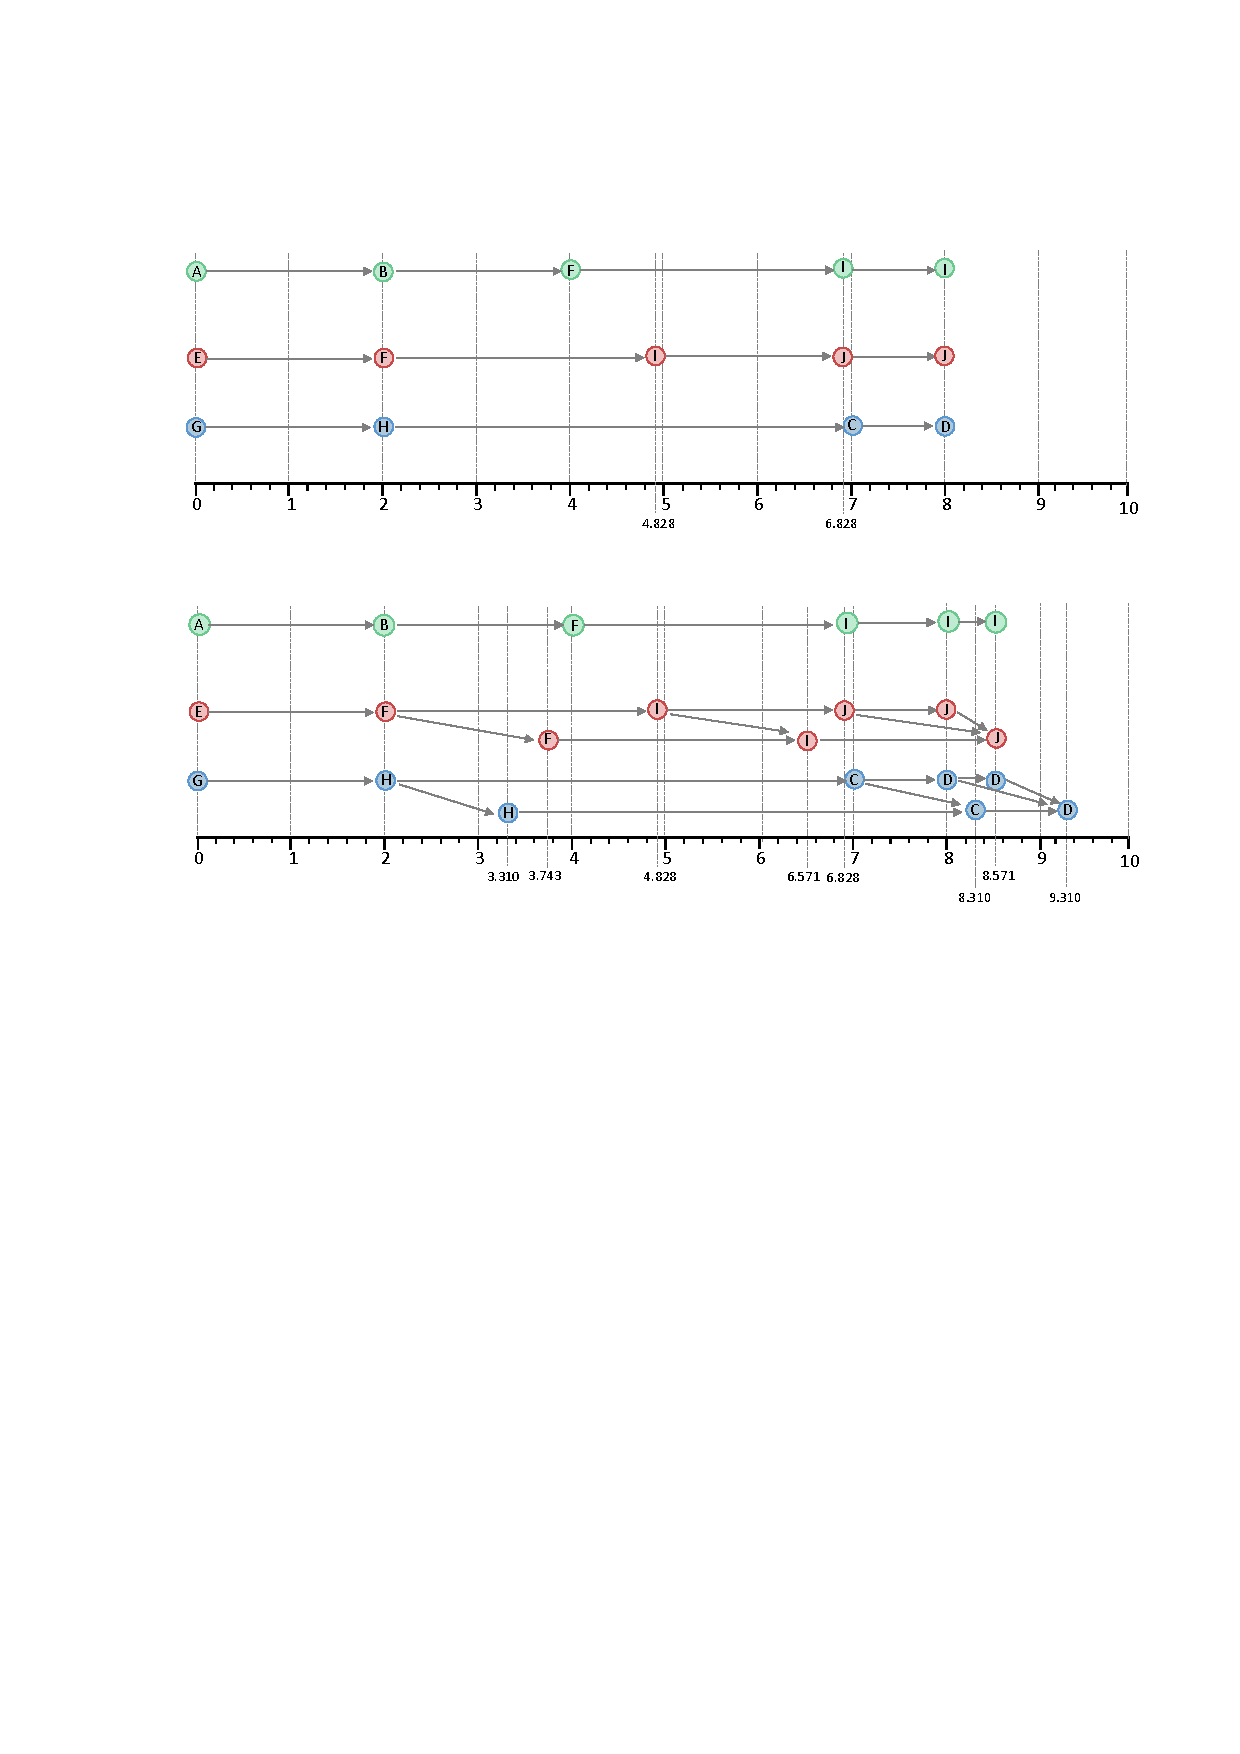
\includegraphics[trim={3.0cm 14.0cm 1.0cm 4.3cm},clip,width=\columnwidth]{fig-running_makespan.pdf}
	\caption{An illustration of \mddr s. 
		The upper part shows an initial \mddr for the \mapfr problem in Figure \ref{fig:example}. The lower part shows the \mddr for the same problem after resolving a conflict between the red and blue agents traversing $(F,I)$ and $(H,C)$ respectively.}
	\label{fig:mddr}
\end{figure}


\begin{example}
	Figure \ref{fig:mddr} shows the \mddrs for the agents in our running example (Figure~\ref{fig:example}). 
	The upper part shows the \mddrs created for each agent w.r.t. an empty set of constraints. 
	In our example, each agent has a single shortest single-agent plan, and so the \mddr 
	created for an empty set of constraints is a line. 
	The red and blue agents' plans have a conflict between the timed actions $(F\rightarrow I, 2.000)$ and $(H \rightarrow C, 2.000)$. 
	The unsafe intervals for these actions are $[2.000,3.310)$ and $[2.000,3.743)$, respectively. 
	So, the \ccbs constraints generated for this conflict are
	\begin{equation}
	\{ \tuple{red, (F\rightarrow I, 2.000), [2.000,3.310)}, 
	\tuple{blue, (H\rightarrow C, 2.000), [2.000,3.743)} \}
	\label{eq:example-constraints}
	\end{equation}
	The lower part of Figure~\ref{fig:mddr} shows the \mddr generated for each agent when considering the pair of \ccbs constraints in Equation (\ref{eq:example-constraints}).
\end{example}




\textbf{Step 3. Create a \ps.} We create in this step a \ps such that every satisfying assignment to it corresponds to a \mapfr solution in which each agent follows a single-agent plan from its \mddr. 
To create such a \ps, we create Boolean variables $\mathcal{E}_{v,v'}^{t,t'}(i)$ and $\mathcal{X}_{v}^{t}(i)$ 
for every edge and node in $E^i$ and $X^i$ respectively. 
Setting $\mathcal{X}_v^t(i)$ to true represents that agent $i$ plans to occupy location $v$ in time $t$. 
Setting $\mathcal{E}_{v,v'}^{t,t'}(i)$ to true represents that agent $i$ plans performs an action that start at time $t$, ends at time $t'$, and moves the agent from $v$ to $v'$. 
Note that wait actions are represented by $\mathcal{E}_{v,v'}^{t,t'}(i)$ variables with $v=v'$. 
To ensure that an assignment to all these variables constitutes a solution to the given \mapfr problem, 
we add the following restrictions over these Boolean variables to the \ps. %\konstantin{May be remove/substitute the word 'constraints' in this sentence and in the below paragraph (to avoid confusion with \ccbs constraints).}\roni{Changed to ``restrictions''. Not sure if this works.} 
\begin{equation}
{  \mathcal{X}_v^t(i) \Rightarrow \bigvee_{(v',t')\;|\;[(v,t);(v',t')] \in E^i}{\mathcal{E}^{t,t'}_{v,v'}(i)},
}
\label{eq-1}
\end{equation}

\begin{equation}
{  \sum_{(v',t')\:|\:[(v,t);(v',t')] \in E^i }{\mathcal{E}_{v,v'}^{t,t'}{(i)} \leq 1}
}
\label{eq-2}
\end{equation}
\begin{equation}
{  \mathcal{E}_{v,v'}^{t,t'}(i) \Rightarrow \mathcal{X}_{v'}^{t'}(i)
}
\label{eq-3}
\end{equation}
Equations~\ref{eq-1} and~\ref{eq-2} state that if agent $i$ appears in vertex $v$ at time $t$ then it has to leave through exactly one edge connected to $v$. 
Equation~\ref{eq-3} establishes that once an agent enters an edge in the \mddr it has to leave it at its endpoint. 
We also add to the \ps clauses that verify every agent starts in its start location and ends in its goal.
Thus, a satisfying assignment to this formula represents a solution to the given \mapfr problem. 


\textbf{Step 4. Add constraints to verify all conflicts are avoided.}
To avoid all the \ccbs conflicts in $\Psi$, we verify that for every conflict $Con\in\Psi$ one of the \ccbs constraints in $\const(Con)$ is satisfied. 
This is done by adding to the \ps created in step 3 
an appropriate disjunction. 
That is, for a conflict $\tuple{(a_i,t_i), (a_j, t_j)}$, where $a_i$ is the action that moves the agent $i$ from $v$ to $v'$ and $a_j$ -- moves agent $j$ from $u$ to $u'$, 
we add following clause:
\begin{equation}
	\neg \mathcal{E}^{t_i, t_i+{a_i}_D}_{v,v'}(i)
\vee
	\neg \mathcal{E}^{t_j, t_j+{a_j}_D}_{u,u'}(j)
\label{eq-mutex}
\end{equation}

\konstantin{Hmm. It seems to me now that having '$t_i, t_i+{a_i}_D$' in the superscript is not right. We should prohibit an agent to perform an action for a time interval that equals the imposed interval-constraint (not necessarily the duration of an action).}
\roni{Good question. After some thought, I think that it is correct as is. The reason is that the Boolean variables $\mathcal{E}^{t_i, t_i+{a_i}_D}_{v,v'}$ are created by analyzing the \mddr. So, we will not have any other superscript that is not of the form $(t, t+a_D)$. Only in the \mddr generation part do we enjoy the fact that the constraints forbid the timed action for an entire time range.}
\pavel{I was also tempted to use conflict interval only. But MDDr records actions with their original durations and this is only what forbid by this mutex constraint. In other words, we forbid pair of actions that led to the conflict.}

This clause represents mutual exclusion between the two conflicting actions. 
Thus having this clause in the \ps ensures at most one of these timed actions will be applied in any satisfying solution. 
%they will not be appliedcannot be executed together.  The resulting propositional formula is used in our algorithm as the \ps.

%PS Example
\begin{example}
Consider again our running example from Figure~\ref{fig:example}, 
and the three \mddr shown in the upper part of Figure~\ref{fig:mddr}. 
The variables created for the corresponding \ps , are:
\begin{multline*}
\mathcal{X}_B^{0.000}(1), \mathcal{X}_B^{2.000}(1), \mathcal{X}_F^{4.000}(1), \mathcal{X}_I^{6.828}(1), \mathcal{X}_I^{8.000}(1), \\
\mathcal{E}_{A,B}^{0.000,2.000}(1), \mathcal{E}_{B,F}^{2.000,4.000}(1), \mathcal{E}_{F,I}^{4.000,6.828}(1), \mathcal{E}_{I,I}^{6.828,8.000}(1)    
\end{multline*}
for agent 1 (green)
\begin{multline*}
    \mathcal{X}_E^{0.000}(2), \mathcal{X}_F^{2.000}(2), \mathcal{X}_I^{4.828}(2), \mathcal{X}_J^{6.828}(2), \mathcal{X}_J^{8.000}(2)\\
\mathcal{E}_{E,F}^{0.000,2.000}(2), \mathcal{E}_{F,I}^{2.000,4.828}(2), \mathcal{E}_{I,J}^{4.828,6.828}(2), \mathcal{E}_{J,J}^{6.828,8.000}(2)
\end{multline*}    
for agent 2 (red), and 
\begin{multline*}
    \mathcal{X}_G^{0.000}(3), \mathcal{X}_H^{2.000}(3), \mathcal{X}_C^{7.000}(3), \mathcal{X}_D^{8.000}(3) \\
\mathcal{E}_{G,H}^{0.000,2.000}(3), \mathcal{E}_{H,C}^{2.000,7.000}(3), \mathcal{E}_{C,D}^{7.000,8.000}(3)
\end{multline*}
for agent 3 (blue). 
%\konstantin{the last edge variable for the agent 3 is not needed, I believe. I meant that one: $\mathcal{E}_{J,J}^{6.828,8.000}(2)$.}\roni{I think it is needed to verify collisions at the goal node. What do you think?} \pavel{Final wait edges are needed since otherwise the agent could disappear for other agents. Like Roni said, collisions at the goal could not be detected if the edge is not there.}\konstantin{Guys, I'm saying about the last variable for the 3rd agent -- look at it -- it's about agent 2. I think it's just a 'copy-paste' error and should be removed :)} \pavel{3rd agent last variable deleted, C->D is the last action for it}.
These variables are used in the constraints defined by Equations~\ref{eq-1}-\ref{eq-mutex}. 
%Constraints defined by Equation \ref{eq-1} for agent 1 (green):\\
%$\mathcal{X}_A^{0.000}(1) \Rightarrow \mathcal{E}_{A,B}^{0.000,2.000}(1)$ \\ $\mathcal{X}_B^{2.000}(1) \Rightarrow \mathcal{E}_{B,F}^{2.000,4.000}(1)$ \\ $\mathcal{X}_F^{4.000}(1) \Rightarrow \mathcal{E}_{F,I}^{4.000,6.828}(1)$ \\ $\mathcal{X}_I^{6.828}(1) \Rightarrow \mathcal{E}_{I,I}^{6.828,6.828}(1)$ \\ The set of constraints defined by Equation \ref{eq-2} is empty and finally constraints defined by Equation \ref{eq-3} are as follows for agent 1 (green): $\mathcal{E}_{A,B}^{0.000,2.000}(1)$ \Rightarrow \mathcal{X}_B^{2.000}(1)$\\ $\mathcal{E}_{B,F}^{2.000,4.000}(1)$ \Rightarrow \mathcal{X}_F^{4.000}(1)$\\$\mathcal{E}_{F,I}^{4.000,6.828}(1)$ \Rightarrow \mathcal{X}_I^{6.828}(1)$\\ $\mathcal{E}_{I,I}^{6.828,6.828}(1)$ \Rightarrow \mathcal{X}_I^{8.000}(1)$\\
%Similar sets of constraints are introduced for agents 2 (red) and 3 (blue). 
In addition, we establish that each agent starts and ends in its start and goal location by setting the variables $\mathcal{X}_B^{0.000}(1)$, $\mathcal{X}_E^{0.000}(2)$, $\mathcal{X}_G^{0.000}(3)$ (start positions) and $\mathcal{X}_I^{8.000}(1)$, $\mathcal{X}_J^{8.000}(2)$, $\mathcal{X}_D^{8.000}(3)$ (goal positions) to \true.
The resulting formula can be solved easily by setting all variables to \true, which corresponds to the solution in which the agents do not wait in any position and go directly to their goals: agent 1 (green) goes from A to B to F to I, agent 2 (red) goes  from E to F to I to J, 
and agent 3 (blue) goes from G to H to C to D. 
% (line 3).What is this line? \pavel{refered to lines in Algorithm 3}\roni{But the algorithm is only introduced later.}
As noted earlier, this solution has a conflict, and the \mddr in the lower part of Figure~\ref{fig:mddr} is created by considering the \ccbs constraints designed to resolve this conflict. 
The \ps created for the three $MDD_R$s in the lower part of Figure~\ref{fig:mddr} includes additional variables representing new timed actions and locations the agent may now occupy. 
These variables are:
\begin{multline*}
\text{Agent 1 (green):} \mathcal{X}_I^{8.571}(1) \mathcal{E}_{I,I}^{8.000,8.571}(1)
\end{multline*}
\begin{multline*}
\text{Agent 2 (red):} \mathcal{X}_F^{3.743}(2), \mathcal{X}_I^{6.571}(2), \mathcal{X}_J^{8.571}(2), \mathcal{E}_{F,F}^{2.000,3.743}(2), \mathcal{E}_{F,I}^{3.743,6.571}(2),\\ \mathcal{E}_{I,J}^{6.571,8.571}(2)    
\end{multline*}
\begin{multline*}
    \text{Agent 3 (blue):}
    \mathcal{X}_H^{3.310}(3), \mathcal{X}_C^{8.310}(3),
\mathcal{X}_D^{9.310}(3), 
\mathcal{E}_{H,H}^{2.000,3.310}(3), \mathcal{E}_{H,C}^{3.310,8.310}(3),\\ \mathcal{E}_{C,D}^{8.310,9.310}(3)
\end{multline*}
Additional clauses are added for these variables following Equations~\ref{eq-1}--\ref{eq-3}. 
In addition, the following clause it added as specified in Equation~\ref{eq-mutex}
\begin{equation}
  \neg \mathcal{E}_{F,I}^{2.000,4.828}(2) \vee \neg \mathcal{E}_{H,C}^{2.000,7.000}(3).
\end{equation}
to verify that the conflict identified in the previous solution will be avoided.
\end{example}

\begin{theorem}
	\musmtccbs is a sound and complete algorithm for bounded-cost \mapfr, 
	i.e., every solution returned by \musmtccbs is indeed a solution with makespan equal to or smaller than the makespan bound, 
	and if such a solution exists then it will be found. 
	\label{the:bounded-cost-makespan}
\end{theorem}
Soundness is established by the fact that \decidemapfr verifies that the returned solution is valid. Establishing completeness, however, is less trivial. A formal proof is given in~\ref{app:completeness}. 


\subsection{\smtccbs}
\label{sec:musmtcbs}
\begin{algorithm}[h]
	\SetKwInOut{Input}{Input}
	\Input{$P$, the \mapfr problem}
	
	%$\Psi \gets \emptyset$\\
	$\Pi \gets \{\pi_1,\ldots,\pi_k \}$, where $\pi_i$ is the shortest single-agent plan for agent $a_i$ \\
	$\mu \gets \max_{i=1}^k{\mu(\pi_i)}$ \\
	\While {True}{
		$\Pi \gets$ $\mu$\smtccbs($P$, $\mu$)\\
		\If {$\Pi$ is not null}{
			\Return $\Pi$\\
		}
		$\mu \gets $ Compute next $\mu$ \nllabel{line:smtccbs:nextmu}\\
	}
	\caption{Pseudo code for \smtccbs} \label{alg-SMTCBS-high}
\end{algorithm}
Finally, we can present our \smtccbs algorithm. Pseudo code is listed in Algorithm~\ref{alg-SMTCBS-high}. 
It starts by setting the makespan-bound $\mu$ to the single-agent plan with the longest duration. Then, it runs $\mu$\smtccbs to try to find a valid solution whose makespan is $\mu$. If it succeeded, it returns that solution. Otherwise, $\mu$ is increased to the next relevant makespan (line~\ref{line:smtccbs:nextmu}). 
The next relevant makespan is set by adding to $\mu$ the minimal amount that enables at least one more action by at least one agent. In our implementation we computed the next relevant makespan while $\mu\smtccbs$ computes the \mddr for each agent. 
This was done by keeping track of the minimum of end times of move actions $a \in A$ that starts before the makespan bound but ends after. 


\begin{theorem}
\smtccbs is sound, complete, and is guaranteed to return a makespan-optimal solution. 
\label{the:optimal-makespan}
\end{theorem}
\begin{proof}
Every solution returned by \smtccbs is also a solution to \
Soundness and completeness follows from the soundness and completeness of \musmtccbs, established in Theorem~\ref{the:bounded-cost-makespan}.

\musmtccbs returns a solution then it is a valid solution of given \mapfr problem $P$ satisfying given makespan $\mu$. This claim relies on the soundness of encoding where possible satisfying assignments of the formula correspond to paths of length at most $\mu$ connecting starting and goal positions of agents. In addition to this \decidemapfr verifies that individual paths are non-conflicting.
The iterative scheme for trying larger makespans follows the idea from \mddsat~\cite{DBLP:conf/ecai/SurynekFSB16}. To find an optimal makespan we need to ensure that the iterative process does not skip any relevant makespan. Having a set of constraints $\const(\Psi)$ in the course of the \smtccbs algorithm including sound pairs of constraints (Definition \ref{def:sound}) then any solution to given \mapfr problem $P$ must satisfy this set of constraints. After the compete failure for given makespan $\mu$ in $\mu$\smtccbs we know due to the completeness of \musmtccbs that there is no solution of makespan $\mu$. Then we proceed to the next makespan $\mu_{next}$ which is set according to current set of constraints $\const(\Psi)$.
The sufficient condition to have the makespan increasing scheme sound and optimal is that we should have a chance to obtain a new feasible solution w.r.t. $\const(\Psi)$ at the next $\mu_{next}$ while for makespans between $\mu$ and $\mu_{next}$ no feasible solution w.r.t. $\const(\Psi)$ should exist to ensure that we do not skip any relevant makespan. This is done by computing all-single agents plans CSIPP would generate for $\const(\Psi)$ but we allow it going beyond the makespan bound $\mu$ by making one extra action. The smallest action finish time beyond $\mu$ over all such plans is taken as the next makespan bound $\mu_{next}$. Existence of a solution satisfying $\const(\Psi)$ of makespan $\mu'$ such that $\mu' > \mu \wedge \mu' < \mu_{next}$ would contradict the definition of $\mu_{next}$. Hence no such solution exists and the makespan increasing scheme guarantees finding optimal solution. %Existence of a solution of makespan $\mu'$ such that $\mu' > \mu \wedge \mu' < \mu_{next}$ would contradict the fact that $Cons(\Psi)$ must be satisfied by any solution.
\pavel{Suggesting separate paragraph here. Content seems okay.} Note that \smtccbs, like \ccbs, is \emph{solution complete}~\cite{walker2020bipartite}. 
%complete in a weak way. \konstantin{I saw in a recent paper that this might be attributed as being 'solution complete'. May be we also adopt it, i.e. substitute 'weak way' for 'solution complete'?}\roni{I like this a lot. Do you mean this paper:https://goldberg.berkeley.edu/pubs/completeness.pdfFrom a quick read, it seems that they use ``solution complete'' as a property of a problem, to say that it always has a solution. Did you see it used in the context of algorithms?}\konstantin{That's the paper I was talking about: https://www.aaai.org/Papers/AAAI/2020GB/AAAI-WalkerT.2901.pdf. They explicitly attribute CBS as being solution complete (see p.2 on the left).}\roni{This is perfect, it is also from our domain. Changing the text above accordingly}
That is, if a valid solution exists, \smtccbs will find it. Unsolvability cannot be detected by \smtccbs.
\end{proof}


\section{Experimental Evaluation}
\label{sec:experiments}

\begin{figure*}[t]
\centering
\begin{subfigure}
    \centering
    \begin{subfigure}
        \centering
        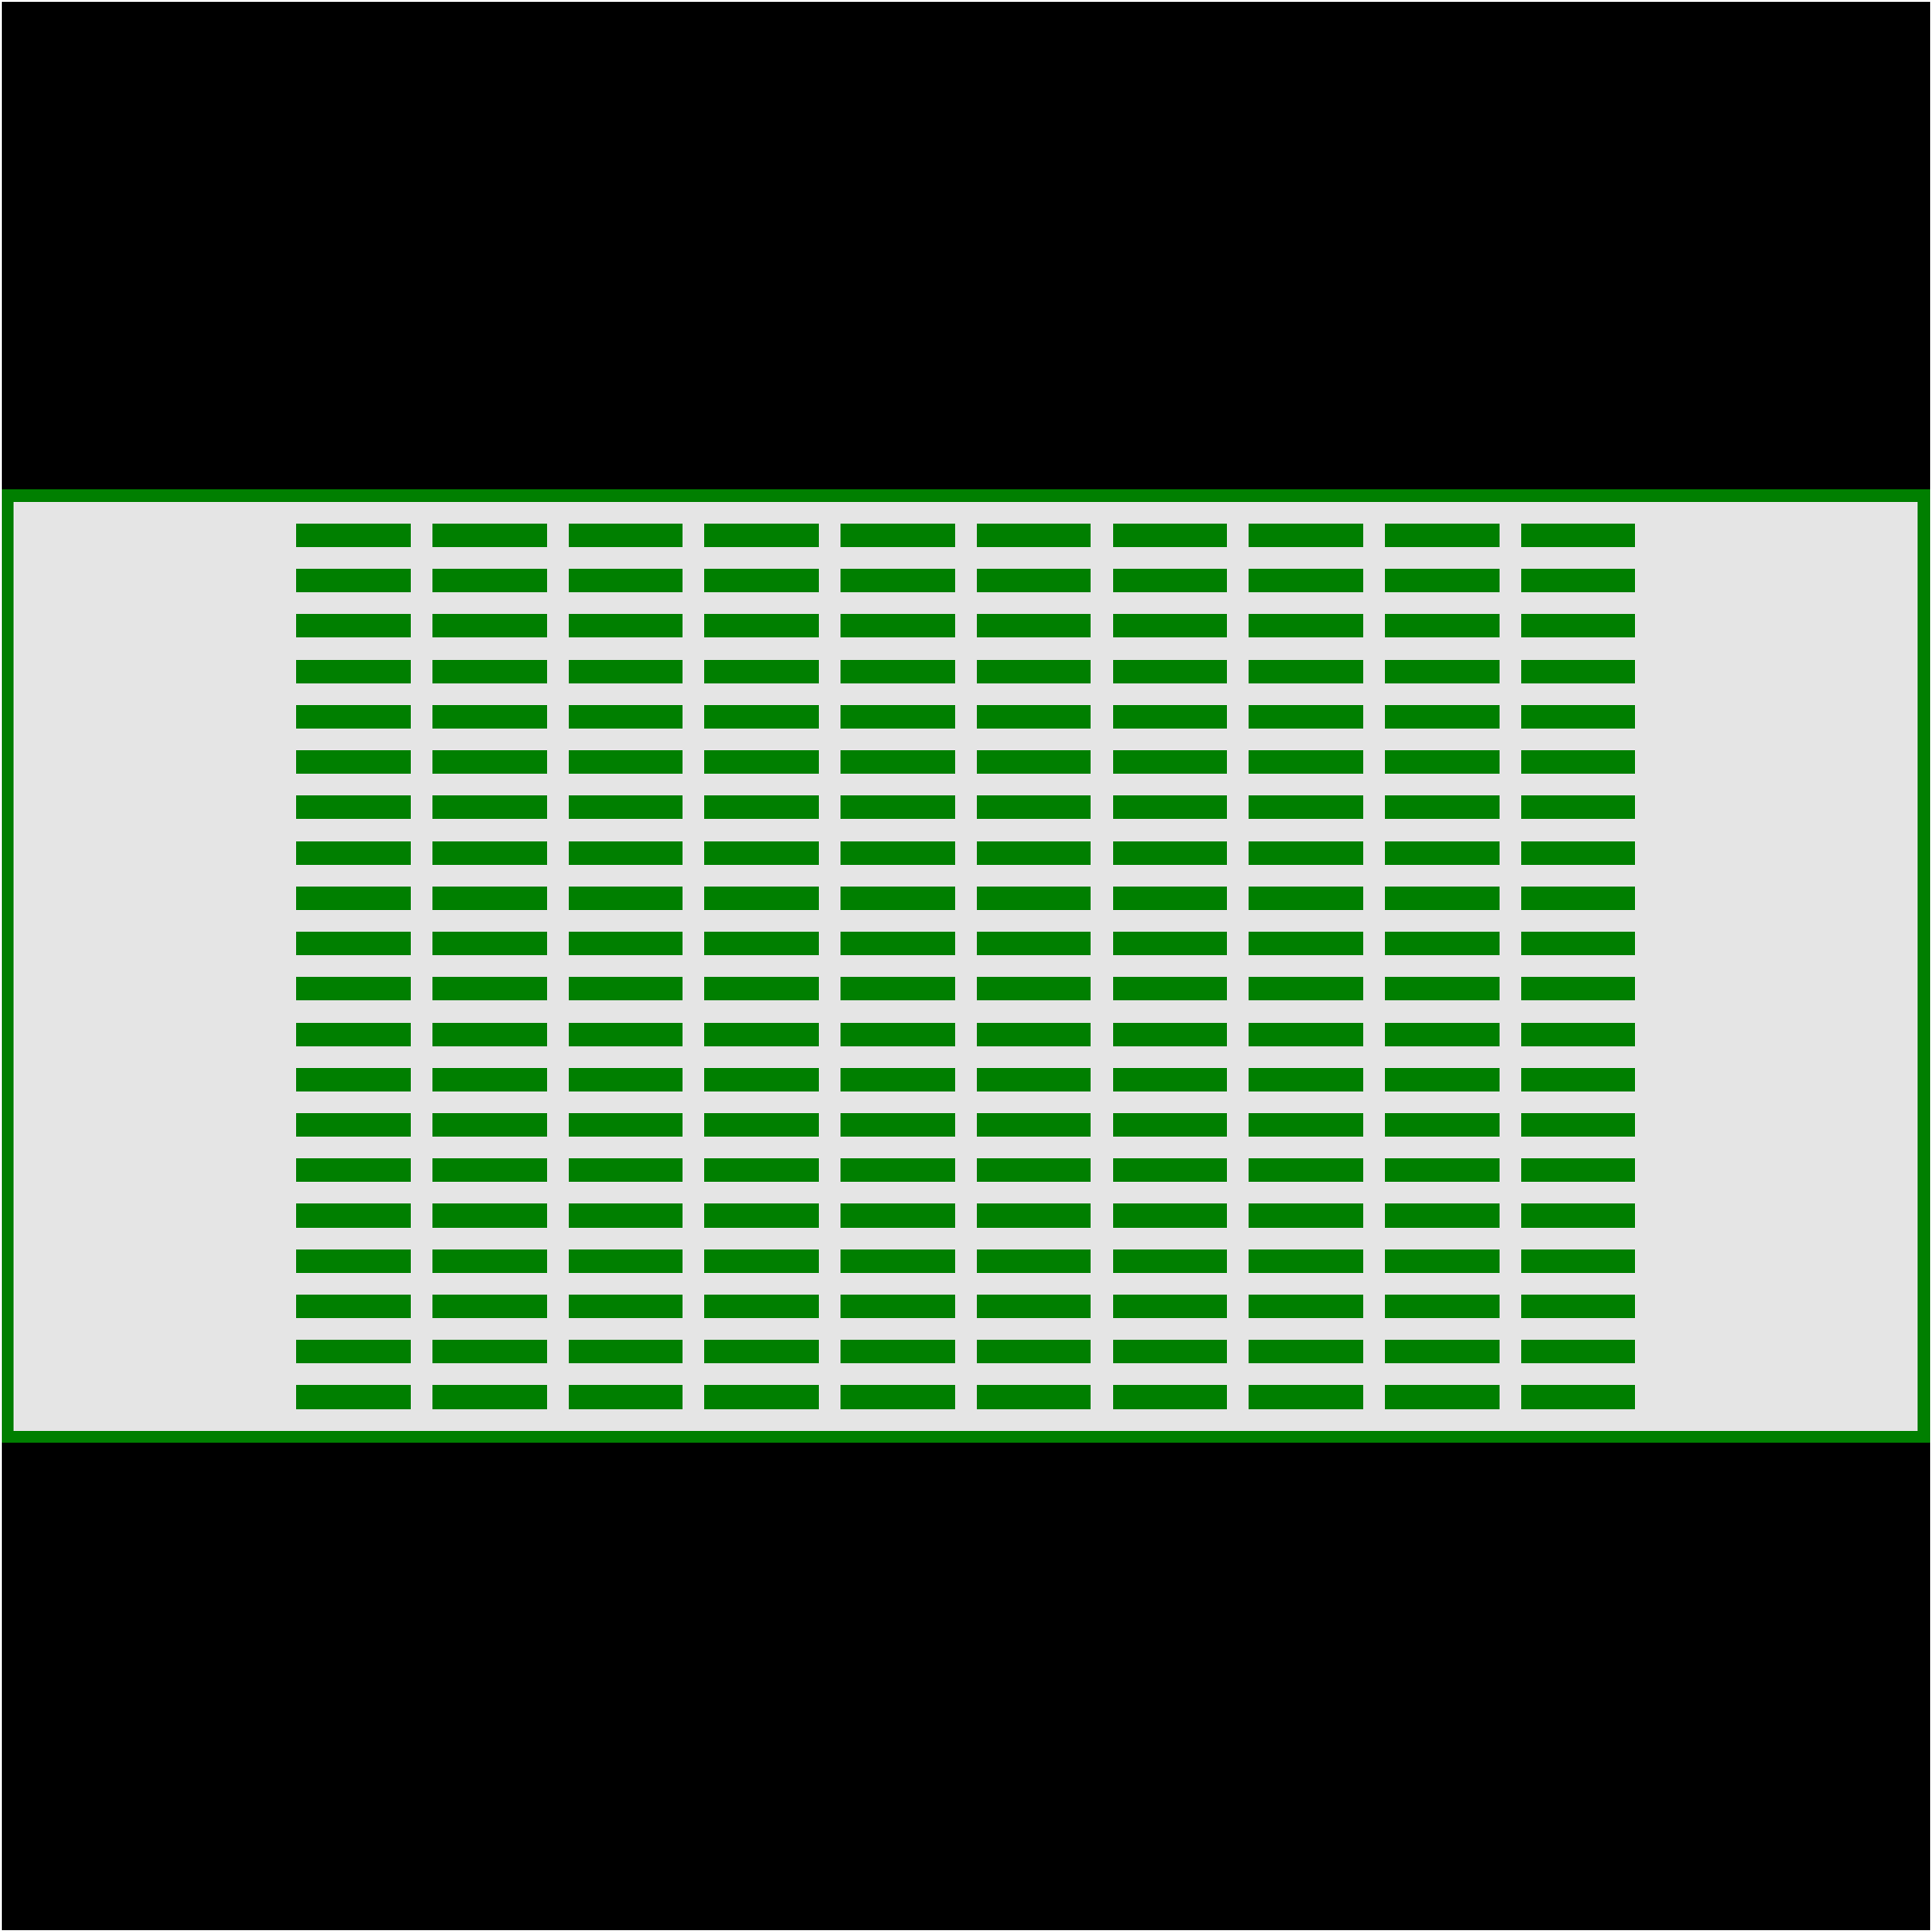
\includegraphics[width=0.3\linewidth]{gridmap-warehouse-10-20-10-2-2.pdf}
        %\caption{}
        %\label{}
    \end{subfigure}\hspace{0.025\linewidth}%
    \begin{subfigure}
        \centering
        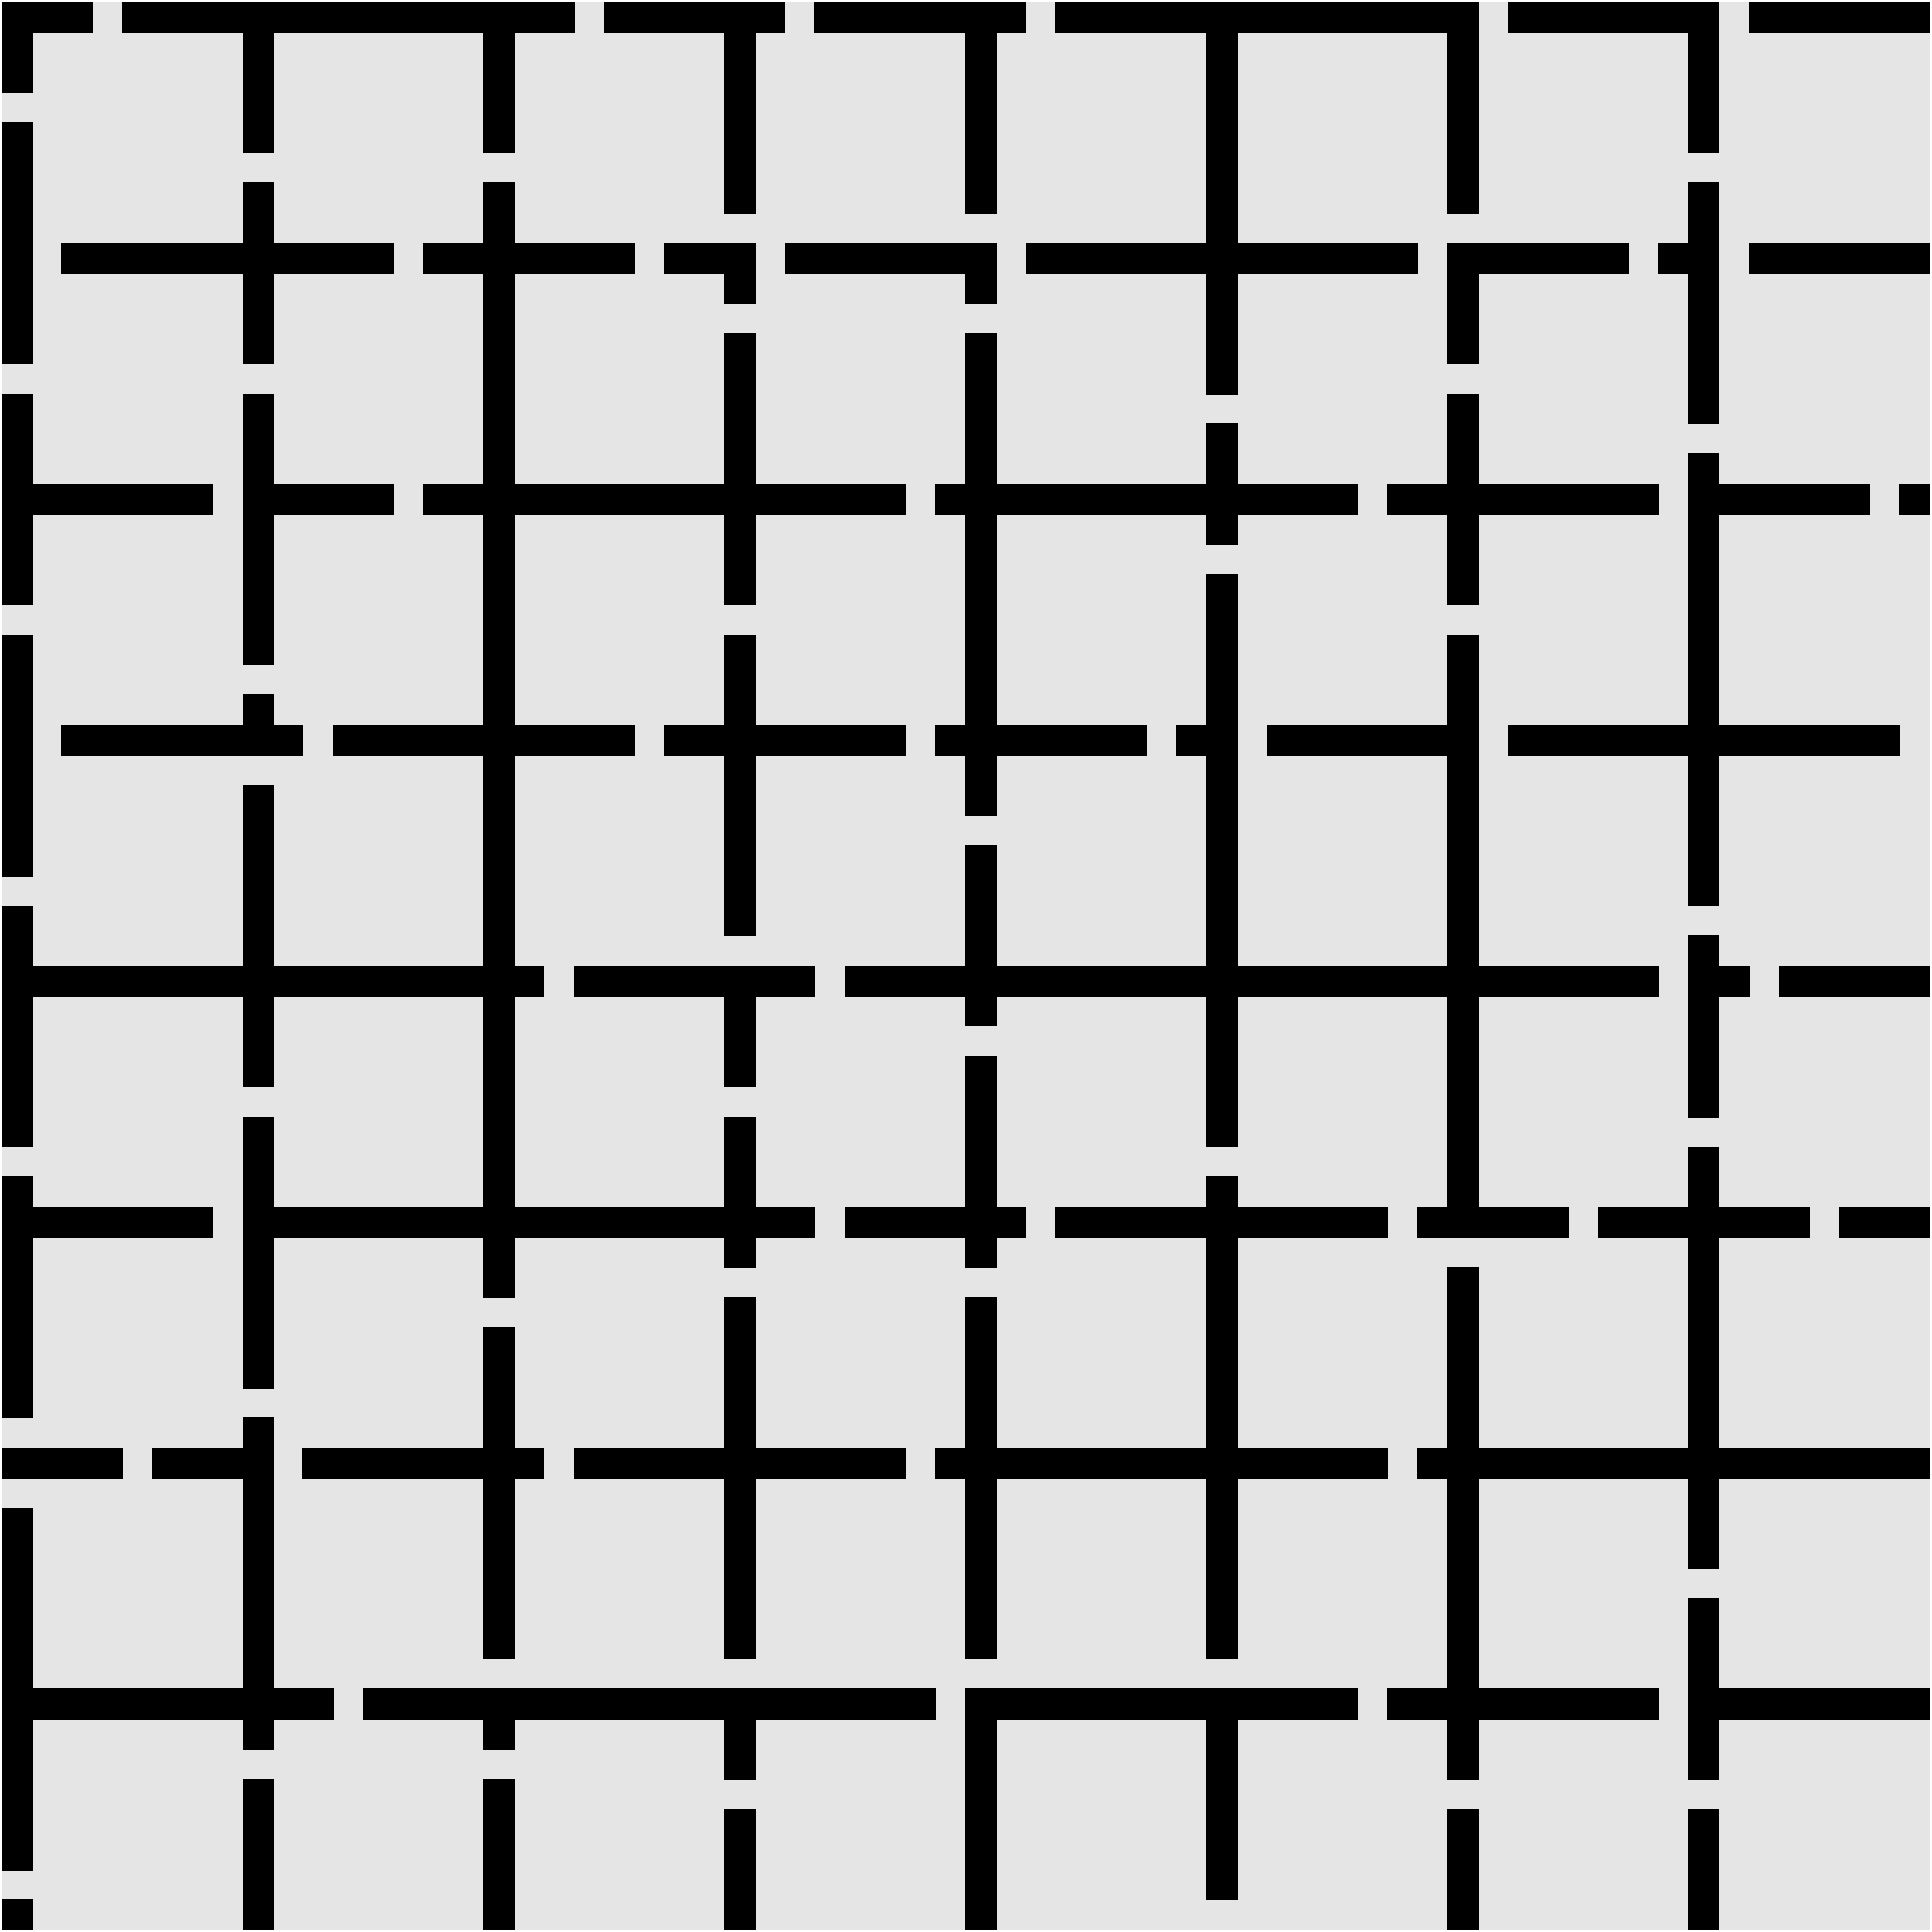
\includegraphics[width=0.3\linewidth]{gridmap-room-64-64-8.pdf}
        %\caption{}
        %\label{}
    \end{subfigure}\hspace{0.025\linewidth}%
    \begin{subfigure}
        \centering
        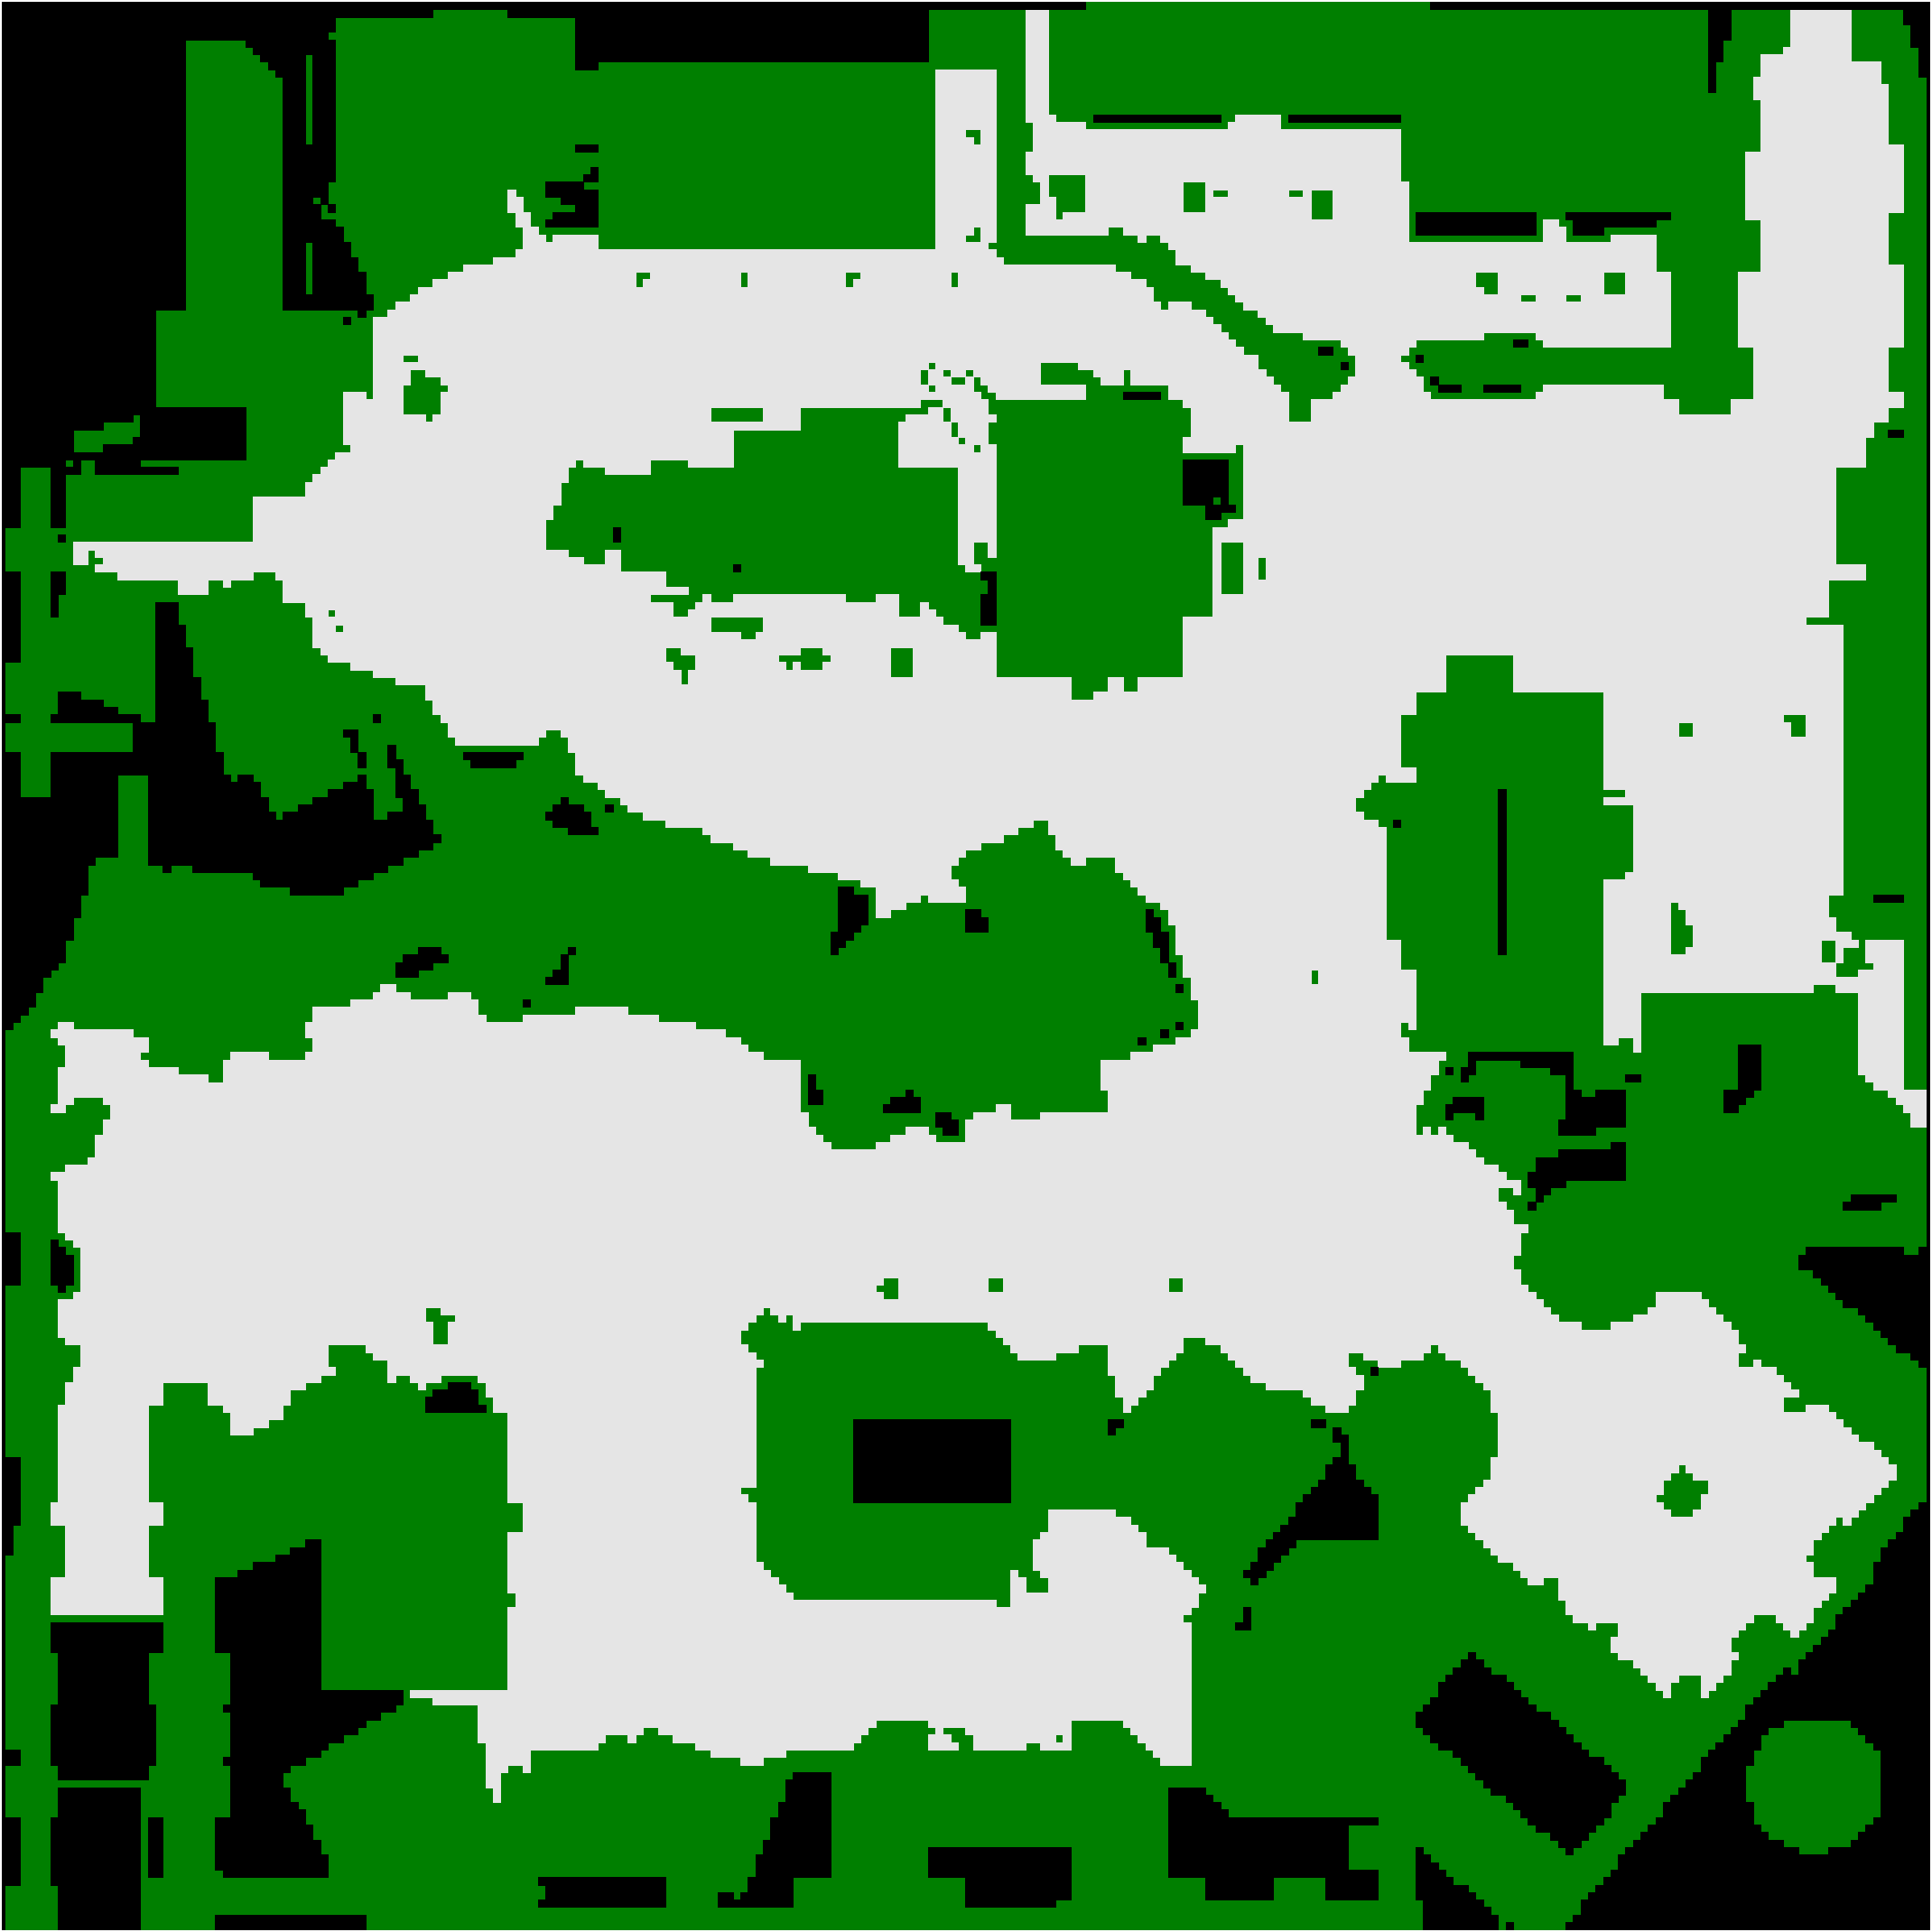
\includegraphics[width=0.3\linewidth]{gridmap-den520d.pdf}
        %\caption{}
        %\label{}
    \end{subfigure}%\hspace{0.025\linewidth}%
\end{subfigure}
\caption{Maps used for the evaluation of \ccbs and \smtccbs. From left to right: \texttt{warehouse-10-20-10-2-2}, \texttt{room-64-64-8}, \texttt{den520d}.}
\label{fig:gridmaps}
\end{figure*}

%\subsection{Setup} \roni{It is not nice to start a section with a subsection.}
We implemented \ccbs and \smtccbs, and evaluated their performance on a range of \mapfr problems.
In this section, we report the results of this evaluation. 

\subsection{Experimental Setup}
In our experiments, we used two types of graphs: $2^k$-neighborhood grids \cite{rivera2017grid} and graphs that represent roadmaps.


% Grids
\subsubsection{$2^k$-Neighborhood Grids} 
For the 
$2^k$-neighborhood grid graphs, we used the grids
\texttt{empty-16-16} ($16 \times 16$), \texttt{warehouse-10-20-10-2-2} ($161 \times 63$), \texttt{room-64-64-8} ($64 \times 64$), and \texttt{den520d} ($256 \times 257$) 
from the recently introduced grid-based \mapf benchmark~\cite{stern2019mapf} in the Moving AI repository~\cite{sturtevant2012benchmarks}.\footnote{\url{https://movingai.com/benchmarks/mapf.html}} 
 Fig.~\ref{fig:gridmaps} provides a visual representations of these grids.
We chose these specific grids from the grid-based \mapf benchmark as they represent different settings in which \mapfr problems arise, including video-games (\texttt{den520d}), warehouse logistics (\texttt{warehouse-10-20-10-2-2}), indoor robotics (\texttt{room-64-64-8}), and field robotics (\texttt{empty-16-16}).




\begin{figure*}[t]
\centering
\begin{subfigure}
    \centering
    \begin{subfigure}
        \centering
        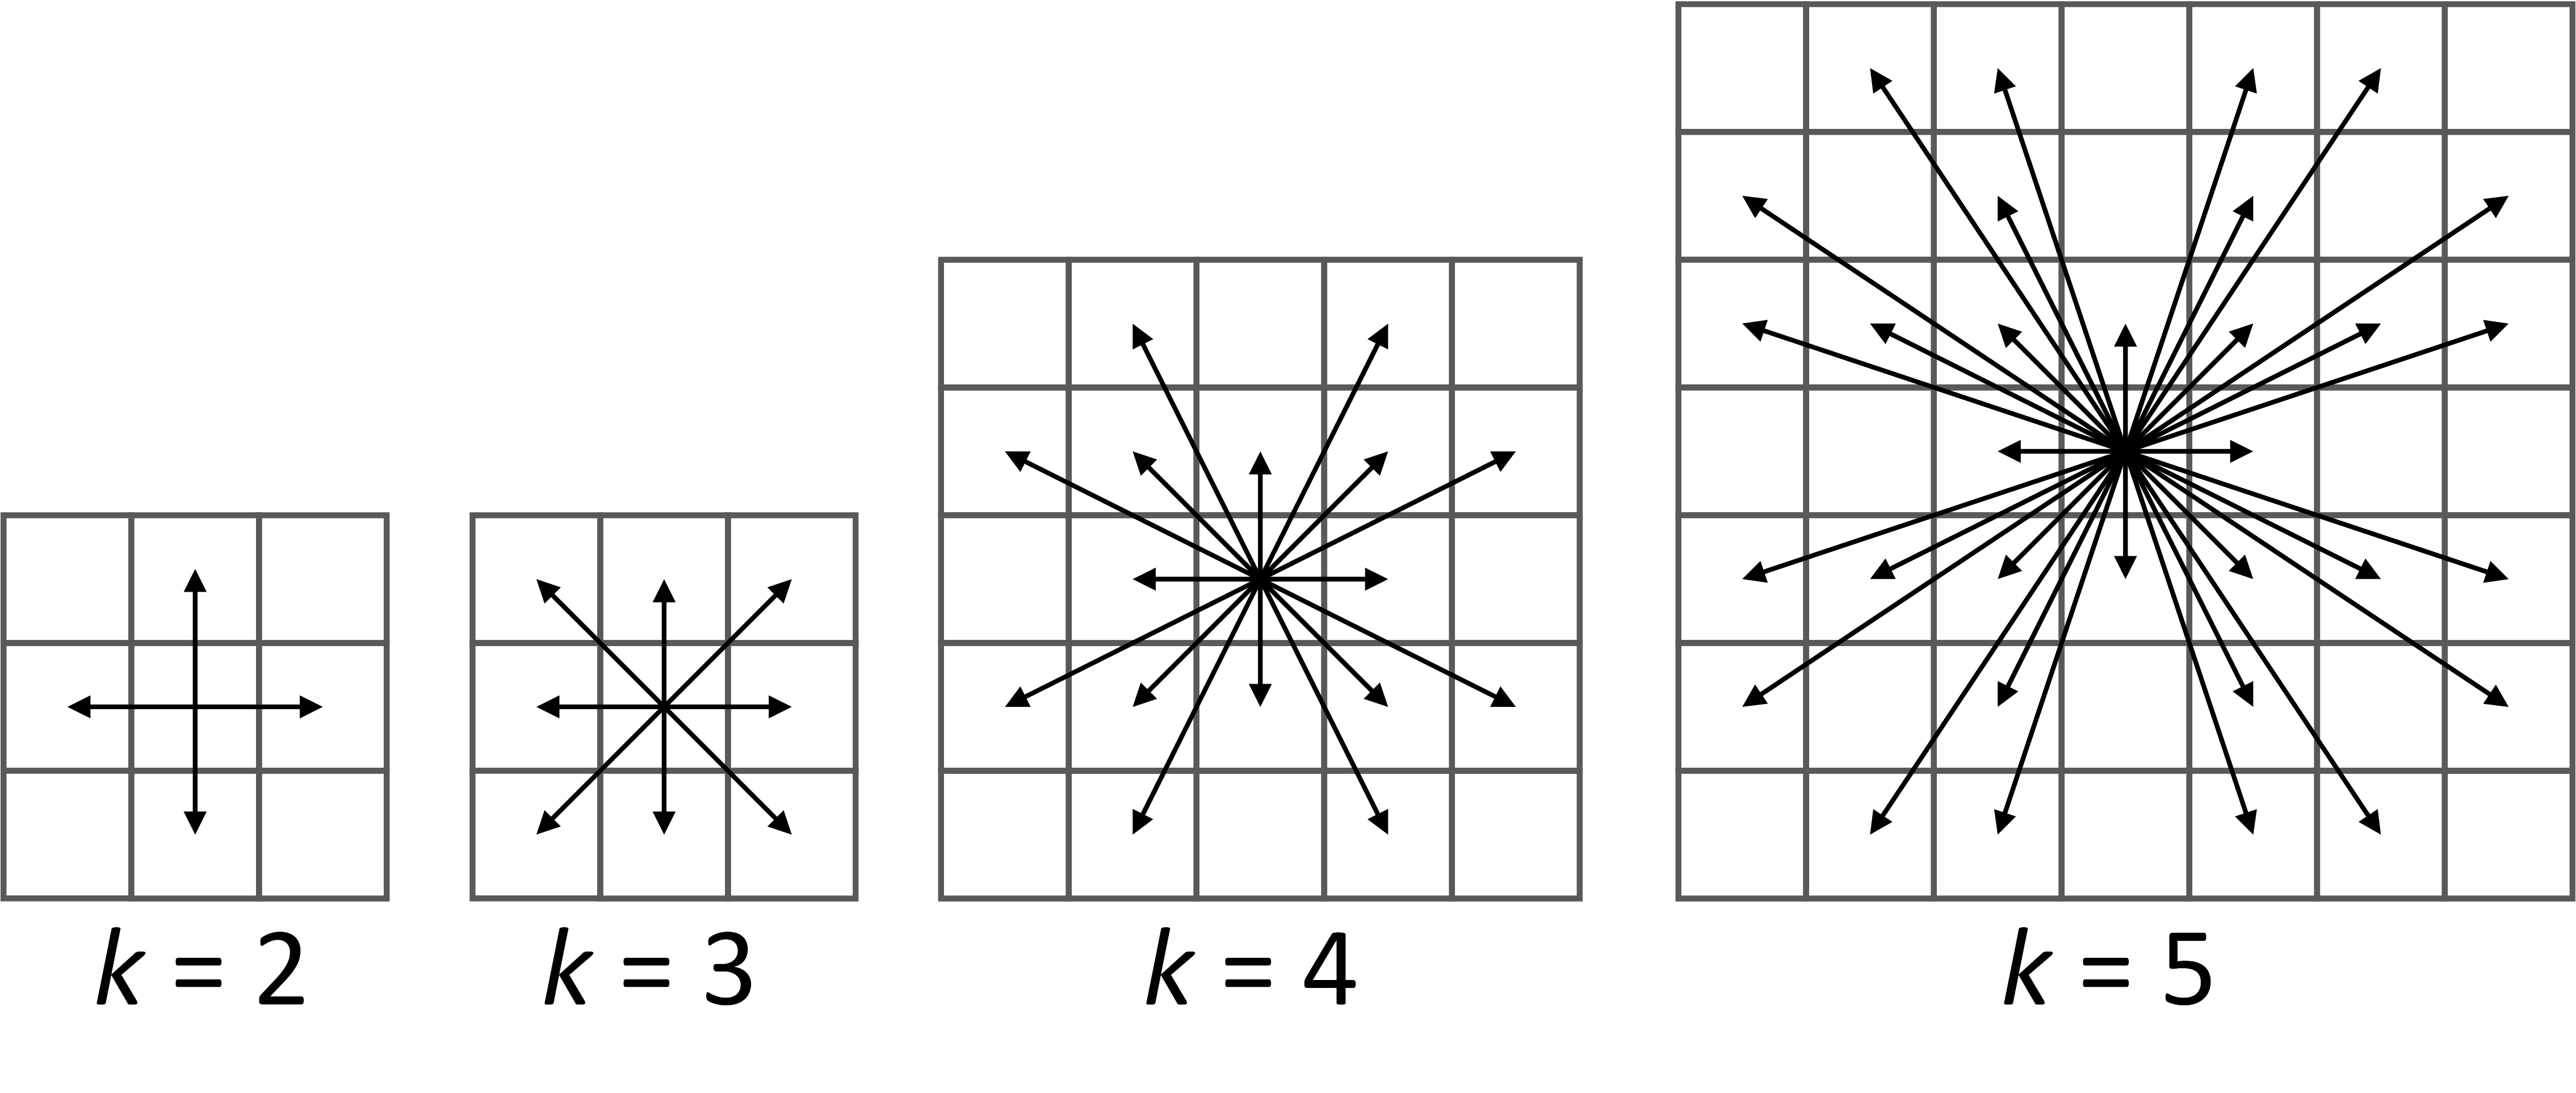
\includegraphics[width=0.7\linewidth]{2k-neighborhood.png}
        %\caption{}
        %\label{}
    \end{subfigure}\hspace{0.025\linewidth}%
    \begin{subfigure}
        \centering
        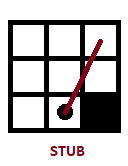
\includegraphics[width=0.25\linewidth]{MAPFr-invalid-move-on-a-grid.png}
        %\caption{}
        %\label{}
    \end{subfigure}%\hspace{0.025\linewidth}%
\end{subfigure}

\caption{(\emph{Left}) Illustration of the $2^k$ neighborhood for $k=2,3,4,$ and $5$. (\emph{Right}) An invalid move on a 16-connected grid. Although the source and target cells are unblocked and the line connecting them does not intersect the blocked cell, a disk-shaped agent of radius $\sqrt{2}/{4}$ will run into the latter in case the move is executed.}
\label{fig:2k-grids-and-invalid-move}
\end{figure*}

%\begin{figure}
%\centering
%    \centering
%    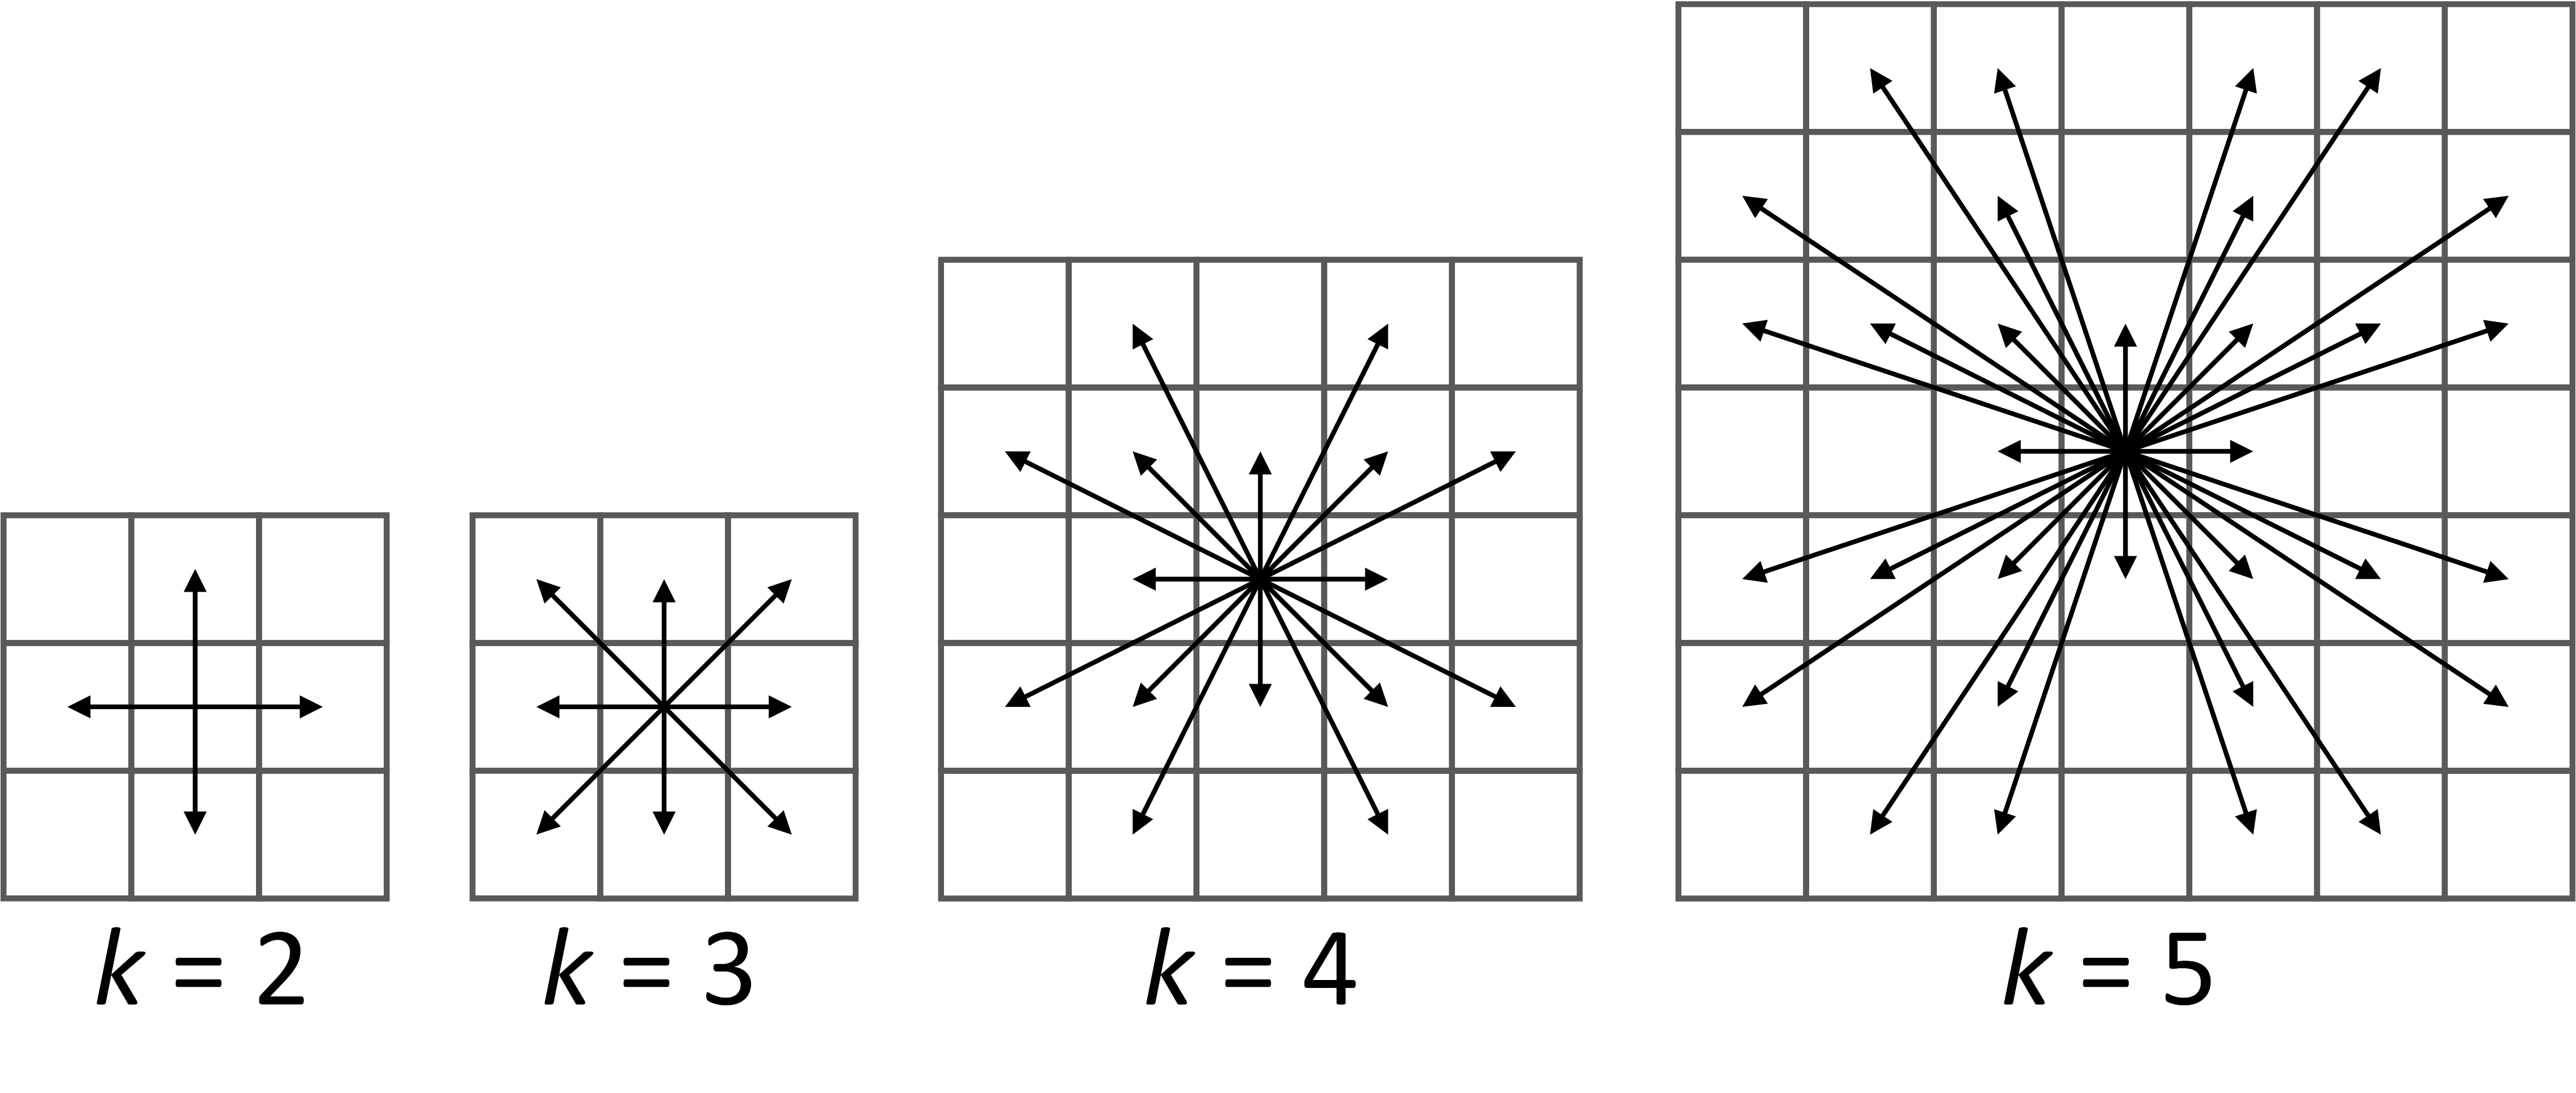
\includegraphics[width=0.75\linewidth]{2k-neighborhood.png}
%    \caption{Illustration of the $2^k$ neighborhood for $k=2,3,4,$ and $5$.}
%    \label{fig:2k-grids}
%\end{figure}

%\begin{figure}
%\centering
%    \centering
%    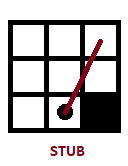
\includegraphics[width=0.25\linewidth]{MAPFr-invalid-move-on-a-grid.png}
%    \caption{An example of the invalid move on a 16-connected grid. Although the source and the target cells are unblocked and the line connecting the centers of those cells does not intersect the blocked cell, a disk-shaped agent of radius $\frac{\sqrt{2}}{4}$ will run into the latter in case the move is executed.}
%    \label{fig:MAPFr-invalid-move-on-a-grid}
%\end{figure}


%\begin{figure}
%\centering
%    \centering
%    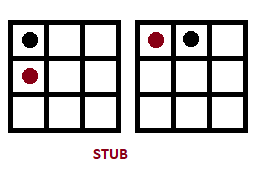
\includegraphics[width=0.5\linewidth]{classical-MAPF-common-manoeuvre.png}
%    \caption{A common manoeuvre in classical \mapf. Initial configuration is shown on the left and both agents start moving at the same time. The resultant configuration is shown on the right. In \mapfr such a manoeuvre can be executed by the identical in size disk-shaped agents \emph{iff} their radius is less or equal to $\sqrt{2}/4$.}
%    \label{fig:classical-MAPF-common-manoeuvre}
%\end{figure}



For each grid, the connectivity was set to $2^k$ where $k$ varied from $2$ to $5$ (see Fig.\ref{fig:2k-grids-and-invalid-move}). We ignored inertial effects and assumed the moving speed of each agent to be one grid cell per one time unit. That is, in one time unit an agent covers the segment whose length is equal to the distance between two adjacent grid cells. 
This does not mean the duration of all move actions is unit. 
For example, the duration of a move action from grid cell (x,y) to (x+1,y+1) is $\sqrt{2}$. \pavel{Why coordinates are not in the math style?}
Agents' shapes were disks of radius $\sqrt{2}/{4}$. %This specific size was chosen as this is the maximal size when disk agents with volume can both simultaneously perform a manoeuvre, shown in Fig.~\ref{fig:classical-MAPF-common-manoeuvre}, that is somewhat common in classical \mapf. \konstantin{Not sure how to explain this in elegant way}.

The shape of an agent was considered when checking collisions with static obstacles as well as other agents. Thus, if the segment representing a move action starts and ends in empty grid cells but the disk that moves along this segment intersects any of the blocked cells, then this action is prohibited. See Fig.~\ref{fig:2k-grids-and-invalid-move}(right) for example.


This grid-based \mapf benchmark~\cite{stern2019mapf} also provides \emph{scenario} files for each grid. 
Each scenario file lists start and goal locations for the agents. We used this list to create \mapfr problems in the way suggested by the maintainers of the benchmark. We started with one agent on a map and sequentially added one agent at a time by taking the next start-goal pair from the scenario file, until an algorithm was not able to solve a problem in a given time limit, which we set to 30 seconds. 
In our experiments, we generated \mapfr problems in this way, using all the 25 \texttt{random} scenario files available for each grid. 
Overall, for each grid and specific number of agents we ran the evaluated algorithms on 25 different \mapfr problems.




\subsubsection{Roadmap Graphs}
The second type of graphs we used in our experiments represent \emph{roadmaps}. 
We generated three different types of graphs -- \texttt{sparse}, \texttt{dense}, and \texttt{mega-dense} -- by processing the \texttt{den520d} map with a roadmap-generation tool which is a part of the Open Motion Planning Library (OPML) \cite{sucan2012opml}. This tool is widely used in the robotics community. The resulting roadmap graphs differ in their sizes: \texttt{sparse} includes 169 vertices and 349 edges, \texttt{dense} -- 878 vertices and 7341 edges, and \texttt{mega-dense} -- 11,342 vertices and 263,533 edges. The roadmap graphs are depicted in Fig.~\ref{fig:roadmaps}. Please note, that the \texttt{mega-dense} roadmap graph contains so many edges that they visually overlap.

\mapfr problems for these roadmap graphs were generated in a similar way as described above for the grid-based graphs. First, we generated 25 scenarios that contain non-overlapping start-goal pairs chosen randomly out of the graph vertices.
%\roni{You generated them or used existing scenario files?} \konstantin{We generated scenario files for each roadmap on our own. Scenario files from the repository contains start-goal locations that are tied to the grid cells. We don't have cells in the roadmaps.} 
Then we again started with one agent on a graph and sequentially adding one agent at a time by taking the next start-goal pair from the scenario file until the algorithm was not able to solve a problem in a 30 seconds time limit.

All the scenario files used in our experiments are publicly available at: \url{https://tinyurl.com/ccbs-instances}.

\begin{figure*}[t]
\centering
\begin{subfigure}
    \centering
    \begin{subfigure}
        \centering
        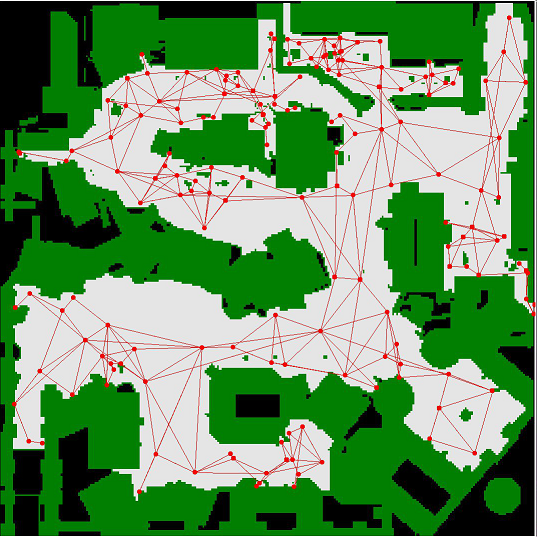
\includegraphics[width=0.3\linewidth]{den520d-roadmap-sparse.png}
        %\caption{}
        %\label{}
    \end{subfigure}\hspace{0.025\linewidth}%
    \begin{subfigure}
        \centering
        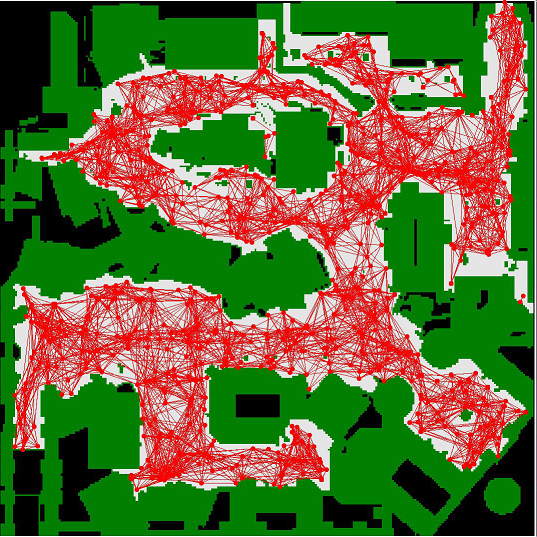
\includegraphics[width=0.3\linewidth]{den520d-roadmap-dense.png}
        %\caption{}
        %\label{}
    \end{subfigure}\hspace{0.025\linewidth}%
        \begin{subfigure}
        \centering
        \includegraphics[width=0.3\linewidth]{den520d-roadmap-mega-dense.png}
        %\caption{}
        %\label{}
    \end{subfigure}%\hspace{0.025\linewidth}%
\end{subfigure}

\caption{Roadmaps used in the experiments. Left -- \texttt{sparse}, center -- \texttt{dense}, right -- \texttt{mega-dense}.}
\label{fig:roadmaps}
\end{figure*}

\subsubsection{Design Choices and Implementation Details}

One of the major design choice one has to make when implementing an algorithm from the \cbs family is which conflict to choose when processing a high-level node. 
In classical \mapf, choosing conflicts in an intelligent can significantly reduce the number of the expanded \ct nodes and speed up the search by several orders of magnitude~\cite{boyarski2015icbs,boyrasky2015don}.
%Previous research on this topic in classical \mapf \cite{boyarski2015icbs,boyrasky2015don} 
%\konstantin{Guys, help me with the right links} 
%provides a clear evidence that choosing the conflicts in a smart way may significantly reduce the number of the explored \cbs nodes and speed up the search up to one order of magnitude or higher.
%\konstantin{Am i not exaggerating?}. Roni: No, this is true
%\konstantin{Roni, you've cut out mentioning classical MAPF here. I think it is needed as it is not 100\% evident that in MAPFr the same technique can always be applied. E.g. on roadmaps there is almost no symmetry and (almost) all conflicts are non-cardinal.}\roni{Fixed}
A particularly effective method for choosing conflicts is to prefer \emph{cardinal} conflicts over \emph{semi-cardinal} conflicts, and \emph{semi-cardinal} conflicts over \emph{non-cardinal} conflicts. 
A \cbs conflict is called cardinal \emph{iff} resolving it using either of corresponding \cbs constraints results in increasing the solution cost. 
The conflict is semi-cardinal if the solution cost increases only when imposing the corresponding \ccbs constraint on only one of the agents involved in the conflict. In all other cases the conflict is non-cardinal.

Effectively implementing this prioritization of cardinal and non-cardinal conflicts in \ccbs is not trivial, since conflict detection in \mapfr is much more costly than in classical \mapf. 
In our \ccbs implementation, we store all detected conflicts with their types (cardinal, semi-cardinal, or non-cardinal) in the nodes of the \ccbs constraint tree. 
When a child \ct node is generated, it immediately copies all the conflicts from its parent, except those that were resolved. Then, we detect conflicts only with the newly constructed plan, and identify their type (cardinal, semi-cardinal, or non-cardinal). This allowed choosing cardinal and semi-cardinal conflicts first in an effective manner, which in turn proved to be very effective for speeding up \ccbs. 
Note that in a preliminary version of this work~\cite{andreychuk2019multi}, we proposed a heuristic for choosing when to detect cardinal conflicts and when to avoid doing so. This heuristic does not yield significant improvement when using the described-above implementation for detecting conflict types. 

%(all other conflicts are copied from the parent node). \konstantin{Not sure that this paragraph is 100\% needed. What do you think?}

%Preferring cardinal conflicts to semi-cardinal to non-cardinal showed to work well for \mapfr as well. However, in \ccbs the computational cost of identifying to which class a \ccbs conflict belongs is, presumably, higher than for \cbs as now ... \konstantin{TODO: add the arguments why it is true or reformulate the sentence}. In our previous work \cite{andreychuk2019multi} we tried to avoid these computations in cases that seem no-promising and introduced a special heuristic for that. Nevertheless, after conducting more thorough evaluation we came to a conclusion that such a strategy does not lead to a desired result (lowering down the number nodes explored at the high level) in a range of cases. Thus, in this work we always detected whether the newly encountered conflicts are cardinal, semi-cardinal or non-cardinal and prefer the former to the latter. Among the conflicts of the same cardinality-type we chose to process the one that occurs earlier in time.

%Implementation wise we store all the conflicts (with their types) in the nodes of \ccbs constraint tree (CT). Thus, when a child CT node is generated we have to identify the cardinality-type only for the conflicts that are caused by a newly constructed plan for a constrained agent (all other conflicts are copied from the parent node). \konstantin{Not sure that this paragraph is 100\% needed. What do you think?}\roni{Will to 31.3.20}

An additional \ccbs design choice that is worth mentioning is the tie-breaking strategy used to choose which \ct node to expand from all \ct nodes with minimal cost. We used the following tie-breaking strategy. If two or more high-level nodes with the same (minimal) cost exist in the CT tree we prefer the one with the lower number of conflicts. A secondary tie-breaking criterion we used is the number of constraints, preferring to expand first nodes with more constraints. %\iscollision, \inconflict and unsafe-interval computation were implemented as discussed in Section~\ref{sec:conflict-and-unsafe-detection}.  
Our implementation of \ccbs is in C++ and is available at \url{github.com/PathPlanning/Continuous-CBS}.


For our implementation of \smtccbs we used  Glucose 3.0 as the underlying SAT solver \cite{DBLP:journals/ijait/AudemardS18}. Glucose 3.0, as well as other modern SAT solvers, can be run in an \emph{incremental} manner~\cite{DBLP:conf/sat/AudemardLS13}. This means that the SAT solver re-uses information from its previous call to speedup its next call, namely learnt clauses. This is particularly useful in \smtccbs, because it calls the SAT solver multiple times when solving a given \mapfr problem, adding more clauses.

Preliminary experiments with \smtcbsO, the previous SMT-based solver for the discete variant of \mapf, showed that it is better to collect and reflect all conflicts discovered after each plan validation step rather than choosing a subset of them according to any preference \cite{surynek2019lazy}. It also turned out to be good to transfer set of conflicts to the next value of the objective in the iterative scheme. We follow the analogous design choice in \smtccbs too. That is, we collect and maintain the set of conflicts discovered by \decidemapfr throughout the entire course of the \smtccbs algorithm. Our implementation of \smtccbs is written in C++ and available at \url{https://github.com/surynek/boOX}.


\subsubsection{Evaluation Metrics}
In our evaluation, we considered the following two main evaluation metrics. 
\begin{itemize}
    \item \textbf{Success rate.} The success rate is the ratio of problems solved under a time limit of 30 seconds. 
    \item \textbf{Solution quality.} For \ccbs, this is the SOC of the returned solution, and for \smtccbs it is its makespan.
\end{itemize}

Both metrics are common in the \mapf literature. Solution quality values were averaged only over problems solved under the 30 seconds time limit. 

\begin{figure*}[t]
\centering
\begin{subfigure}
    \centering
    \begin{subfigure}
        \centering
        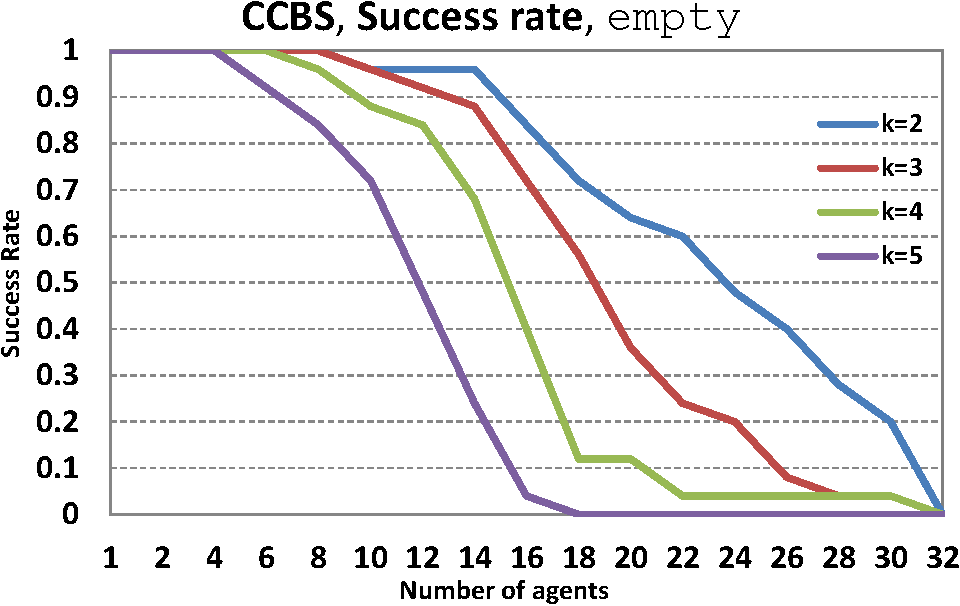
\includegraphics[width=0.45\linewidth]{mapfr-sr-plot-ccbs-empty.pdf}
        %\caption{}
        %\label{}
    \end{subfigure}\hspace{0.025\linewidth}%
    \begin{subfigure}
        \centering
        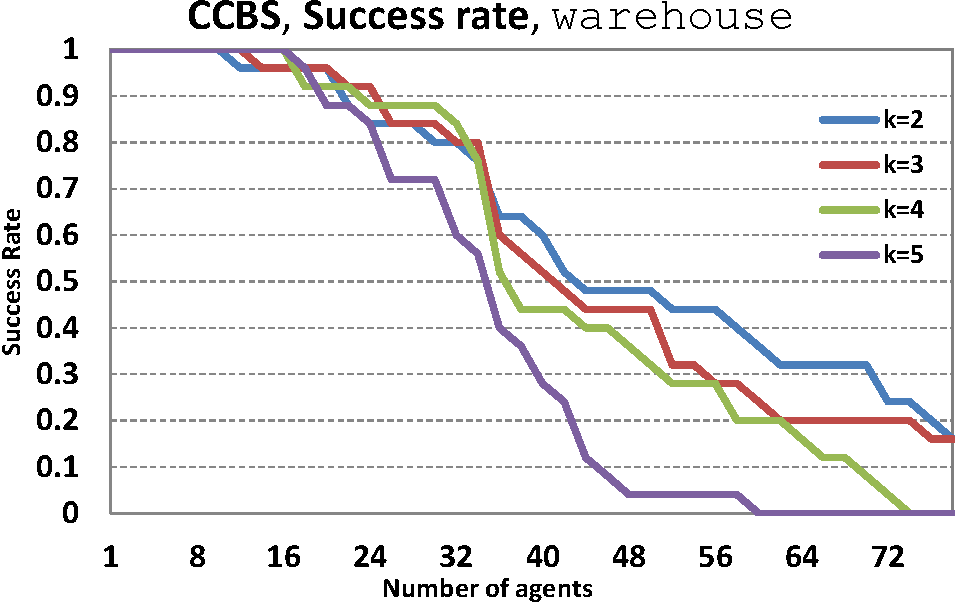
\includegraphics[width=0.45\linewidth]{mapfr-sr-plot-ccbs-warehouse.pdf}
        %\caption{}
        %\label{}
    \end{subfigure}
\end{subfigure}

\begin{subfigure}
    \centering
    \begin{subfigure}
        \centering
        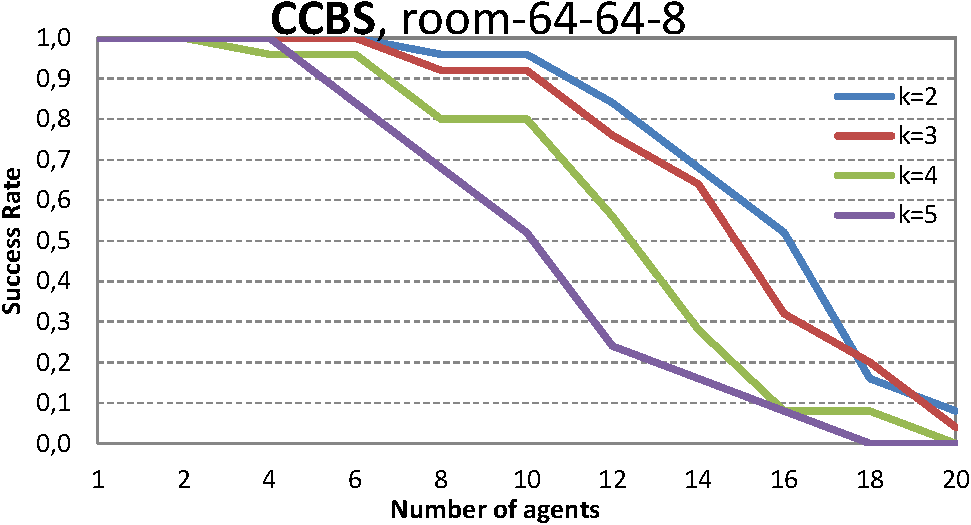
\includegraphics[width=0.45\linewidth]{mapfr-sr-plot-ccbs-room.pdf}
        %\caption{}
        %\label{}
    \end{subfigure}\hspace{0.025\linewidth}%
    \begin{subfigure}
        \centering
        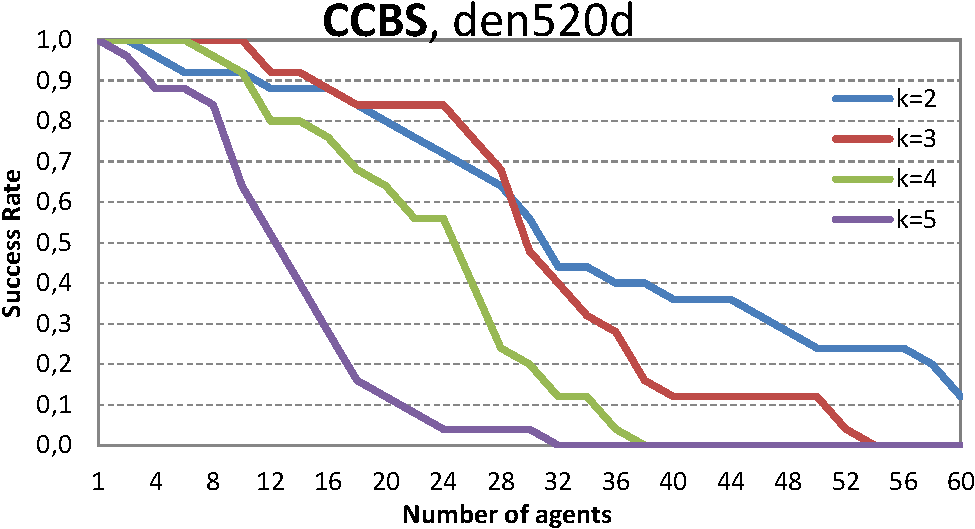
\includegraphics[width=0.45\linewidth]{mapfr-sr-plot-ccbs-den520d.pdf}
        %\caption{}
        %\label{}
    \end{subfigure}%\hspace{0.025\linewidth}%
\end{subfigure}

\caption{Success rate for \ccbs on grid maps.}
\label{fig:results-ccbs-SR-grids}
\end{figure*}

\begin{figure*}[t]
\centering
    \begin{subfigure}
        \centering
        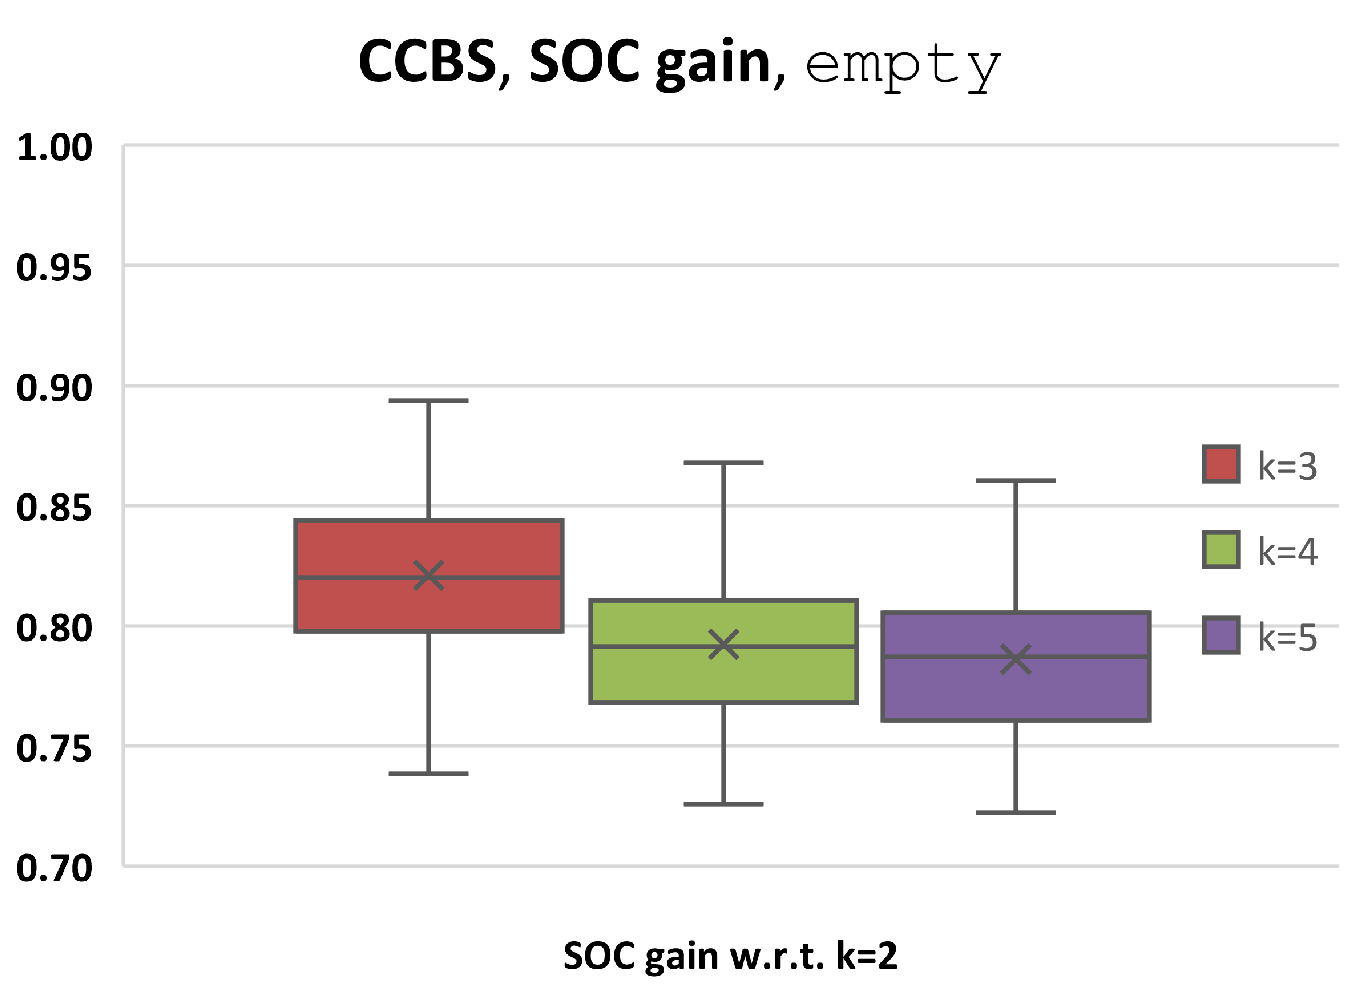
\includegraphics[width=0.45\linewidth]{mapfr-SOC-plot-ccbs-empty.pdf}
        %\caption{}
        %\label{}
    \end{subfigure}\hspace{0.025\linewidth}%
    \begin{subfigure}
        \centering
        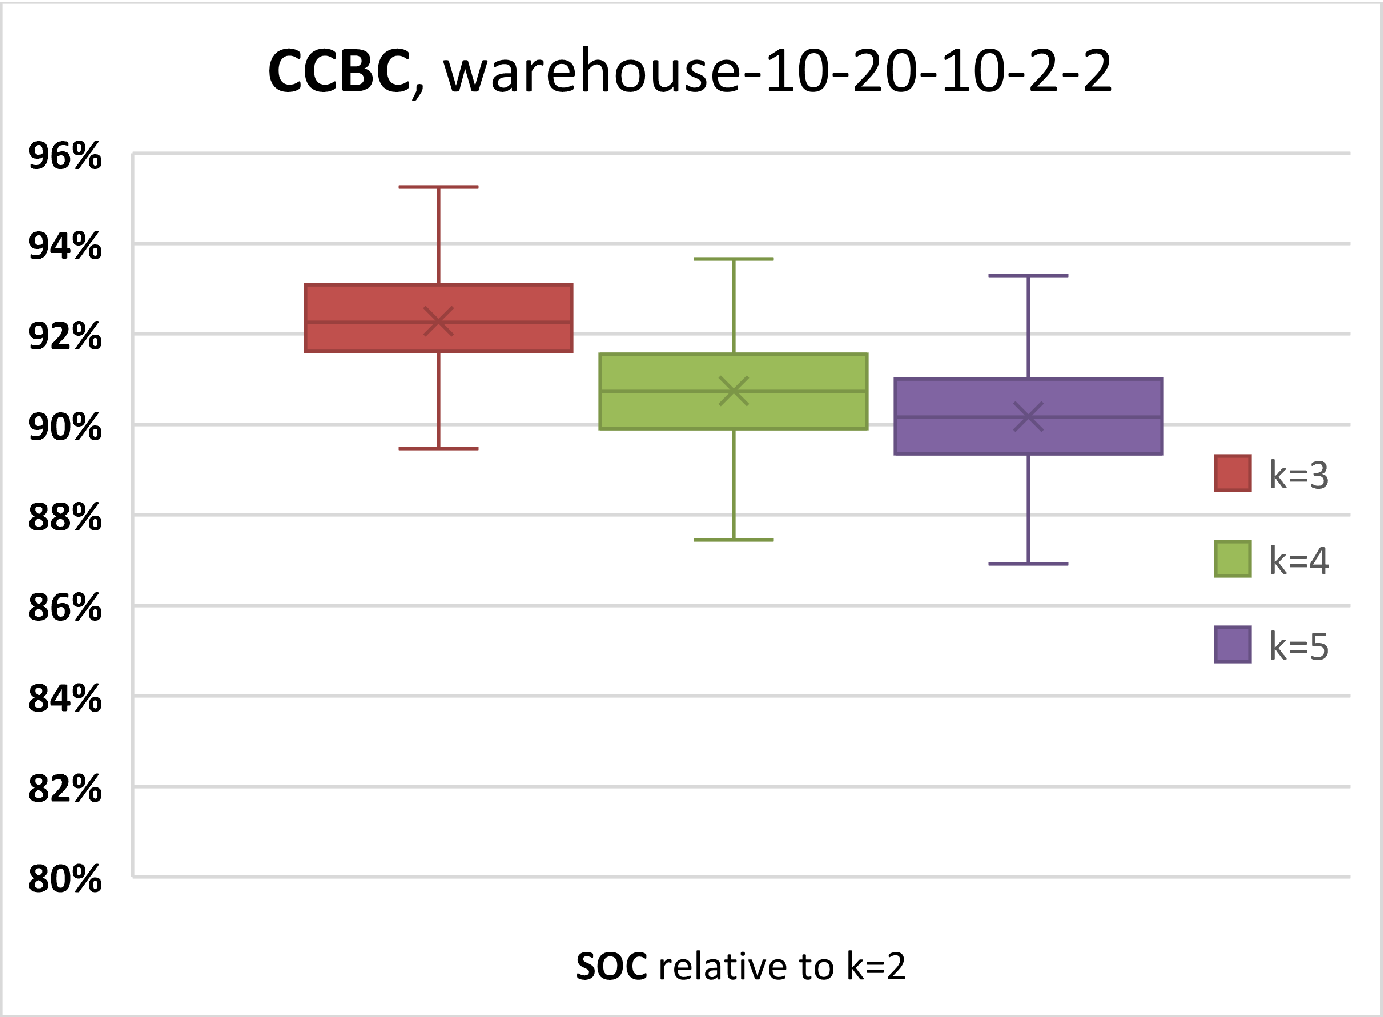
\includegraphics[width=0.45\linewidth]{mapfr-SOC-plot-ccbs-warehouse.pdf}
        %\caption{}
        %\label{}
    \end{subfigure}%\hspace{0.025\linewidth}%
    
    \begin{subfigure}
        \centering
        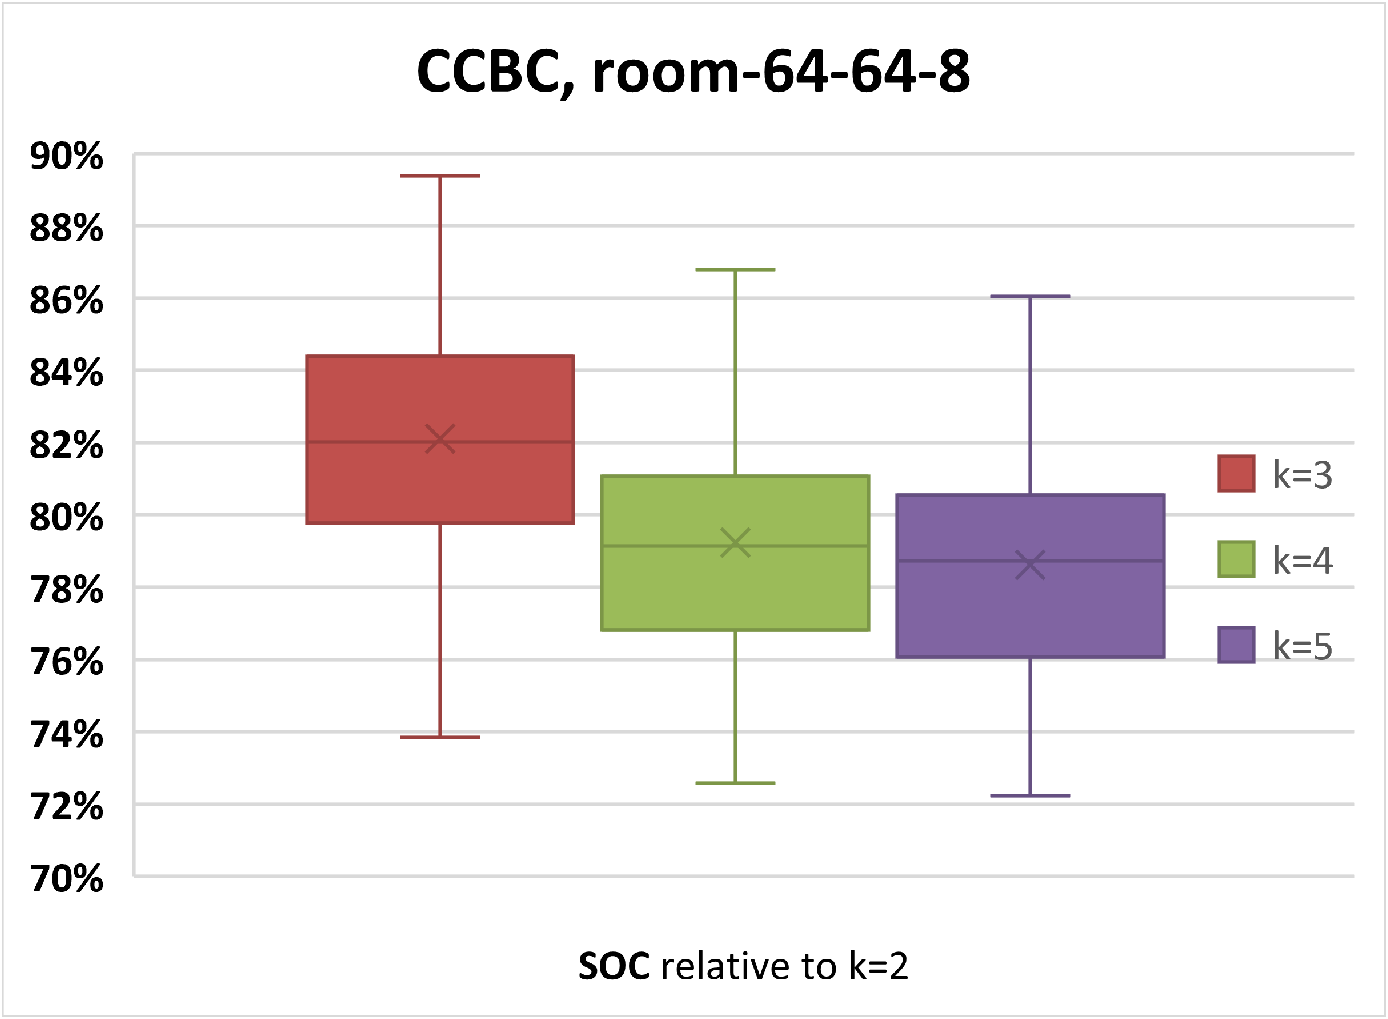
\includegraphics[width=0.45\linewidth]{mapfr-SOC-plot-ccbs-room.pdf}
        %\caption{}
        %\label{}
    \end{subfigure}\hspace{0.025\linewidth}
    \begin{subfigure}
        \centering
        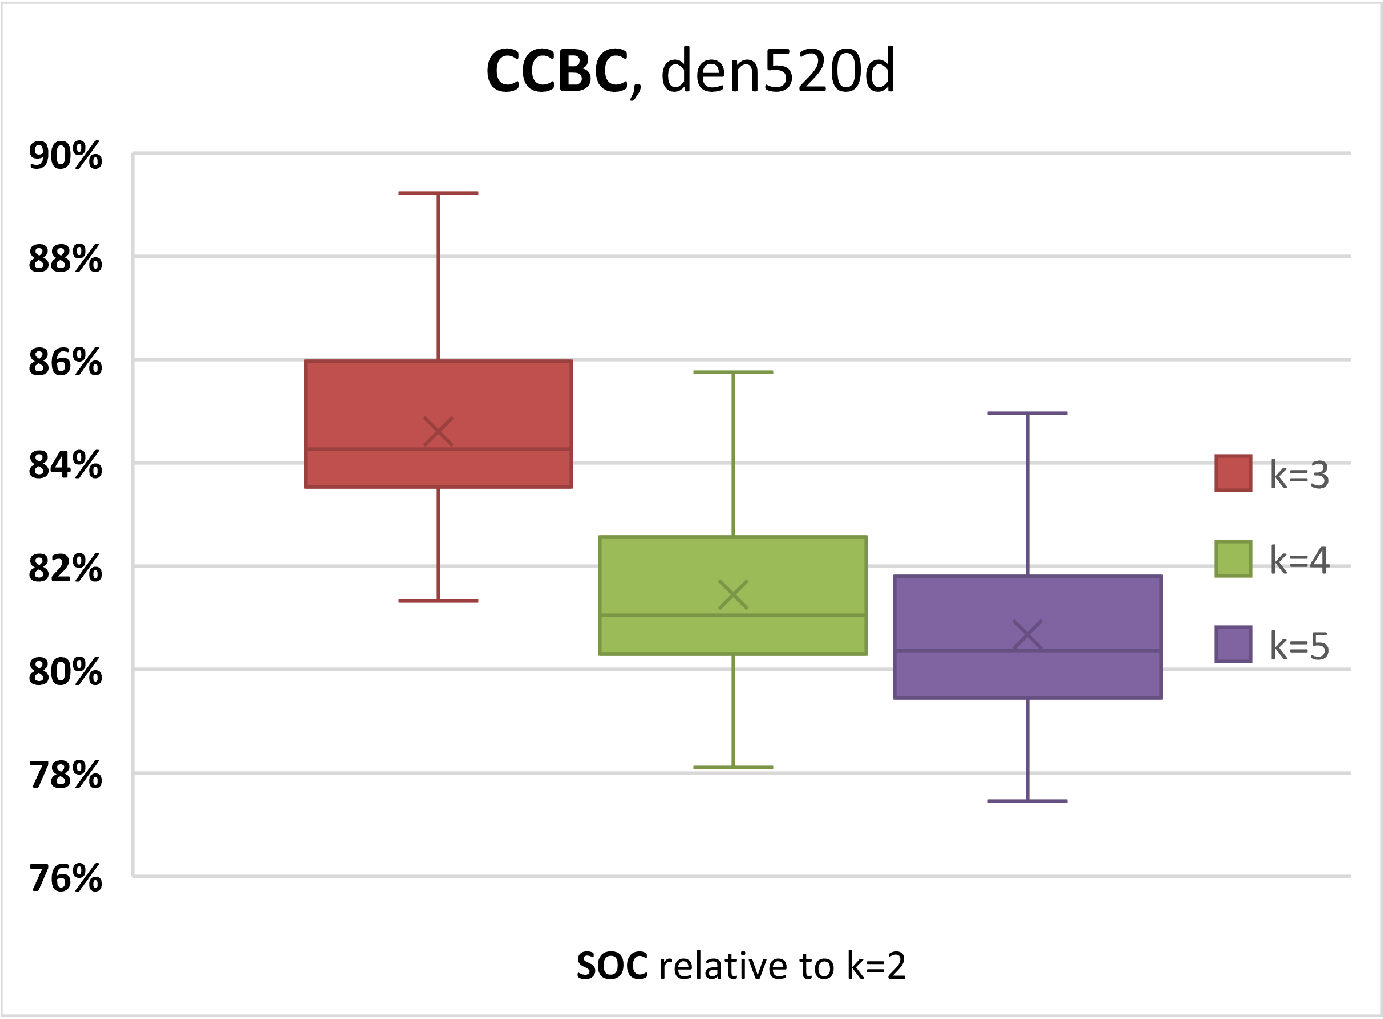
\includegraphics[width=0.45\linewidth]{mapfr-SOC-plot-ccbs-den520d.pdf}
        %\caption{}
        %\label{}
    \end{subfigure}%\hspace{0.025\linewidth}%
    
\caption{The SOC gain ratio between $k=3,4,5$ and $k=2$ for \ccbs on grid maps.}
\label{fig:results-ccbs-SOC-grids}
\end{figure*}


\subsection{\ccbs results}

Figure \ref{fig:results-ccbs-SR-grids} depicts the success rate of \ccbs on our grid graphs. Plots of different colors correspond to results for different values of grid connectivity, i.e., different values of $k$ for $2^k$-neighborhood grids. 


% It is working! 
The results show that our implementation of \ccbs can find SOC-optimal solutions under the 30 second time limit for \mapfr problems with several dozens of agents in some grids. 
For example, \ccbs solved 80\% of problems for 24 agents on the \texttt{warehouse} grid for all evaluated values of $k$ (2, 3, 4, and 5).


% Slower than classical 
Note that state-of-the-art \cbs variants 
%\konstantin{should not it be 'state-of-the-art'?} \roni{Fixed}
can find SOC-optimal solutions to classical \mapf problems on similar grids with many more agents. This is expected, since finding SOC-optimal solutions to classical \mapf problems is an easier task than finding SOC-optimal solutions to \mapfr problems, especially when imposing 30 seconds time limit. 

% Increasing k means slower
Consider now the impact of increasing the neighborhood size, i.e., increasing $k$. 
In general, the latter leads to lower success rates. This is an expected effect resulting from the difference in branching factor, which is $4$ for $k=2$ and goes up to $32$ for $k=5$. However, for some settings, higher values of $k$ may actually increase success rate. 
For example, the results in Figure~\ref{fig:results-ccbs-SR-grids} for \texttt{den520d} show that up to 30 agents, the success rate for $k=3$ was higher than the success rate for $k=2$.  
A possible explanation is that increasing $k$ also allows the agents to find shorter single-agent plans, which helps to speed up the search. In other words, increasing $k$ means a search space with a larger branching factor and a potentially smaller depth. %, but also having optimal solutions in shallower depth. where it decreases its depth. 


\subsubsection{The Impact of Grid Connectivity on SOC}
% SOC
Increasing $k$ has an additional, desirable effect: it decreases the SOC of the returned solution since increasing $k$ means additional possible move actions per location, which may allow agents to reach their goals earlier. To measure this effect, we computed for every solved \mapfr problem the ratio between the SOC of the returned solution and the SOC for $k=2$. 
We call this the \emph{SOC gain ratio}. 
If the SOC gain ratio is, for example, $0.75$, it means that the SOC of the returned solution is smaller that the one for $k=2$ by $25\%$. 
Figure~\ref{fig:results-ccbs-SOC-grids} shows the SOC gain ratio as box-and-whisker plots, for different values of $k$. Each plot shows the following statistics: minimum, maximum, median (horizontal line inside the box), mean (cross sign inside the box), and first and third quartiles. 

% Adding $k$ helpful, but only for small k
As one can see, increasing $k$ indeed decreases SOC. 
For example, in the grid \texttt{room-64-64-8}, the average SOC gain for $k=3, 4$ and 5 is 82.12\%, 79.23\%, and 78.62\%, respectively.
Note that the gain, in terms of SOC, exhibits a diminishing return effect. That is, going from $k=3$ to $k=4$ and from $k=4$ to $k=5$ provides less effect on SOC. In fact, in all our experiments going from $k=4$ to $k=5$ yielded a marginal improvement of approximately 1\% in SOC. %\roni{Marginal improvement in which statistics? i.e., is it 1\% improvement in the average? median? quartiles?}\konstantin{In all statistics, as I see from the plots.}


% Different grids
Consider now the different behavior of \ccbs on the different grids. 
When moving from $k=2$ and $k=3$, 
the average SOC decreased by 25\%, 25\%, 18\%, and 8\% for the grids \texttt{room-64-64-8}, \texttt{empty-16-16}, \texttt{den520d}, and \texttt{warehouse}, respectively. 
We conjecture that the gain was smaller for the \texttt{warehouse} grid because this grid has numerous prolonged passages -- corridors -- spanned in orthogonal directions. An agent moving in these corridors only uses the cardinal ($k=2$) moves. Thus, the only gain obtained by allowing other moves is due to the presence of open areas on the borders of the \texttt{warehouse} grid. 

%\roni{Edited the above. Let me know what you think} \konstantin{Great. Left some comments. We're almost there.}

%Going from $k=3$ to $k=4$ and from $k=4$ to $k=5$ provides less effect on SOC. For all maps the first transition infers $2-3\%$ difference and the second one - $1\%$ or less.


\begin{figure}
    \centering
    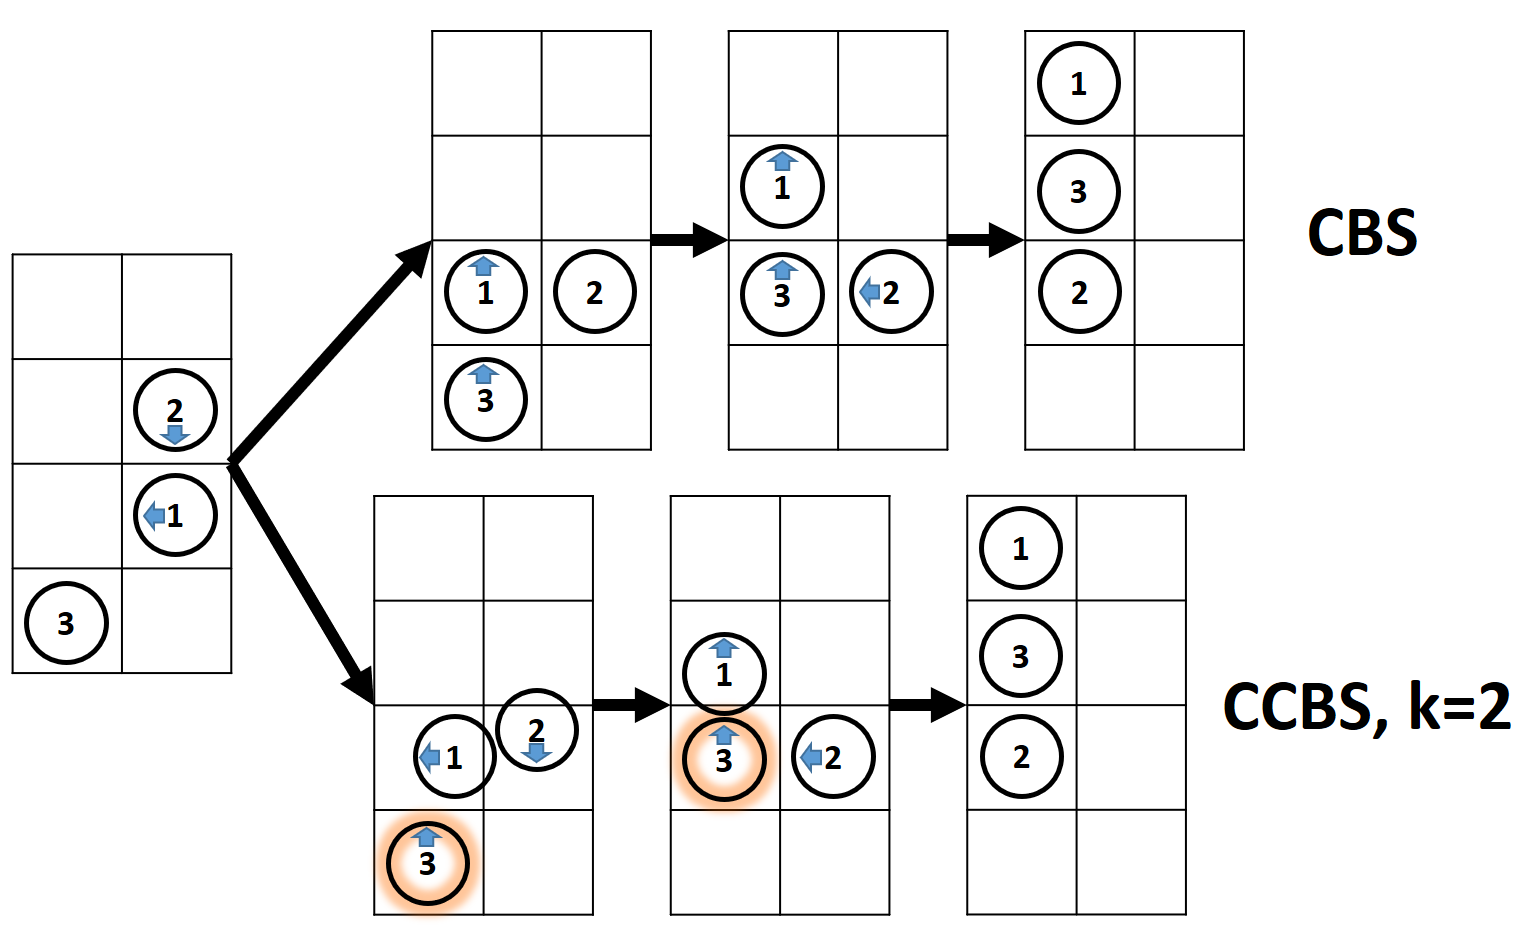
\includegraphics[width=0.7\columnwidth]{anton-example.PNG}
    \caption{Example: \ccbs for $k=2$ finds better solution than \cbs.}
    \label{fig:anton-example}
\end{figure}

% Something about the standard CBS
We also compared the performance of \ccbs with $k=2$ and a standard \cbs implementation. 
\cbs was faster than \ccbs, as its low-level solver is \astar on a 4-neighborhood grid, in which detecting collisions is trivial, and it has only unit-time wait actions. However, even for $k=2$, \ccbs is able, in some cases, to find better solutions, i.e., solutions of lower sum-of-costs. This is because, an agent may start to move after waiting less than a unit time step. 
Figure~\ref{fig:anton-example} illustrates an example of such scenario. An animation of this example is given in \url{https://tinyurl.com/ccbs-vs-cbs2}. %file \texttt{C-CBSvsCBS.gif} in the supplementary material. % shows an animation of this example. 




\subsubsection{Comparison to E-ICTS}


\begin{figure}
    \centering
    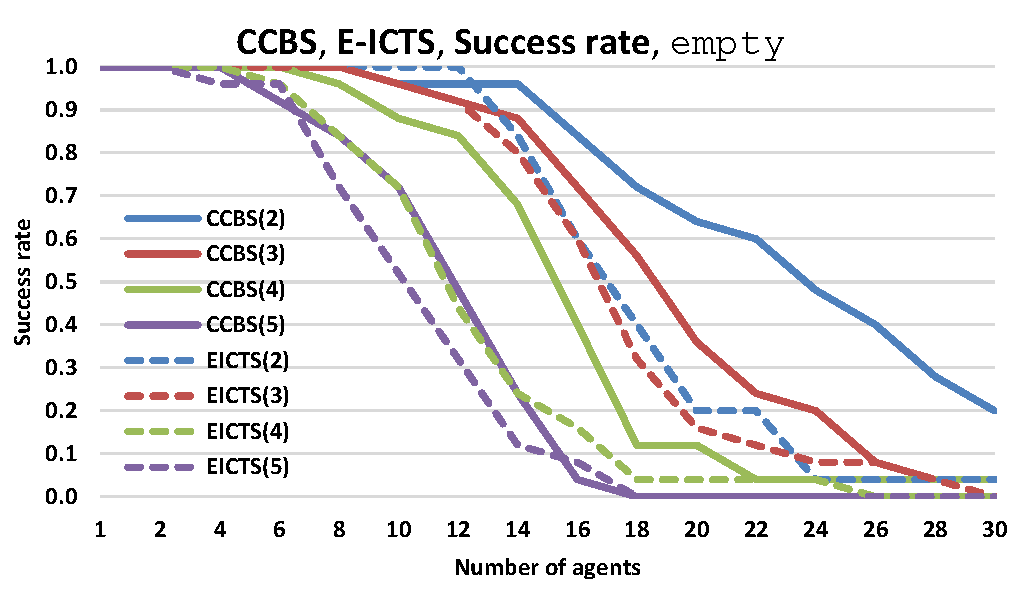
\includegraphics[width=0.75\columnwidth]{ccbs-eicts-sr-plot-empty_NEW.pdf}
    %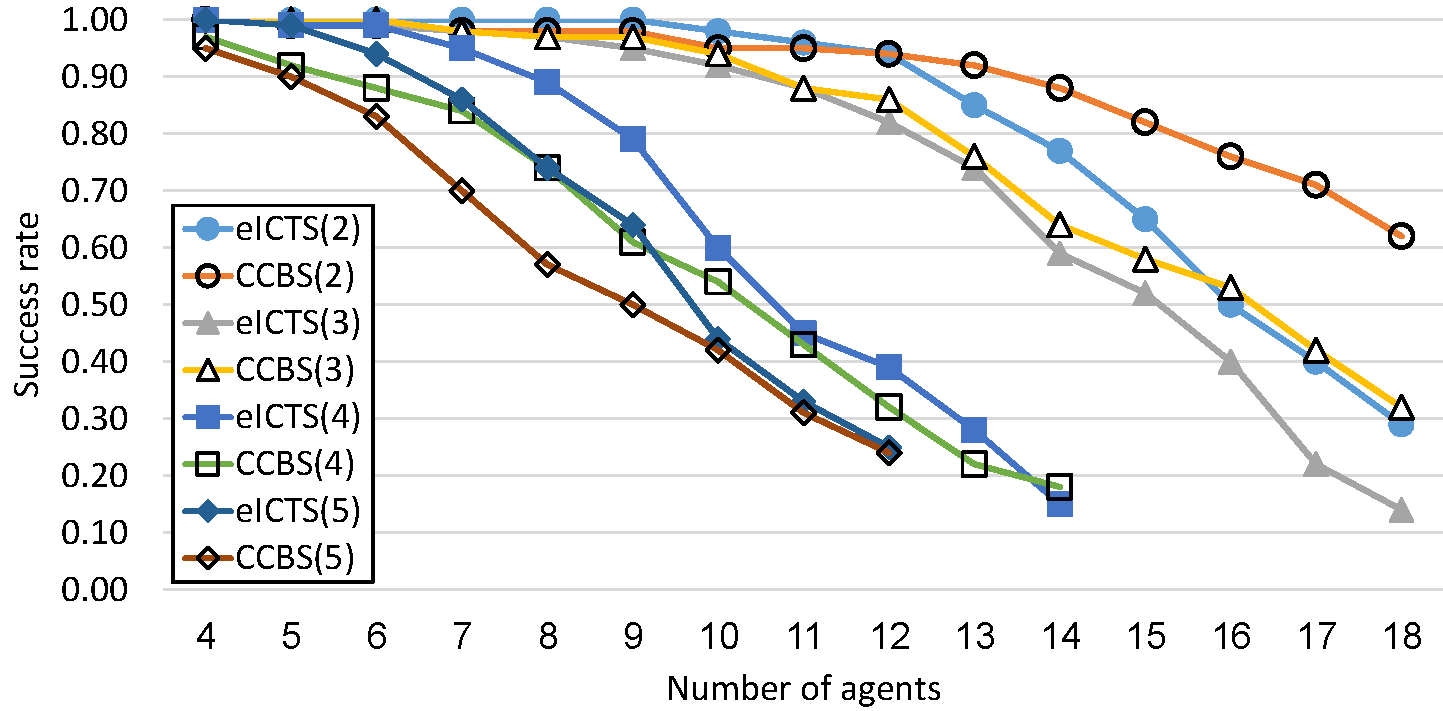
\includegraphics[width=0.85\columnwidth]{ccbsVsICTS_cropped.pdf}
    \caption{Success rate of \ccbs and E-ICTS in 16$\times$16 empty grid.}
    \label{fig:ccbs-vs-eicts}
    \vspace{-0.3cm}
\end{figure}


We compared the performance of \ccbs and E-ICTS~\cite{walker2018extended}, a \mapfr algorithm based on the Increasing Cost Tree Search (ICTS) framework~\cite{sharon2013increasing}. We thank the E-ICTS authors who made their implementation publicly available (\url{https://github.com/thaynewalker/hog2}.\footnote{E-ICTS code used in the experiments was downloaded from the authors' repository at January 2019.})

Like \ccbs, E-ICTS  can also handle non-unit edge cost. As for the time dimenstion, E-ICTS handles continuous time by discretizing it according to a minimal wait time parameter $\Delta$ (we set it to be 1/1000 in our experiments). Note that given an accurate unsafe interval detection mechanism, \ccbs handles continuous time directly, and thus can return better solutions than E-ICTS. However, the unsafe interval detection mechanism we implemented for this experiment did, in fact, discretize time with the same level of granularity, and so the comparison to E-ICTS is valid. 

Figure~\ref{fig:ccbs-vs-eicts} shows the success rate of the two algorithms on \texttt{empty} grid with different number of agents and $k=2, 3, 4,$ and 5. The results show that in most cases E-ICTS is outperformed by \ccbs. However for some combinations of $k$ and number of agents E-ICTS solved more instances, e.g. $k=2$ for 10-12 agents or $k=5$ for 6 agents.\footnote{Note that in our conference paper on \ccbs~\cite{andreychuk2019multi} we reported that \ccbs was outperformed by E-ICTS on a similar empty map for higher values of $k$. We hypothesize that the better performance of \ccbs now is because we improved our implementation of \ccbs. 
Moreover the time limit imposed in the experiments reported here was 30 seconds while it was 60 seconds for the conference paper.}
That being said, we note that the conducted evaluation considered different implementations of E-ICTS and \ccbs, and we do not presume to infer from this set of experiments when each algorithm is better. Identifying which \mapf algorithm to use in which domain is an open question even for classical \mapf.


\subsubsection{Roadmap Results}


\begin{figure}
\centering
    \centering
    
    \begin{subfigure}
        \centering
        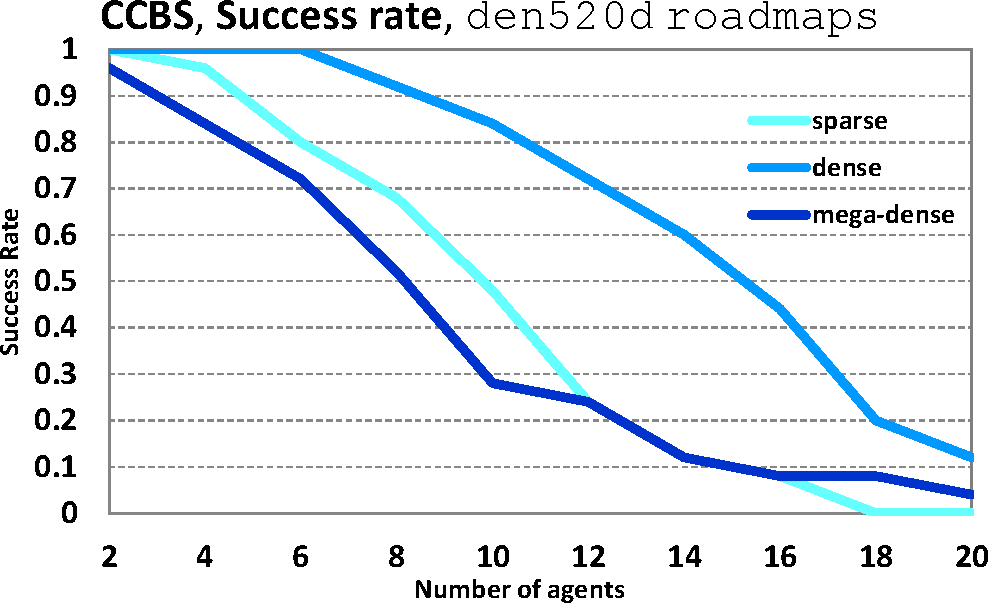
\includegraphics[width=0.45\linewidth]{mapfr-sr-plot-ccbs-den520d_roadmaps.pdf}
        %\caption{}
        %\label{}
    \end{subfigure}\hspace{0.025\linewidth}
    \begin{subfigure}
        \centering
        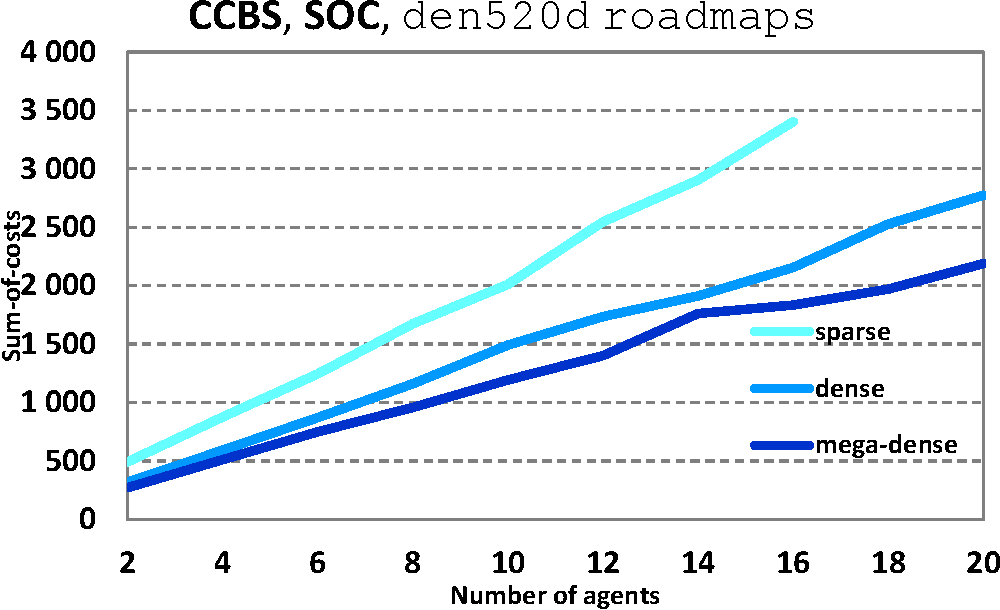
\includegraphics[width=0.45\linewidth]{mapfr-SOC-plot-ccbs-den520d_roadmaps.pdf}
        %\caption{}
        %\label{}
    \end{subfigure}%\hspace{0.025\linewidth}%
    
    \caption{\ccbs success rate and SOC for different roadmaps.}
    \label{fig:results-ccbs-SR-SOC-roadmaps}
\end{figure}

Fig.~\ref{fig:results-ccbs-SR-SOC-roadmaps} depicts the success rates (left) and SOC (right) for \ccbs on the roadmap graphs. 
%The success rate of \ccbs on roadmap graphs is lower compared to grids. \roni{Why?} \konstantin{I think it's because of the number of reasons. The most evident is that the tasks are different in the scenarios (so they are not directly comparable, actually) and the number of scenarios is small (thus, if we take other scenarios for grids and/or roadmaps we will see different figures).}
%\roni{I agree they are not comparable. So, I'd remove this text that compared the roadmap results with the grid results.} \konstantin{Agree. btw, it seems like an appealing direction for future work - analyzing the behaviour of CCBS on roadmaps.}\roni{Yes, the fact that we can run on roadmaps does not mean we are doing it in the best way possible. Definitly worth thinking. But, I think maybe stronger to think about how to intergrate a dynamic way to create the roadmap, specifically for MAPF. E.g., add more edges only when you have a conflict. But, future work, let's submit first:)}
%\roni{I went along and commented this out}

Observe that the behavior of \ccbs in terms of success rate is similar for the \texttt{sparse} and \texttt{mega-dense} graphs while the success rate is notably higher for \texttt{dense} roadmap. This can be explained as follows. On the \texttt{sparse} graph the number of edges is low thus many agents may plan to use the same edges. Thus, numerous conflicts arise making the problem harder for \ccbs. On the other hand, when the number of edges is very high, like in \texttt{mega-dense}, there are many ways to resolve a conflict. I.e., \ccbs can select one of the numerous alternative edges to perform a move action. However, edges of this roadmap are compactly embedded into the metric space, so by choosing an alternative edge the conflict is not eliminated in a sense that another conflict immediately arises in the vicinity of the old one. Thus, the overall number of conflicts is big and \ccbs can not process them all within the time limit. Setting a moderate number of edges (not too low and not too high), like in the \texttt{dense} setting, seems to provide a reasonable trade-off between the number of possible detour options and the density of edges, yielding a notably higher success rate.

The right-hand side of Figure~\ref{fig:results-ccbs-SR-SOC-roadmaps} shows the average SOC obtained for different number of agents and types of graphs. Here we observe a monotonic impact of graph density on the SOC of the returned solution. The average SOC for \texttt{sparse} is larger than for \texttt{dense} which is larger than the average SOC for \texttt{mega-dense}. 
This difference in SOC is because %when agents have fewer edges to follow, they have more opportunity to conflict. 
when the number of edges increases, agents are likely to have more options to reach their goals without substantial spatial detours, which yields lower SOC. 
Here too we observe diminishing return effect, where increasing the number of edges in the graph yields a smaller advantage as the graph becomes more dense. This can be seen when comparing the SOC of \texttt{dense} and \texttt{mega-dense}.
The SOC for the \texttt{sparse} roadmap is on average $48\%$ larger than for the \texttt{dense} roadmap, and the latter is on average $18\%$ larger than for the \texttt{mega-dense}.
This suggests that moderately dense roadmap representations of the environment are beneficial when solving \mapfr with \ccbs, as they positively influence the success rate and the advantage in terms of SOC of denser roadmaps is limited.

\subsection{\smtccbs results}

\begin{figure*}[h]
\centering
\begin{subfigure}
    \centering
    \begin{subfigure}
        \centering
        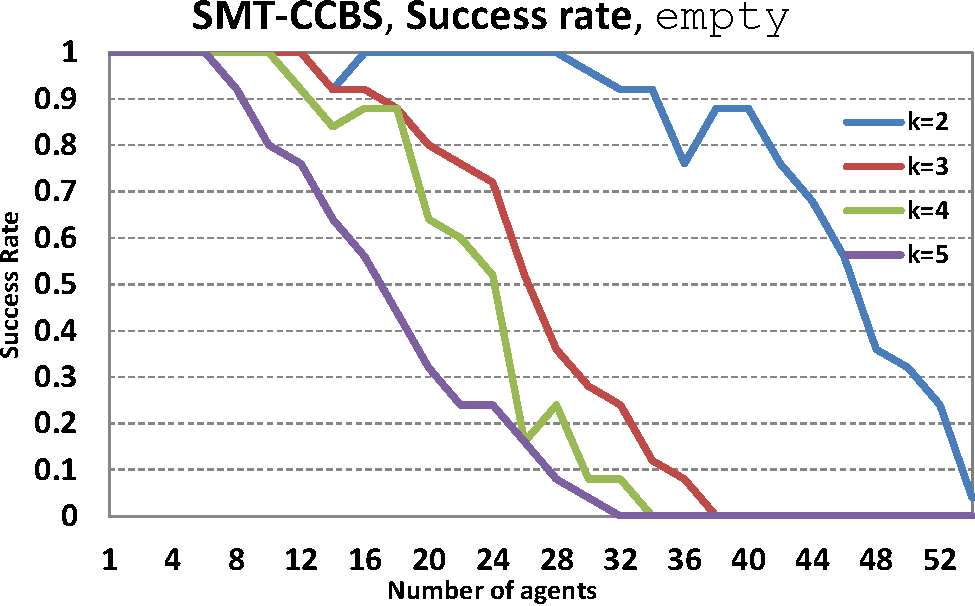
\includegraphics[width=0.45\linewidth]{mapfr-sr-plot-smtcbs-empty.pdf}
        %\caption{}
        %\label{}
    \end{subfigure}\hspace{0.025\linewidth}
    \begin{subfigure}
        \centering
        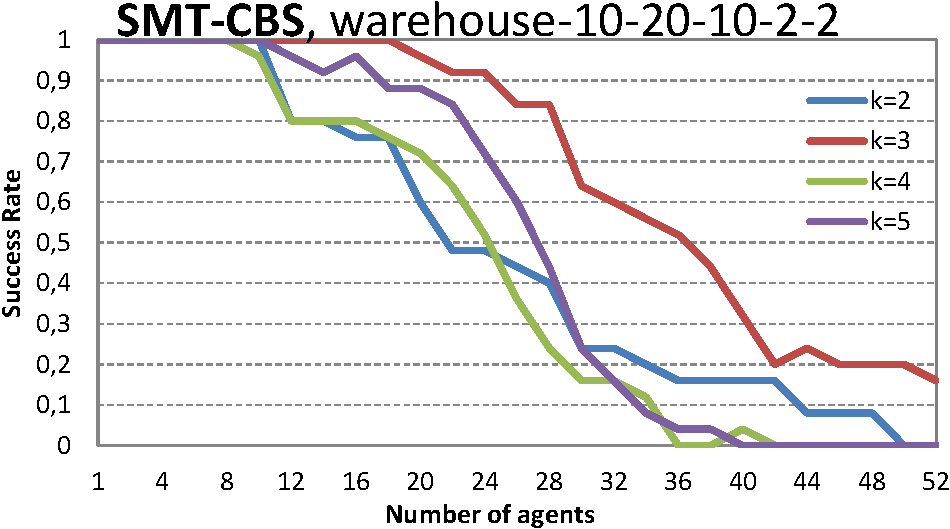
\includegraphics[width=0.45\linewidth]{mapfr-sr-plot-smtcbs-warehouse.pdf}
        %\caption{}
        %\label{}
    \end{subfigure}%\hspace{0.025\linewidth}
\end{subfigure}

\begin{subfigure}
    \centering

    \begin{subfigure}
        \centering
        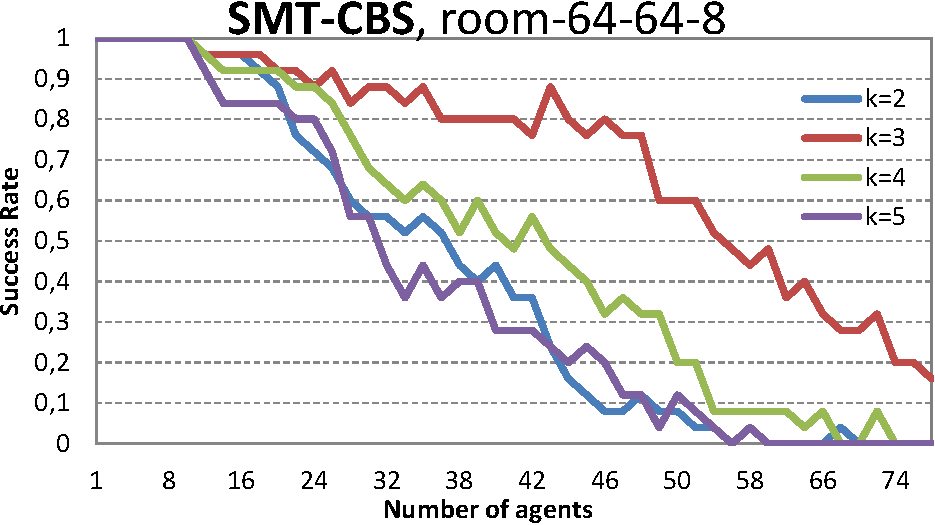
\includegraphics[width=0.45\linewidth]{mapfr-sr-plot-smtcbs-room.pdf}
        %\caption{}
        %\label{}
    \end{subfigure}\hspace{0.025\linewidth}
    \begin{subfigure}
        \centering
        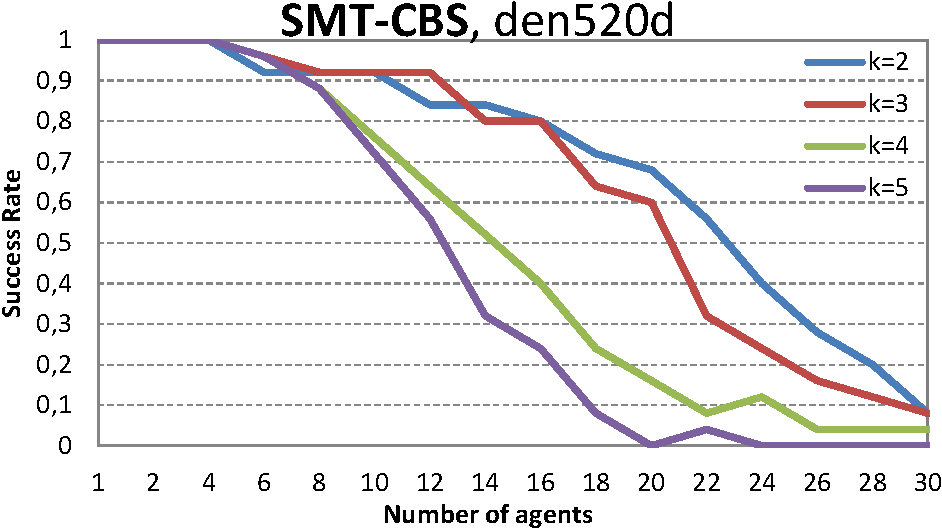
\includegraphics[width=0.45\linewidth]{mapfr-sr-plot-smtcbs-den520d.pdf}
        %\caption{}
        %\label{}
    \end{subfigure}%\hspace{0.025\linewidth}
\end{subfigure}

\caption{Success rate for \smtccbs on grid maps.}
\label{fig:results-success-rate-smtcbs-grids}
\end{figure*}

\begin{figure*}[t]
\centering
    \begin{subfigure}
        \centering
        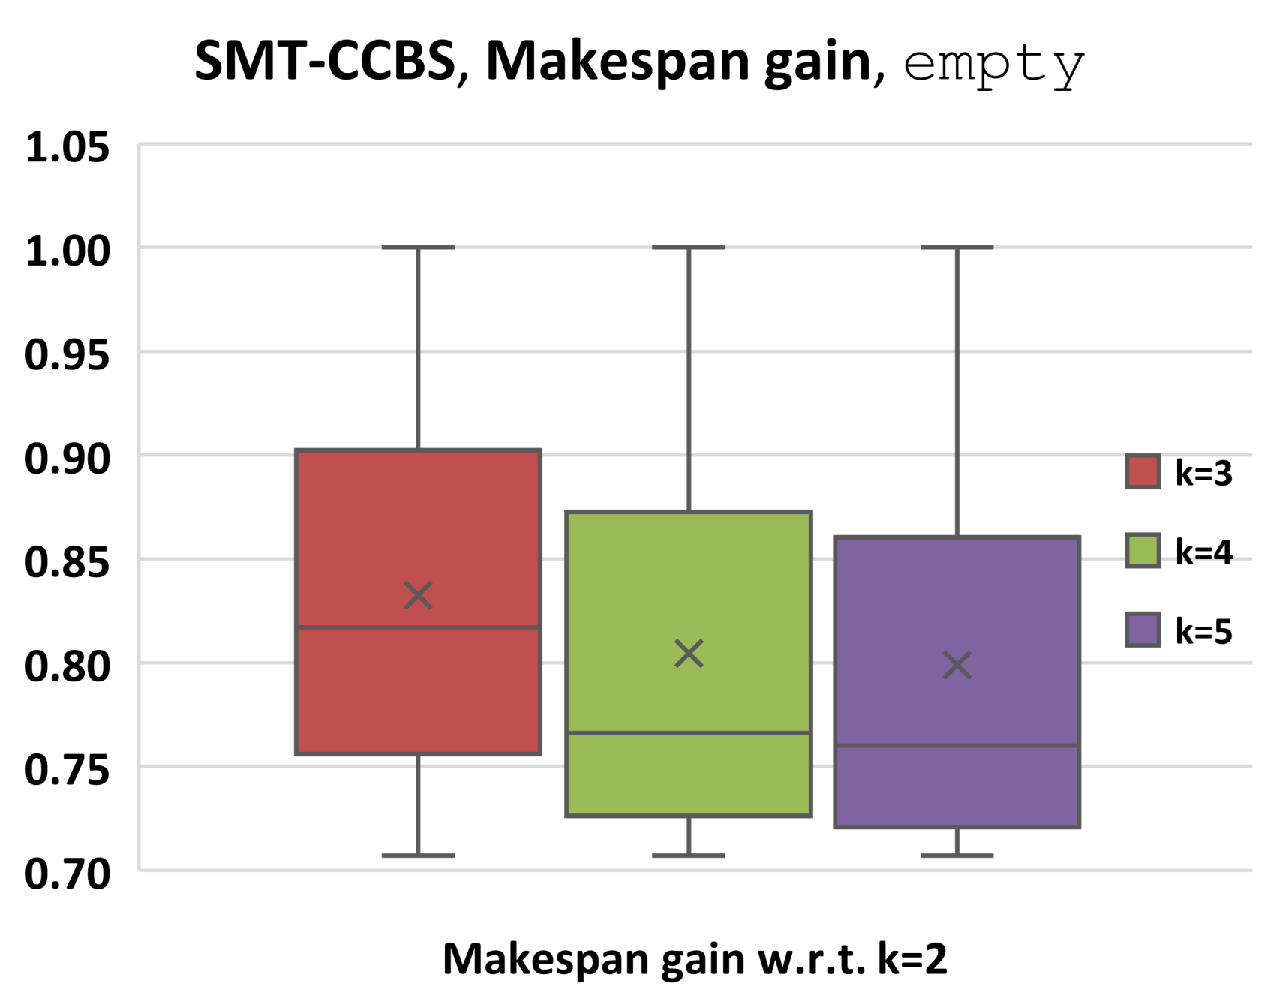
\includegraphics[width=0.45\linewidth]{mapfr-Makespan-plot-smtcbs-empty.pdf}
        %\caption{}
        %\label{}
    \end{subfigure}\hspace{0.025\linewidth}%
    \begin{subfigure}
        \centering
        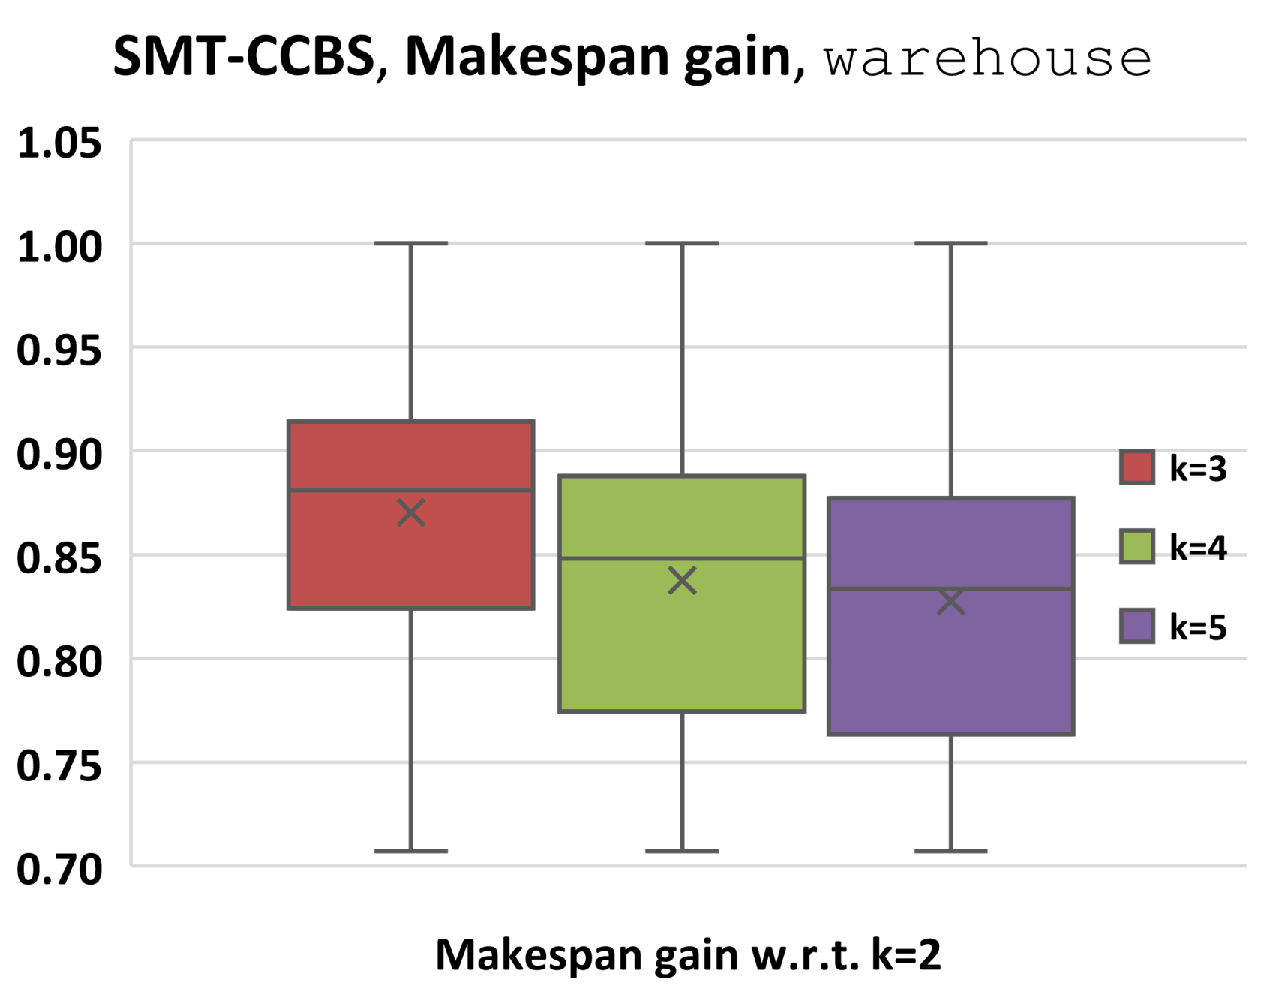
\includegraphics[width=0.45\linewidth]{mapfr-Makespan-plot-smtcbs-warehouse.pdf}
        %\caption{}
        %\label{}
    \end{subfigure}%\hspace{0.025\linewidth}%
    
    \begin{subfigure}
        \centering
        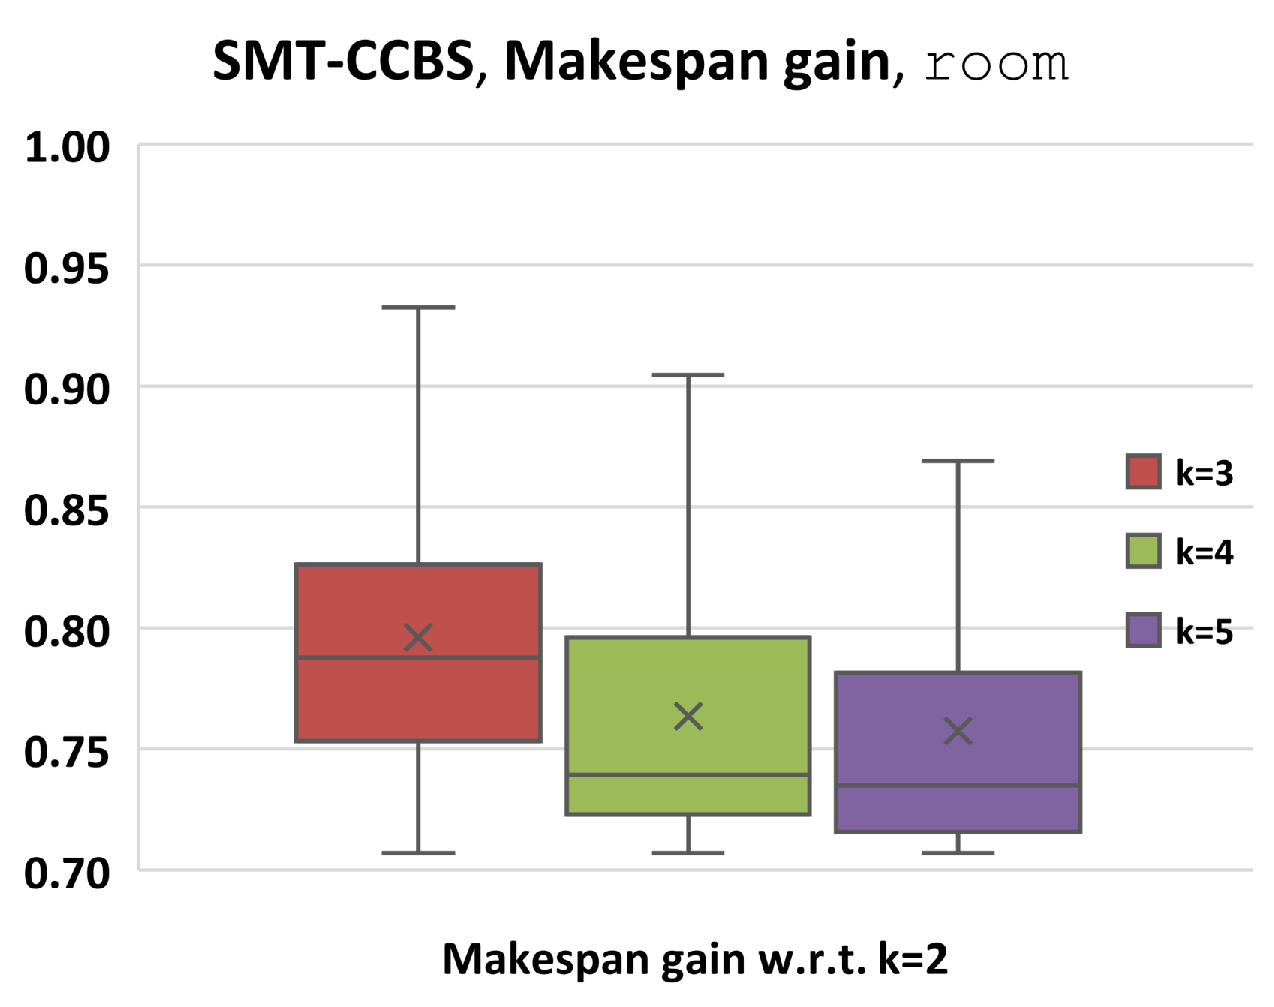
\includegraphics[width=0.45\linewidth]{mapfr-Makespan-plot-smtcbs-room.pdf}
        %\caption{}
        %\label{}
    \end{subfigure}\hspace{0.025\linewidth}
    \begin{subfigure}
        \centering
        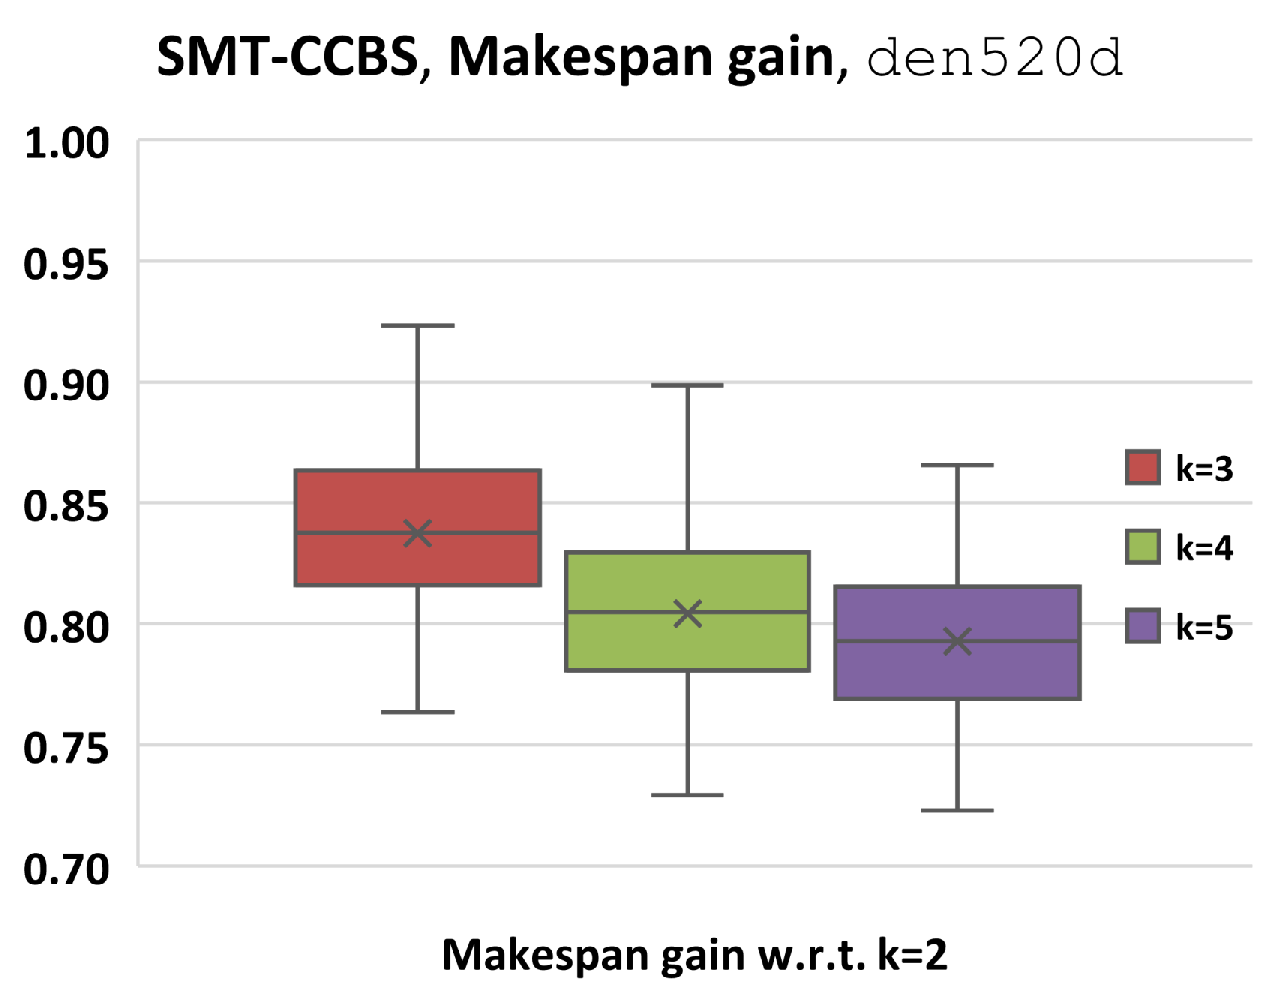
\includegraphics[width=0.45\linewidth]{mapfr-Makespan-plot-smtcbs-den520d.pdf}
        %\caption{}
        %\label{}
    \end{subfigure}%\hspace{0.025\linewidth}%
    
\caption{The makespan gain for $k=3,4,5$ w.r.t. $k=2$ for \smtccbs on grid maps.}
%\roni{Please make sure the y-axis is the same in all 4 plots, to allow comparison}} Thanks!
\label{fig:results-smtcbs-makespan-grids}
\end{figure*}



Next, we present our experimental results for \smtccbs. While we evaluated \smtccbs using the same experimental setup as in the \ccbs experiments described above, we intentionally avoid directly comparing \smtccbs and \ccbs. 
This is because \smtccbs and \ccbs are based on very different implementations, and more importantly are aimed to optimizie different objectives: \ccbs finds SOC-optimal solutions, while \smtccbs finds makespan-optimal solutions. 

Figure \ref{fig:results-success-rate-smtcbs-grids} depicts the success rate of \smtccbs for grid graphs \texttt{empty}, \texttt{room}, \texttt{warehouse}, and \texttt{den520d}. 
Plots of different colors correspond to different values of grid connectivity ($k$). Interestingly, the impact of $k$ on success rate depends largely on the map. Setting $k=2$ leads to the best results for \texttt{empty} and \texttt{den520d}, but not for \texttt{room} and \texttt{warehouse}. On the latter maps \smtccbs with $k=2$ performed very poorly, while the best results were provided with $k=3$. Moreover, on the \texttt{warehouse} map $k=2$ was outperformed by $k=5$ when the number of agents was up to 30, and on the \texttt{room} map -- by $k=4$ for up to 74 agents. Observing this, we hypothesize that higher connectivity helps in situations when agents must go through multiple way-points such as doors (for \texttt{room} map) or corridors (for \texttt{warehouse} map), surrounded by large portions of open space. This might be explained by a combination of two factors. First, having a highly connected neighborhood could help agents traverse open spaces using plans with fewer longer actions (which exists in higher $k$ values), which might be easier to find. Second, higher connectivity might help agents to coordinate their passing through the way-point due to better maneuverability before and after the way-point. This role of way points is further supported by the fact that we do not observe better success rate for higher $k$ in the \texttt{empty} map consisting of large single open space without any need to go through any way-point.

Relating the \smtccbs results to \ccbs results one can note the following. First, it appears that the performance of \smtccbs is apparently better for \texttt{empty} and \texttt{room} settings, while \ccbs shows better results for \texttt{warehouse} and \texttt{den520d}. One possible explanation for this is that SAT solvers are often good in solving formulae containing certain symmetries or being structured. Such structure could be inherited in the formula from the symmetric structure of the map (\texttt{room}) or from large empty spaces on the map (\texttt{empty}). Apparently, With increasing size of the map (\texttt{den520d}) the performance of \smtccbs decreases proportionally despite the helpful structure.
Second, \smtccbs was able in numerous cases to solve an instance with $n$ agents while not solving the same instance with $n-1$ agents. Thus, adding extra agents might be beneficial for \smtccbs, while this never happened to \ccbs. We hypothesize that the main reason for \smtccbs to exhibit such behaviour is that adding an agent does not necessarily increase the optimal makespan compared to the instance without the added agent. In such case, \mddrs for the same makespan bound will be of similar size and hence also the resulting formula will not be significantly larger for the instance with the added agent. Therefore underlying formulae for few consecutive numbers of agents could be of similar difficulty eventually enabling the observed fluctuations as it is known that SAT solvers  might intrinsically guess the solution fast for some formulas (corresponding to the instances with more agents in our case) while spend more time on solving other formulas of the similar size (corresponding to the instances with fewer agents in our case).




\subsubsection{The Impact of Grid Connectivity on Makespan with \smtccbs}
Figure \ref{fig:results-smtcbs-makespan-grids} shows the makespan gains of solutions generated by \smtccbs on grid maps.

As we can see, on average makespan monotonically decreases for increasing $k$ across all types of grid maps as enlarging the neighborhood gives the algorithm opportunity for finding shorter individual plans for agents, i.e. shorter overall makespan.
The resulting makespan gain seems to be mostly affected by extent of developing the connectivity for higher $k$. Open space in the grid supports higher connectivity while obstacles on the other hand limits it. Results supports this hypothesis, we can observe high makespan gain on \texttt{empty}, \texttt{room}, and \texttt{den520d} maps all with large open spaces while the lowest makespan gain is observed on the \texttt{warehouse} map that can has large obstacles in the middle.

Since the makespan is defined as the length of longest temporal plan from temporal plans of individual agents, it is less likely to change than SOC after adding an agent or changing the connectivity of the environment due to higher $k$. This is actually observed in some scenarios for \texttt{empty} and \texttt{warehouse} maps with no makespan gain after increasing $k$ (see the upper whisker in respective plots in Figure~\ref{fig:results-smtcbs-makespan-grids}).

\subsubsection{\smtccbs on Roadmaps}
Figure \ref{fig:results-smtccbs-SR-Makespan-roadmaps} shows success rate and makespan  results of \smtccbs for roadmaps. The makespan is computed per each number of agents from solution of scenarios solved under the given timeout.

We can see in Figure \ref{fig:results-smtccbs-SR-Makespan-roadmaps} that success rate of \smtccbs monotonically decreases for all number of agents with increasing the density of the roadmap graph. It case of \smtccbs it is expected, as it is more time consuming to process significantly larger graphs and solving correspondingly larger formulae containing more variables and constraints. The effect of increasing density of edges in case of roadmaps is multiplied by the absence of compression at the level of \mddr as in the roadmaps the symmetry of the neighborhood of a position is completely removed and  a possibility of generating a single node in \mddr by different paths is eliminated.

Notably these results, again, highlight the difference in between \ccbs and \smtccbs, as for \ccbs the roadmap with the smallest number of nodes and edges, i.e. \texttt{sparse}, was not the easiest to solve (as shown and explained before).

\begin{figure}
\centering
    \centering
    
    \begin{subfigure}
        \centering
        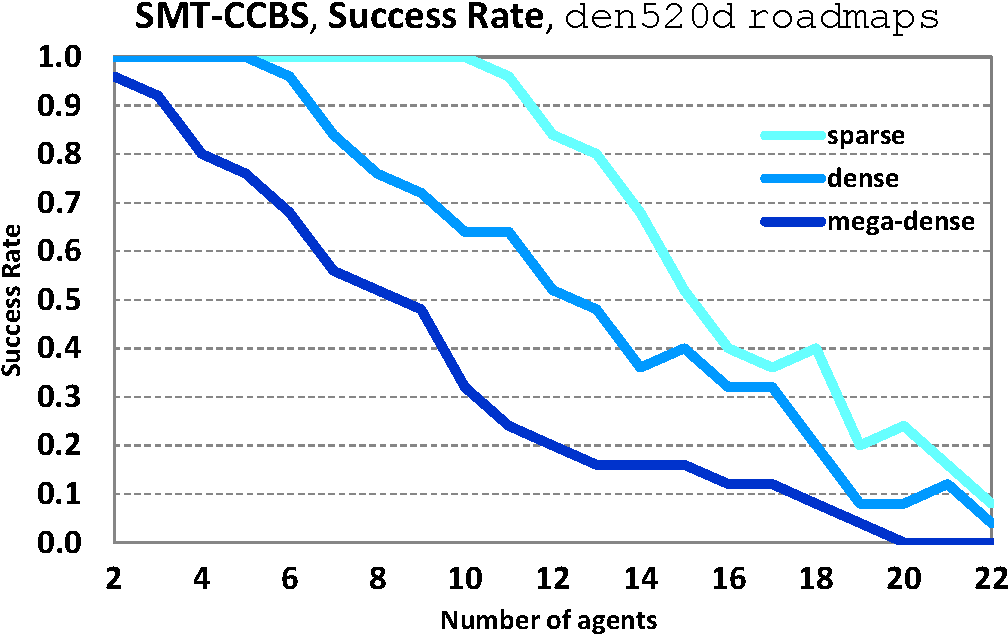
\includegraphics[width=0.45\linewidth]{mapfr-sr-plot-smtcbs-den520d_roadmaps.pdf}
        %\caption{}
        %\label{}
    \end{subfigure}\hspace{0.025\linewidth}
    \begin{subfigure}
        \centering
        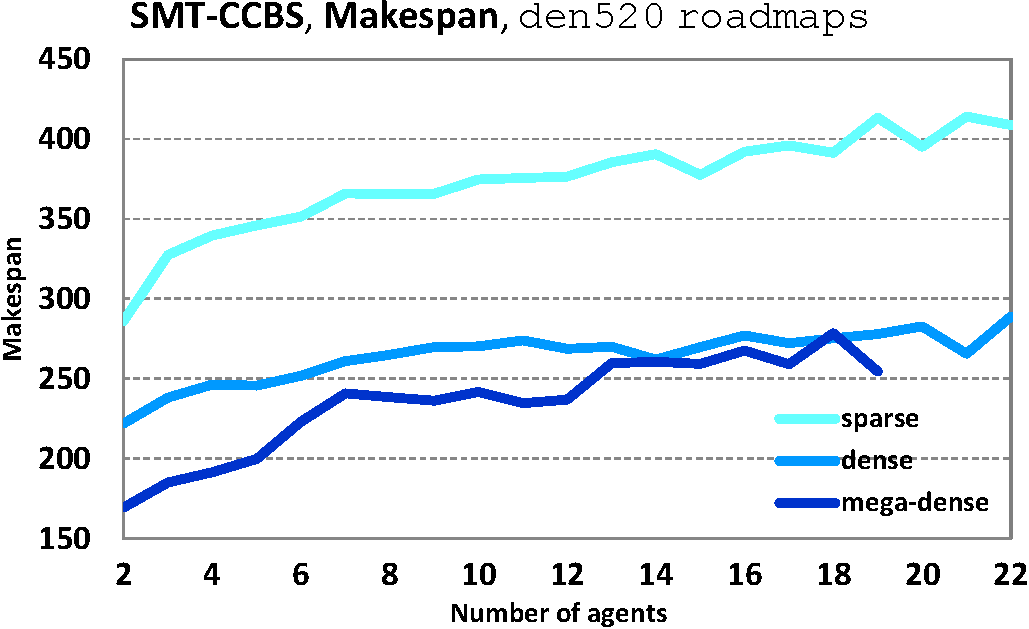
\includegraphics[width=0.45\linewidth]{mapfr-Makespan-plot-smtcbs-den520d_roadmaps.pdf}
        %\caption{}
        %\label{}
    \end{subfigure}%\hspace{0.025\linewidth}%
    
    \caption{\smtccbs success rate and makespan for different roadmaps.}
    \label{fig:results-smtccbs-SR-Makespan-roadmaps}
\end{figure}

%\pavel{Will we use roadmap results for \smtcbs ?}
%\konstantin{Yes. I inserted the plots.}

%Figure \ref{fig:results-smtccbs-SR-Makespan-roadmaps} shows success rate and makespan results of \smtccbs for roadmaps. The makespan is computed per each number of agents from scenarios solved under the timeout.
The right-hand side of Figure~\ref{fig:results-smtccbs-SR-Makespan-roadmaps} shows the average makespan obtained for different number of agents and types of graphs. Presumably, increasing the density of the graph positively influences makespan (the same trend was observed before for sum-of-costs). However, the difference between \texttt{dense} and \texttt{mega-dense} roadmaps in terms of makespan for number of agents exceeding 14 is negligible. It is also noteworthy, that although increasing number of agents results in longer makespan, the depicted curves are non-monotonic. This is causes caused by not having all instances solved within the time cap. If we ignore the timeout and wait for finishing all scenarios then the curve would be monotonic.

Overall, one again can claim that moderately dense roadmap representations of the environment are beneficial when solving \mapfr optimally w.r.t. makespan, as they positively influence the success rate and the advantage in terms of makespan is limited for denser roadmaps. However for \smtccbs, unlike \ccbs, there is also an option to decrease the size of the graph, i.e. make it more sparse, to trade-off solution cost for success rate.

% END COPY AND PASTE FROM WORKSHOP PAPER

\section{Related Work}
\label{sec:related-work}
%TODO: Roni
%Works related to us but not needed to explain our approach


\begin{table}[h]
%\begin{minipage}{\columnwidth} % so footnote will appear
\centering
\resizebox{0.85\columnwidth}{!}{
\begin{tabular}{@{}lccccccc@{}}
\toprule
\multicolumn{1}{c}{}                                           & \multicolumn{3}{c}{Actions} & Agent     &      &   &    \\ \midrule
\multicolumn{1}{c}{}                                           & N.U.         & Cont.         & Ang. & Vol. & Complete & Opt. & Dist. \\ \midrule
CBS-CT~\cite{cohen2019optimal} & \cmark   & \cmark & \cmark & \cmark & \cmark & \cmark & \xmark\\
E-ICTS~\cite{walker2018extended} & \cmark & \xmark             & \cmark    & \cmark  & \cmark  & \cmark    & \xmark     \\
AA-SIPP($m$)~\cite{yakovlev2017anyAngle} & \cmark            & \cmark             & \cmark    & \cmark    & \xmark & \xmark    & \xmark     \\
MCCBS~\cite{li2019multi} & \xmark            & \xmark             & \xmark    & \cmark  & \cmark  & \cmark    & \xmark     \\
CBS-CL\cite{walker2017using}  & \cmark    & \xmark    & \xmark    & \xmark  & \cmark  & \xmark    & \xmark     \\
%M*~\cite{wagner2015subdimensional} & \cmark            & \xmark             & \cmark    & \xmark  & \cmark  & \cmark    & \xmark     \\
MAPF-POST~\cite{honig2016multi,honig2017summary} & \cmark            & \cmark             & \cmark    & \cmark  & \cmark  & \xmark    & \xmark     \\
ORCA~\cite{snape2011hybrid}, ALAN~\cite{godoy2018alan} & \cmark            & \xmark             & \cmark    & \cmark & \xmark   & \xmark    & \cmark     \\
dRRT*~\cite{shome2020drrt} & \cmark            & \cmark             & \cmark    & \cmark & \cmark   & \xmark    & \xmark     \\
\ccbs~\cite{andreychuk2019multi} and \smtccbs~\cite{DBLP:conf/socs/Surynek19} & \cmark            & \cmark             & \cmark    & \cmark & \cmark    & \cmark    & \xmark     \\
 \bottomrule
\end{tabular}
}
%\end{minipage}
\caption{Overview: \ac{MAPF} research beyond the basic setting.}
\label{tab:related-work}
\end{table}
% START COPY AND PASTE FROM WORKSHOP PAPER


% Some prior work
%Several prior work considered \mapfrelax some of the simplifying assumptions made by most \ac{MAPF} research. 
 In Section~\ref{sec:limitations}, we discussed two algorithms, CBS-CT~\cite{cohen2019optimal} and E-ICTS~\cite{walker2018extended}, which are most closely related to our work. Recall that while CBS-CT can allow arbitrary wait durations, they still need to discretize the continuous space the agents' may occupy into tiles.   
  Beyond these two works, there exist a vast body of other works that study \mapf beyond its basic, classical, setting. 
Yakovlev and Andreychuk~\shortcite{yakovlev2017anyAngle} proposed AA-SIPP($m$), an any-angle \ac{MAPF} algorithm. 
%for agents  hat can move along in any angle they choose.  Their algorithm, called AA-SIPP($m$), 
AA-SIPP($m$) is based on \sipp and adopts a prioritized planning approach. It does not guarantee completeness or optimality. 
%They too cannot guarantee optimality or completeness, and are limited to 4-connected grids.  is similar to \ccbs in that agents can wait for any desired duration. Also, AA-SIPP($m$) heavily relies on \ac{SIPP}. Unlike \ccbs, they adopted a prioritized planning approach that does not guarantee completeness or optimality.  Ma et al.~\shortcite{ma2019lifelong} used \sipp in a prioritized planning framework for lifelong \mapf. They too cannot guarantee optimality or completeness, and are limited to 4-connected grids. 
%: agents plan sequentially, and an agent is constrained to avoid conflicting with the plans already created for other agents. Consequently, AA-SIPP($m$) 
Li et al.~\shortcite{li2019multi} proposed \ac{MCCBS}, a \cbs-based algorithm for agents with a geometrical shape that may have different configuration spaces. However, they assumed all actions have a unit duration and did not address continuous time. %We note that adapting \ccbs to cases where the agents have different configuration spaces, requires no algorithmic changes.
%Li et al.~\shortcite{li2019multi} proposed a \cbs-based algorithm for solving the Large-Agents \ac{MAPF} (LA-MAPF) problem. In LA-MAPF, agents have a geometrical shape, and may have different configuration spaces. Their algorithm, called \ac{MCCBS}, is also based on \cbs.  However, they assumed all actions have a unit duration and did not address continuous time. We note that adapting \ccbs to cases where the agents have different configuration spaces, requires no algorithmic changes.  
%Walker et al.~\shortcite{walker2018extended}  adapted the \ac{ICTS} \ac{MAPF} algorithm~\cite{sharon2013increasing} to \mapfr, that is, to consider actions with non-uniform duration and agents with a geometric shape. However, their extended \ac{ICTS} does not allow agents to wait an arbitrary amount of time, and relies on discretizing the possible wait times (they called it $\delta$). By contrast, \ccbs relies on a different \ac{MAPF} framework -- \cbs -- and do not require a-priori definition of the smallest wait action. Still, \ccbs maintains optimality and completeness. 
%In a different work, 
Walker et al.~\shortcite{walker2017using} proposed \cbs-CL, a \cbs-based algorithm designed to handle non-unit edge costs and hierarchy of movement abstractions. 
\cbs-CL is complete, in the sense that if a solution exists \cbs-CL will find it. However, \cbs-CL does not allow reasoning about continuous time and does not return provably optimal solutions. 
H{\"o}nig et al.~\shortcite{honig2016multi,honig2017summary} proposed MAPF-POST, which is a post-processing step that adapts a solution to a classical \ac{MAPF} such that it respects a given set of kinematic constraints over the agents' motions. They prove that MAPF-POST can always find a feasible schedule that satisfies the given kinematic constraints, and thus we view MAPF-POST as a complete algorithm. It does not, however, guarantee optimality. 

dRRT* is hybrid between a tree-search algorithm and a sampling-based  algorithm~\cite{shome2020drrt}. It runs a tree search over locations sampled in the configuration space. 
dRRT* is asymptotically complete and optimal, i.e., given enough time it will find an optimal solution. Thus, dRRT* is complete but it is not optimal: a solution will eventually be found if one exists, but its cost might be far from optimal. 
By contrast, \ccbs is optimal and complete. 
Note that dRRT* works on a pre-computed probabilistic road maps (PRMs), and thus one may argue that it does not truly plan in continuous space. 
%\konstantin{I re-read a couple of papers on dRRT*. It appears that it samples from the discrete graph, hence the first letter in the algorithm's name is 'd' (discrete). It's hard for me, though, to classify the algorithm correctly using the criteria we use. E.g. I'm not sure that dRRT* handles continuous time.}\roni{FIXED}\konstantin{Not 100\% agree. The last phrase ends with '\ccbs is designed to run over a discrete graph'. Same holds for dRRT* (it is designed to run over a discrete graph), so there is no contrast here.}
%\roni{After reading dRRT* more deeply, they say explicitly that they sample the configuration space at some stages of the algorithm.}


ORCA~\cite{van2005prioritized,snape2011hybrid} is a fast and distributed 
collision avoidance mechanisms that have been used to navigate multiple agents in continuous space~\cite{snape2010smooth}. 
It works by computing for each agent in every time step the direction and velocity it should use to avoid the other agents. While fast, using ORCA to navigate multiple agents does not provide any completeness or optimality guarantees. In addition, ORCA requires time to be discretized. 
ALAN~\cite{godoy2018alan} is a multi-agent navigation algorithm that integrates multi-armed bandits with collision avoidance using ORCA that yields lower cost solutions. 
Like ORCA, ALAN is not complete or optimal, and requires time to be discretized. 
%\konstantin{I only now noticed that we call ORCA and ALAN to be MAPF algorithms. This is not 100\% correct, though. They do not PLAN, they just REACT. I.e. at each time step they choose where to move next based on the current observations. Maybe it's not important at the moment.}
%\roni{I editted the above. (1) added a reference where ORCA is used for multi-agent navigation (2) added text on ALAN. These references are important because they can and have been used to solve exactly the problem of moving agents from their starts to their goals. So, important to keep them in.}


Table~\ref{tab:related-work} provides an differential overview of related work on \ac{MAPF} beyond its basic setting. 
Columns ``N.U.'',  ``Cont.'', ``Ang.'', ``Comp.'', ``Opt.'', and ``Dist.'', means support for non-uniform action durations, 
actions with arbitrary continuous duration, 
actions beyond the 4 cardinal moves, 
agents with a volume (i.e., some geometric shape), 
guarantees to return a solution if one exists (complete),
guarantees to return a provably optimal solution, 
and distributed algorithm, respectively. Rows correspond to  different algorithms or family of algorithms. %The \ccbs row is highlighted. % to the generality of \ccbs. 


All the algorithms mentioned above are designed to solve some variants of the \mapf problem. 
The Multi-Agent Pickup and Delivery (MAPD) problem is a problem that is closely related to \mapf, in which agents need to pick up and deliver packages from one location to another. Techniques proposed to solve \mapf problems have also been adapted to solve MAPD problems~\cite{ma2017lifelong,LiuAAMAS19,ma2019lifelong}. 
In particular, Ma et al.~\shortcite{ma2019lifelong} proposed a MAPD algorithm called TP-SIPPwRT that also uses \sipp to handle continuous movement of non-holonomic agents in this setting. TP-SIPPwRT is not optimal and is only complete for well-formed MAPD problems. Future work may consider integrating ideas from \ccbs and \smtccbs and applying them to solve MAPD problems as well. 
%\pavel{Explicit representation of search space, bigger problem -> bigger formula -> harder to solve. Do not rescrict myself in making explanations.}
%\pavel{Other explanation may exist but this is the future work.}

%\konstantin{1. May be we start with some 'introductory' sentence, e.g.  There exist a vast body of works that study \mapf beyond the basic setting. 2. I'm not sure how to relate ORCA and dRRT* to our work. They are definitely worth mentioning, but they exist in somewhat different world-frame. May be leave text on them but remove them from the table? 3. We did not say anything about M* and E-ICTS in this section, although they are mentioned in the table. 3.1. Btw, should M* be really mentioned as a planner that ``goes beyond basic setting"? 4. In general, isn't the current text too narrow, i.e. it says only about planners that ' go beyond' the basic setting. But may be we should mention seminal works on classical \mapf as well (incl. SAT-based approaches)?}
%\roni{1. Done. 2. I think it is OK as is, and show breadth. A reviewer may complain on this, but won't reject the paper for this. 3. Removed M*. 4. No, I think it is OK as is. This is not a survey on classical MAPF.}

%Yakovlev and Andreychuk~\shortcite{yakovlev2017anyAngle} yakovlev2017anyAngle


% END COPY AND PASTE FROM WORKSHOP PAPER

%\section{Discussion}

%\subsection{Continuous Space} TODO: Konstantin \textbf{K: I don't think we need this section anymore}

%There are many ways to define what ``continuous space'' means ....


%When an agent moves it occupies an area in some time.  1) All is blocked until action is done 2) Tiles are blocked for specified discrete times 3) Space is continuos, and time is contiuos, some words that shoudl make sense???
% a) Specific vertices and edges, but agents have a shape and moving along an edge occupies ...[[some word that means space and time are continuous in this movement, not like tiles approach]]
% b) Any-angle -- agent move from vertex to vertex, but are not confined to specific edges
% c) Any-position -- there are no vertices -- agents are allowed to occupy any position in some Euclidean space Configuration space search -- instead of a location, the agent has a configuration, this includes the space it occupies, but also its orientation, % and structure (think robotic arm)


\section{Conclusion}
\label{sec:conclusion}
% START COPY AND PASTE FROM WORKSHOP PAPER

We proposed two novel algorithms for solving \mapfr, which is a form of \mapf in which time is continuous, actions can have an non-uniform duration, and agents as well as objects have geometric shapes. 
The first algorithm we presented is called \ccbs. It follows the Conflict Based Search (\cbs) framework~\cite{sharon2015conflict}, but uses an adapted version of Safe Interval Path Planning (\sipp)~\cite{phillips2011sipp} for the low-level search, and a unique type of conflicts and constraints for the high-level search. 
%We prove that \ccbs is sound, complete, and optimal. 
We prove that \ccbs is a sound, complete, and returns SOC-optimal solutions. 
The second algorithm we presented is called \smtccbs. 
It follows the same approach as \smtcbsO~\cite{DBLP:conf/ijcai/Surynek19} by breaking the given \mapfr problem to a sequence of bounded-cost \mapfr problems. Each of these bounded-cost problems is solved by 
applying a SAT modulu Theory (\smt) problem-solving framework. That is, a propositional skeleton (\ps) is generated and continuously updated until a solution to this \ps represents a valid solution to the given bounded-cost problem. 
We prove that \smtccbs is also sound and complete, and guarantees a makespan-optimal solution is returned. 
%We prove that \ccbs is sound, complete, and optimal. 
To the best of our knowledge, \ccbs and \smtccbs are the first algorithms to provide optimality guarantees for such a general version of \mapf. 

We implemented both algorithms and evaluated them experimentally on a set of benchmarks, including grid-based graphs and roadmaps. Our experimental results showed that while \mapfr is, in general, more difficult than classical \mapf, using either \ccbs or \smtccbs enables finding optimal solutions to problems with dozens of agents under a strict time limit of 30 seconds. 
%\ccbs can solve actual \ac{MAPF} problems and finds better solutions than \cbs. Comparing to E-ICTS, \ccbs is sometimes faster and sometimes slower, but it always returns better solutions.  
%However, current results were based on grid maps that are extended by considering $2^k$ neighborhoods. We chose grids as a domain to allow natural comparison with existing solvers, but \ccbs can work on arbitrary graphs. Indeed, this is a topic for future work. 

Nevertheless, there is much room for improvement, and scaling to even larger problems is still an open challenge. 
One of the bottlenecks we observed in our experimental evaluation is conflict detection, which is more challenging in \mapfr than in classical \mapf. Future work may apply meta-reasoning techniques to decide when and how much to invest in conflict detection throughout the search. 

Another direction for future work is to integrate in \ccbs the many extensions and improvements that have been proposed over the years. 
These improvements includes disjoint splitting of \cbs constraints~\cite{li2019disjoint}, adding admissible heuristic to the high-level search~\cite{felner2018adding,li2019improved}, and novel forms of constraints symmetry-breaking~\cite{li2020new}. 
Some of these improvements may be easy to incorporate to \ccbs while others may require developing new theory. 







% END COPY AND PASTE FROM WORKSHOP PAPER



\subsubsection*{Acknowledgments}
This research was partially funded by the Israeli Science Foundation (ISF) grant \#210/17 to Roni Stern. Konstantin Yakovlev and Anton Andreychuk were supported by Russian Science Foundation (RSF) grant \#16-11-0048. Anton Andreychuk was also supported by the ``RUDN University Program 5-100''. Pavel Surynek was supported by the Czech Science Foundation (GA\v{C}R) grant \#19-17966S.

%A node in the \mddr is a pair $(u,t)$ where $u$ is a vertex in $\mathcal{G}$ and $t$ is a point in time.  Generating this \mddr is done by performing a breadth-first search (BFS), starting from $(\source(i),0)$. Expanding a node $(u,t)$ involves generating a new node $(v,t+a_D)$  for every move action $a$ that moves the agent from $u$ to $v$, as long as it ends before the makespan bound, i.e., when $t+a_D\leq \mu_{max}$.  We create the new node $(v,t+a_D)$ This includes move actions that conflict with the given set of \ccbs constraints.  In such cases, i.e., when a node $(u,t)$ has an action $a$  If such a move action  Two types of actions are used: {\em edge traversals} and {\em waiting}.  The edge traversal is the standard operation from BFS; having node $(u,t)$ at hand we create a new node $(v,t+a_D)$ for every  action $a$ that moves the agent from $u$ to $v$ (line 12).  Nodes and corresponding edges resulting from this expansion are added to \mddr (lines 15-16). A wait action 



%It performs a breadth-first search (BFS), starting from $(\source(i),0)$.  Expanding a node $(v,t)$ involves generating a new node $(v',t+a_D)$  for every move action $a$ that moves the agent from $v$ to $v'$, as long as it ends before the makespan bound.  We create the new node $(v,t+a_D)$ This includes move actions that conflict with the given set of \ccbs constraints.  In such cases, i.e., when a node $(u,t)$ has an action $a$  If such a move action  Two types of actions are used: {\em edge traversals} and {\em waiting}.  The edge traversal is the standard operation from BFS; having node $(u,t)$ at hand we create a new node $(v,t+a_D)$ for every  action $a$ that moves the agent from $u$ to $v$ (line 12).  Nodes and corresponding edges resulting from this expansion are added to \mddr (lines 15-16).  A wait action 
%For each constraint forbidding agent $i$ to traverse from $(u,v)$ at time $t$, we allow the agent to wait at $u$ from $t$ to the end of the constraint's time interface $[t_i,t_i^u]$, we add a wait action in $u$ until $t_i^u$ is performed and RDD is extended with wait nodes and edges (lines 20-21). 
%Consequently each conflict during the RDD generation process through BFS is treated as both present and absent which in effect generates all possible important moments.
% Getting from the MDDR to a propositional skeleton
% Introducing MDD_R. Psuedo code
%The pseudo code for generating an \mddr for a given agent $a_i$ and a set of \ccbs constraints in fixed-makespan \mapfr problem with makespan bound $\mu_{max}$ is described in Algorithm \ref{alg-DEC-gen}. 

% Key idea: no need to check all possible wait actions
%\csipp only allows a wait action in the following case. 
%There agent is at vertex $v$ at time $t$ 
%and there is an edge ($v,v'$) and a constraint $
%in the underlying graph ($\mathcal{G}$), the agent is at time $t$

\appendix

\section{An Example of the \smt Problem-Solving Procedure}
\label{sec:smt-example}
%To demonstrate SMT and the standard SMT solving procedure described above, c
Consider the following simple example of problem-solving with \smt. 
The decision problem is to assign integer values to the variables 
$a,b,c,d$ such that the following formula is true: 
\begin{equation}
\Gamma := ((a = b) \wedge (a=c)) \vee (\neg(b = c) \wedge \neg(a=d))
\end{equation}
Note that in any solution to $\Gamma$, the common axioms of equality, such as transitivity, must hold. 
In an \smt approach to solve $\Gamma$, we can define the \ps  
\begin{equation}
 (X_{ab} \wedge X_{ac}) \vee (\neg X_{bc} \wedge \neg X_{ad})   
\end{equation}
where $X_{ab}$, $X_{ac}$, $X_{bc}$, and $X_{ad}$ are propositional variables such that $x_{ij}$ represents that $i=j$ for $i,j=\{a,b,c\}$. 
%That is, the propositional variables in this \ps correspond to the different clauses in $\Gamma$. 
The SAT solver can set $X_{ab}=true$, $X_{ac}=true$, $X_{bc}=false$, and $X_{ad}=false$ to satisfy this \ps. % which in original $\Gamma$ is interpreted as satisfying individual atoms according to the truth value assignment. 
The corresponding solution is inconsistent with the semantic of equality (EQ) theory, due to transitivity of equality. Namely, if $x_{ab}$ and $x_{ac}$ are both true, then $x_{ac}$ must also be true. Note that the SAT solver does not know this, as it is not represented in the \ps. A suitable \decidet is needed to check that equality theory holds and suggest a conflict otherwise. We denote by DECIDE$_{EQ}$ this implementation of \decidet. 
In our case, DECIDE$_{EQ}$ can suggest the conflict $X_{ab} \wedge X_{ac} \rightarrow X_{bc}$. This conflict is added as to \ps, so the SAT solver can give a new assignment. %}. 
In this way, knowledge from the underlying theory is propagated by the conflict to the \ps level.


%\roni{Frankly, I think this example is too detailed, and I'd rather have it in an appendix.} \konstantin{Agree.} \pavel{Agree too.}

\section{Completeness of \musmtccbs}
\label{app:completeness}

%\konstantin{Why the name of the section says 'correctness'? Shouldn't it be 'Completeness'?} \roni{Fixed}
In this section, we provide a formal proof for Theorem~\ref{the:bounded-cost-makespan}, which states that \musmtccbs is sound and complete. 
This means (\textbf{soundness}) every solution returned by \musmtccbs is indeed a solution with makespan equal to or smaller than the makespan bound, 
and (\textbf{completeness}) if such a solution exists then it will be found. 
Soundness is established by the fact that \decidemapfr verifies that the returned solution is valid. 
Establishing completeness, however, is less trivial and is done below. 



For \musmtccbs to be complete,
%\konstantin{complete?}, Fixed
we require that the set of single-agent plans it considers contains every single-agent plan that \csipp would return given every subset of $\const(\Psi)$. 
To state this more formally, let $\mddr(\mu, \const(\Psi))$ be the set of single-agent plans represented by the \mddr created for $\mu$ and $\const(\Psi)$, and let $\csipp(Const')$ be the single-agent plan created by \csipp given the set of constraints $Const'$. 


\begin{lemma}
For every set of \ccbs constraints $Const'\subseteq Const$ it holds that $\csipp(Const')\in \mddr(\mu,Const)$. 
\label{lem:mddr-ok}
\end{lemma}
\begin{proof}
Let $\pi=(a_1,\ldots,a_n))$ be the the single-agent plan returned by \csipp given a set of constraints $Const'\subseteq Const$. 
Let $\{(a_1,t_1),\ldots,(a_n,t_n)\}$ be the corresponding set of timed-actions, i.e., $t_j=([\pi[:(j-1)])_D$. 
To prove Lemma~\ref{lem:mddr-ok}, we proof by induction over $j$ that for every timed action $(t_j,a_j)$ in this set there exists an edge $((\fromv(a_j),t_j), (\tov(a_j),t_j+(a_j)_D))$ in our \mddr. 

\textbf{Base case.}
For $j=0$, we need to show that $((\fromv(a_1),0),(\tov(a_1),{a_1}_D))$ is in our \mddr. 
There are two cases: either $a_1$ is a wait action or a move action. 
In case $a_1$ is a move action, the $((\fromv(a_1),0), (\tov(a_1),(a_1)_D))$ trivially exists in our \mddr by construction (lines~\ref{line:generate-mddr:start:move}-\ref{line:generate-mddr:end:move} in Algorithm~\ref{alg:generate-mddr}). 
Now consider the case where $a_1$ is a wait action. 
There are only two cases in which the plan returned by \csipp 
starts with a wait action:
\begin{enumerate}
    \item There is a move action $a'$ that starts at $S(i)$, 
    and there is \ccbs constraint $\tuple{i,a', [0,t^u)}$. %\konstantin{should be: $\tuple{i, a', [0,t^u)}$, I believe.}\roni{I added some text much earlier to allow removing the agnet index when clear. What do you think?}
    \item There is a move action $a'$ that starts at $S(i)$ and ends in some vertex $v$ which has safe interval that starts at some time $t$ where $t>a'_D$. In this case, \csipp may choose to wait at $S(i)$ until it can arrive at $v$ at time $t$.
\end{enumerate}
In the first case, $(a_1)_D=t^u$. 
In the second case, $(a_1)_D=t-a'_D$. 
Our \mddr covers both cases. The first case is explicitly mentioned in lines~\ref{line:generate-mddr:start:wait1}-\ref{line:generate-mddr:end:wait1}. 
To see why second case is also covered in our \mddr, 
recall that \csipp only creates a new safe interval in a vertex $v$ only when there is constraint  over a wait action at that vertex. 
Let $\tuple{i, a',[t, t^u)}$ be this constraint. 
The new safe interval for \csipp is designed such that it starts exactly when the unsafe interval of this constraint ends, i.e., at $t^u$. 
Therefore, to reach $v$ at time $t^u$ with some action $a_{vu}$ 
we need to wait at $v$ exactly $t^u-a_{vu}$. 
An edge corresponding to such a wait action exists in our \mddr, as specified in 
lines~\ref{line:generate-mddr:start:wait2}-\ref{line:generate-mddr:end:wait2}.


\textbf{Induction step.}
Now, assume the induction statement holds for $j<m$, and consider the $m^{th}$ timed action $(a_m, t_m)$ in the plan \csipp returned. 
Let $(v,t)$ be the location and time reached after performing the first $m-1$ actions in $\pi$. 
By the induction assumption, the node $(v,t)$ exists in our \mddr. 
The same argument used in the base step hold here as well. 
If $a_m$ is a move action, the edge $((\fromv(a_m), t),(\tov(a_m),t+(a_m)_D))$ exists in our \mddr (lines~\ref{line:generate-mddr:start:move}-\ref{line:generate-mddr:end:move}). 
If $a_m$ is a wait action, it was created either to avoid a conflict with a subsequent move action or to allow a subsequent move action to reach the start of some safe interval.  
Both options are covered in our \mddr generation algorithm in 
lines~\ref{line:generate-mddr:start:wait1}-\ref{line:generate-mddr:end:wait1}
lines~\ref{line:generate-mddr:start:wait2}-\ref{line:generate-mddr:end:wait2}
\end{proof}


\begin{theorem}
	\musmtccbs is a complete algorithm for bounded-cost \mapfr. 
	\label{the:bounded-cost-makespan-apppendix}
\end{theorem}
\begin{proof}
	There are three outcomes for every iteration of \musmtccbs: (1) the current \ps is not solvable, (2) the solution returned for the current \ps has a conflict, 
	and (3) the solution returned for the current \ps has no conflict. 
	If the first outcome occurs, then due to Lemma~\ref{lem:mddr-ok} we can conclude that no solution indeed exists. 
	If the second outcome occurs, the added conflict 
	will be avoided in future iteration by adding its corresponding pair of \ccbs constraints. 
	No potential solution is lost by this since the \ccbs constraints are a sound pair of constraints. 
	If the third outcome occurs, the solution is returned, as required. 
	Thus, in every iteration of \musmtccbs we do not lose any possible solutions. 
	
	
	Observe that a given \mapfr problem  can give raise to finitely many sound pairs of constraints under the given makespan limit $\mu$. Hence the \musmtccbs terminates as only finitely many sound pairs of constraints can be found and resolved while pairs of constraints being resolved remain resolved in all future steps of the algorithm. Therefore after finitely many steps the algorithm either succeed or fails. In case of the failure, the set of sound constraints cannot be satisfied for the current makespan limit $\mu$ which means there is no solution of the input \mapfr instance for this makespan limit $\mu$.
\end{proof}


%\bibliographystyle{theapa}
%\noindent {\bf References.}
\section*{Bibliography}
\bibliography{library}



% Proper credit to others
%We note that our SMT-based approach is somewhat similar to recent successful classical \mapf solvers such as Lazy CBS~\cite{gange2019lazy} and branch-cut-and-price~\cite{lam2019branch}. 


\end{document} 